\clearpage
\bookpart{信源编码}{Source Coding}
\label{part:source-coding}

\BookPartGuide{%
发送一段文字或一组测量值时，常见的符号用短码、少见的符号用长码，能省下多少长度？如果允许重构有一点误差，又能再省多少？这些问题把上一部分的熵与散度变成了具体的资源界限。

第~\ref{chap:lossless-coding}章研究精确还原的编码：可解码的条件、平均码长的下界，以及达到下界的编码构造。第~\ref{chap:quantization}章研究怎样把连续取值归入有限个重构值，设计标量和向量量化器并分析误差。第~\ref{chap:rate-distortion}章给出允许失真时所需的最低码率，并用它评价有限的量化方案。}

\chapter{无损编码}
\label{chap:lossless-coding}

一台设备只发出四种符号$a,b,c,d$，出现的概率分别是$0.4,0.3,0.2,0.1$。要把一长串这样的符号存成0和1，最直接的办法是每个符号用两位：$a=00$，$b=01$，$c=10$，$d=11$。可是$a$出现得最多，$d$出现得最少，让$a$用一位、让$d$用三位，平均下来能不能少于两位？能少多少？少到什么程度就不可能再少？

第一个困难是还原。码字长短不一以后，接收方看到的是一串没有分隔符的0和1，要自己找出每个码字从哪里开始、到哪里结束。有的码表单看每个码字都互不相同，拼起来却会产生歧义。第二个困难是衡量。省下来的长度是按概率加权的平均，单条消息可能变长；而且平均能省多少，要与源分布的熵比较，熵的定义来自第~\ref{chap:information-measures}章。

本章先写清编码模型和评价量，再研究码表需要满足什么条件才能被唯一地拆开，由此得到码长必须满足的Kraft–McMillan不等式。有了这个约束，平均码长的下界就是熵，按自信息取整的码长又能使平均码长小于熵加一。

随后构造两种具体编码：Huffman编码对给定的符号表求出平均码长最短的前缀码，算术编码把整条消息对应到一个小区间。最后把符号组成长块：要求零错误时，变长块编码使每符号的冗余按块长的倒数减小；允许小概率出错时，只给高概率的块编号就能以接近熵的定长码率传输。两种方式共享熵这个极限，但付出的资源与承担的风险不同，第~\ref{sec:lossless-finite-resources}节在有限块长和模型失配下比较它们。

全章用到第~\ref{chap:information-measures}章的熵与自信息、第~\ref{chap:distribution-comparison}章的KL散度及其非负性，以及第~\ref{chap:laws-of-large-numbers}章的弱大数律。本部分的对数都以$2$为底，信息量的单位是bit。

\section{编码模型}
\label{sec:lossless-model}

“用较少的0和1记录消息”要变成数学问题，得先说清四件事：消息从哪里来，编码把什么映射成什么，解码要恢复什么，以及“较少”按什么标准计算。本节依次固定这些约定，并引入贯穿全章的四符号例子。

\paragraph{信源与消息}
设$\mathcal{X}$是有限集合，称为\term{字母表}（alphabet）。\term{信源}（source）是取值于$\mathcal{X}$的随机变量$X$，其概率质量函数记作
\[
 p(x)=\mathbb{P}(X=x),\qquad x\in\mathcal{X}.
\]
信源连续发出$n$个符号时，得到长度为$n$的消息$X_{1:n}=(X_1,\dots,X_n)$，它的取值记作$x_{1:n}$。本章除非特别说明，都假设$X_1,X_2,\dots$独立同分布，每个都服从$p$，于是
\begin{equation}
 \mathbb{P}(X_{1:n}=x_{1:n})=p(x_{1:n})=\prod_{i=1}^{n}p(x_i).
 \label{eq:lossless-product}
\end{equation}
这里$p(x_{1:n})$是长度为$n$的消息的概率，用同一个字母$p$记，参数的形状说明它指哪一个。

概率为零的符号永远不会出现，对平均量也没有贡献。本章约定把它们从字母表中去掉，即$p(x)>0$对每个$x\in\mathcal{X}$成立；需要讨论“设计时以为某个符号不会出现”的情形时（第~\ref{sec:lossless-arithmetic}小节和第~\ref{sec:lossless-finite-resources}节），再单独说明。

\paragraph{码字与编码}
记$\{0,1\}^{*}$为所有有限长二进制串的集合，其中包括长度为零的空串。二进制串$s$的长度记作$\lvert s\rvert$。一个\term{二进制码}（binary code）是映射
\[
 c:\mathcal{X}\to\{0,1\}^{*},
\]
$c(x)$称为符号$x$的\term{码字}（codeword），$\ell(x)=\lvert c(x)\rvert$称为它的码长。逐符号编码一条消息时，把各符号的码字依次拼接起来，
\begin{equation}
 c(x_{1:n})=c(x_1)c(x_2)\cdots c(x_n),
 \label{eq:lossless-extension}
\end{equation}
这个映射称为\term{码的扩展}（extension of a code）。\term{编码器}（encoder）执行这一映射，\term{解码器}（decoder）从收到的二进制串恢复消息。

\paragraph{贯穿全章的例子}
取$\mathcal{X}=\{a,b,c,d\}$，概率表为
\[
 p(a)=0.4,\quad p(b)=0.3,\quad p(c)=0.2,\quad p(d)=0.1 .
\]
码表取$a\mapsto0$、$b\mapsto10$、$c\mapsto110$、$d\mapsto111$。消息$abac$编码成
\[
 c(abac)=0\;10\;0\;110=0100110,
\]
共$7$位，比每符号两位的定长码少$1$位。解码器从左往右读：读到$0$就是$a$；读到$10$就是$b$；再读到$0$是$a$；最后$110$是$c$。图~\ref{fig:lossless-coding-model}画出这一过程。为什么这张码表能这样一步步读出来，是第~\ref{sec:lossless-decodability}节的问题。

\begin{BookInlineFigure}
 \centering
 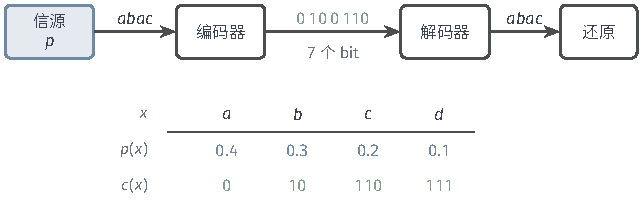
\includegraphics[width=108mm]{figures/07-probability/05-source-coding/tikz/lossless-coding-model/figure.pdf}
 \caption{无损编码的模型。信源（蓝框）按概率表$p$发出消息$abac$，编码器按下方码表把每个符号换成码字并依次拼接（绿色），得到$7$位二进制串；解码器从二进制串精确恢复出同一条消息。}
 \label{fig:lossless-coding-model}
\end{BookInlineFigure}

\paragraph{逐符号与整块，变长与定长}
上面的码表一次处理一个符号，称为逐符号编码。也可以先把$n$个符号组成一块，把整块$x_{1:n}$看成字母表$\mathcal{X}^n$中的一个“大符号”，直接给它分配码字，这就是\term{块编码}（block coding）。整块编码时，被编码的字母表从$\lvert\mathcal{X}\rvert$个元素变成$\lvert\mathcal{X}\rvert^n$个元素，码表的规模随之增长。

码字长度也有两种安排。所有码字等长的称为\term{定长码}（fixed-length code），例如每符号两位的码，或者给每个长度为$n$的块分配同样多位的码；码字长度可以不同的称为\term{变长码}（variable-length code）。定长码不需要寻找码字边界，按固定位数切开即可；变长码要靠码表本身的结构来确定边界。

\paragraph{解码恢复什么}
无损编码要求精确还原，但“还原什么”需要约定。逐符号编码时，解码器要从拼接串$c(x_{1:n})$恢复整条符号序列$x_{1:n}$，而不仅是某一个符号。整块编码时，解码器恢复的是块$x_{1:n}$本身。另一个必须事先约定的是消息长度：解码器是否事先知道$n$，还是要从二进制串本身判断消息在哪里结束。这两种约定的差别在第~\ref{sec:lossless-average-length}节处理确定源时、在第~\ref{sec:lossless-arithmetic}小节处理算术编码的终止时都会出现。

\paragraph{三个评价量}
衡量一个编码方案时，本章分别使用三个量。第一个是按信源概率加权的\term{平均码长}（expected code length），
\begin{equation}
 L(c)=\mathbb{E}[\ell(X)]=\sum_{x\in\mathcal{X}}p(x)\ell(x),
 \label{eq:lossless-average-length}
\end{equation}
它回答长期平均每个符号用多少位：由第~\ref{chap:laws-of-large-numbers}章的大数律，独立编码$n$个符号的总位数除以$n$趋于$L(c)$。第二个是最坏码长$\max_{x}\ell(x)$，它决定缓冲区要准备多大、单条消息最多会多长。第三个是还原错误概率，即解码结果与原消息不同的概率。

三个量回答不同的问题。例中变长码的平均码长是
\[
 L(c)=0.4\times1+0.3\times2+0.2\times3+0.1\times3=1.9 ,
\]
比定长码的$2$少；但最坏码长是$3$，比定长码的$2$多。消息$ddd$用变长码要$9$位，用定长码只要$6$位。所以变长码的“节省”只是平均意义上的，第~\ref{sec:lossless-decodability}节至第~\ref{sec:lossless-methods}节都要求错误概率为零、以平均码长为主要指标，第~\ref{sec:lossless-block-limits}节再允许错误概率为正但趋于零，换取定长的码字。


\section{可解码约束}
\label{sec:lossless-decodability}

码字各不相同，是不是就够了？看下面这张码表：
\[
 a\mapsto0,\qquad b\mapsto010,\qquad c\mapsto01,\qquad d\mapsto10 .
\]
四个码字互不相同，单独收到任何一个码字都能认出是哪个符号。可是收到拼接串$010$时，它既可以是$b$，也可以是$ca$（$01$接$0$），还可以是$ad$（$0$接$10$）。图~\ref{fig:lossless-ambiguous-parse}画出这三种切法。接收方没有分隔符，无法判断发送的是哪一条消息。

\begin{BookInlineFigure}
 \centering
 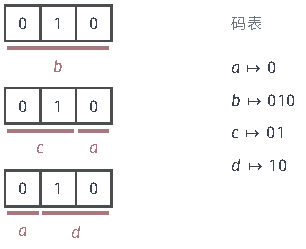
\includegraphics[width=52mm]{figures/07-probability/05-source-coding/tikz/lossless-ambiguous-parse/figure.pdf}
 \caption{码字互不相同、拼接后却有歧义的码。右侧为码表；同一个收到的串$010$（方框）有三种切分方式，红色横线下方是每段对应的符号，分别解读为$b$、$ca$和$ad$。}
 \label{fig:lossless-ambiguous-parse}
\end{BookInlineFigure}

所以要区分两层要求。码$c$称为\term{非奇异码}（nonsingular code），如果不同符号的码字不同，即$c$作为$\mathcal{X}\to\{0,1\}^{*}$的映射是单射。真正需要的是更强的一层：

\begin{definition}[唯一可译码]
\label{def:lossless-uniquely-decodable}
若码$c$的扩展~\eqref{eq:lossless-extension}在所有有限长符号序列上是单射，即对任意$m,n\geq1$与$x_{1:m}\in\mathcal{X}^m$、$y_{1:n}\in\mathcal{X}^n$，
\begin{equation}
 c(x_1)\cdots c(x_m)=c(y_1)\cdots c(y_n)\ \Longrightarrow\ m=n,\ x_{1:m}=y_{1:n},
 \label{eq:lossless-ud}
\end{equation}
则称$c$为\term{唯一可译码}（uniquely decodable code）。
\end{definition}

条件里$m$与$n$可以不同，这是为了把“同一个串能否被切成不同个数的码字”也排除掉。上面的例子中$010$一次切成一个码字、一次切成两个码字，所以那张码表非奇异却不唯一可译。唯一可译码中不能有空码字：若$c(x)$是空串，则$c(x)$与$c(xx)$相同，违反式~\eqref{eq:lossless-ud}。

唯一可译性只说“原则上能切开”，没说怎样切、要往后看多远。下面先看一类可以边读边切的码，再研究所有唯一可译码对码长的共同限制。

\subsection{前缀码}
\label{sec:lossless-prefix-codes}

开头例子的歧义来自一个码字是另一个码字的开头：$0$是$01$和$010$的开头，$01$又是$010$的开头。读到$0$时，解码器不知道这个码字是否已经结束。如果禁止这种情况，读到一个完整码字时就能立刻断开。

\begin{definition}[前缀码]
\label{def:lossless-prefix-code}
若串$s$可写成$s=ut$，则称$u$是$s$的前缀。若码$c$中没有一个码字是另一个码字的前缀，则称$c$为\term{前缀码}（prefix code），也称即时码。
\end{definition}

\paragraph{码树}
二进制串可以画在一棵二叉树上：从根出发，读到$0$走左支，读到$1$走右支，每个串对应一个结点，串长就是结点的深度。码字是树上的一些结点，从根到这些结点的路径合在一起称为\term{码树}（code tree）。“$u$是$s$的前缀”就是“结点$u$在根到结点$s$的路径上”。因此前缀码的码字恰好都是码树的叶结点：没有一个码字结点在另一个码字结点的下方。

图~\ref{fig:lossless-prefix-tree}(a)是贯穿例的码$0,10,110,111$。四个码字都是叶结点，所以它是前缀码。图中(b)是另一张码表$0,01,011,111$，码长同样是$1,2,3,3$，但$a$的码字$0$位于$b$的码字$01$上方，$01$又位于$011$上方，所以它不是前缀码。

\begin{BookInlineFigure}
 \centering
 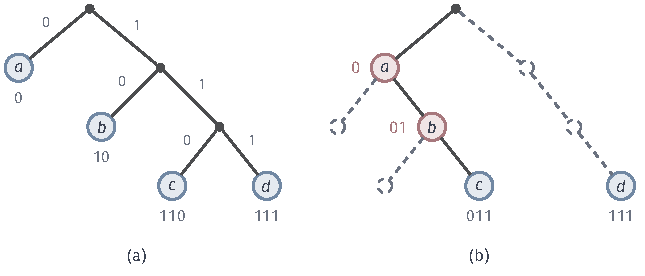
\includegraphics[width=110mm]{figures/07-probability/05-source-coding/tikz/lossless-prefix-tree/figure.pdf}
 \caption{码字作为二叉树的结点，左支读$0$、右支读$1$，结点下方或左侧是它的码字。(a)前缀码$0,10,110,111$，四个码字（蓝圈）都是叶结点。(b)码$0,01,011,111$，码长相同，但$a,b$的码字（红圈）位于其他码字的路径上；虚线和虚圈是路径经过的、不对应码字的结点。}
 \label{fig:lossless-prefix-tree}
\end{BookInlineFigure}

\paragraph{即时解码}
前缀码的解码过程是在码树上行走：从根出发，按收到的位逐步向下，到达叶结点就输出对应符号，然后回到根继续。到达叶结点时，这个码字一定已经结束，因为叶结点下面没有别的码字；而在到达叶结点之前，当前读到的串不是任何码字，也不可能提前断开。

用图~\ref{fig:lossless-prefix-tree}(a)解码$0100110$：读$0$到达叶$a$，输出$a$；读$1,0$到达叶$b$，输出$b$；读$0$输出$a$；读$1,1,0$到达叶$c$，输出$c$。每次输出都在读完该码字最后一位的那一刻完成，不需要看后面的位，这就是“即时”一词的含义。

\begin{theorem}[前缀码唯一可译]
\label{thm:lossless-prefix-ud}
前缀码是唯一可译码。
\end{theorem}

\begin{proof}
设$c(x_1)\cdots c(x_m)=c(y_1)\cdots c(y_n)$，记这个共同的串为$s$。$c(x_1)$与$c(y_1)$都是$s$的前缀，所以较短的一个是较长的一个的前缀。前缀码中这只能在两者相同时发生，于是$c(x_1)=c(y_1)$。前缀码中码字互不相同，所以$x_1=y_1$。

从$s$的两边去掉这个共同的码字，剩下的串仍满足同样的等式，对剩余部分重复上面的论证。每一步去掉同一个码字，直到某一边先用完。若$m<n$，左边用完时剩下的串是空串，右边却还有非空码字$c(y_{m+1})\cdots c(y_n)$；前缀码不含空码字，这不可能，因为空串是任何码字的前缀。所以$m=n$，且各位置的符号都相同。
\end{proof}

\paragraph{唯一可译但不是前缀码}
反过来不成立。图~\ref{fig:lossless-prefix-tree}(b)的码$a\mapsto0$、$b\mapsto01$、$c\mapsto011$、$d\mapsto111$不是前缀码，却是唯一可译码。把每个码字倒过来读，得到$0,10,110,111$，这正是(a)中的前缀码。收到整串后从右向左读，就是在倒序码的码树上即时解码，所以拼接串只有一种切法。

这张码的代价是解码延迟。设收到的串以$0$开头、后面跟着一串$1$。若串在$0111$处结束，它是$ad$；若是$01111$，它是$bd$；若是$011111$，它是$cd$；若是$0111111$，又回到$a$后接两个$d$。第一个码字是$0$、$01$还是$011$，取决于后面$1$的个数除以$3$的余数，解码器必须等这一串$1$全部结束才能确定第一个符号。前缀码没有这种等待，所以实际中几乎总用前缀码；下一小节说明，从码长的角度看，用前缀码也没有任何损失。

\subsection{Kraft–McMillan不等式}
\label{sec:lossless-kraft}

码长越短越好，但不能任意短：$\mathcal{X}$有四个符号，就不可能都用长度$1$的码字，因为长度为$1$的二进制串只有两个。一般地，码长受什么限制？下面先就前缀码回答，再把结论推广到全部唯一可译码。

\paragraph{码字占用的区间}
把码字$s=s_1s_2\cdots s_\ell$看成二进制小数$0.s_1s_2\cdots s_\ell$，它对应$[0,1)$中的区间
\[
 I(s)=\bigl[\,0.s_1\cdots s_\ell,\ 0.s_1\cdots s_\ell+2^{-\ell}\bigr),
\]
即所有以$s$开头的无限二进制展开所组成的数。区间的长度是$2^{-\ell}$：码字越短，占用的区间越长。在码树上，$I(s)$就是结点$s$下面整棵子树的“影子”。

两个码字$u,s$中若$u$是$s$的前缀，则$I(s)\subset I(u)$；若彼此都不是对方的前缀，则两者在某一位上第一次出现不同，一个在那一位取$0$、另一个取$1$，于是$I(u)$与$I(s)$不相交。所以前缀码的码字对应$[0,1)$中两两不交的区间。图~\ref{fig:lossless-kraft-intervals}第一行是贯穿例的码，四个区间恰好铺满$[0,1)$。

\begin{theorem}[Kraft不等式]
\label{thm:lossless-kraft}
设$\mathcal{X}=\{x_1,\dots,x_m\}$，正整数$\ell_1,\dots,\ell_m$。存在码长为$\ell_1,\dots,\ell_m$的二进制前缀码，当且仅当
\begin{equation}
 \sum_{i=1}^{m}2^{-\ell_i}\leq1 .
 \label{eq:lossless-kraft}
\end{equation}
\end{theorem}

\begin{proof}
必要性。前缀码的码字对应$[0,1)$中两两不交的区间，它们的长度之和不超过$[0,1)$的长度$1$，这就是式~\eqref{eq:lossless-kraft}。

充分性。把码长重新编号使$\ell_1\leq\ell_2\leq\cdots\leq\ell_m$，并令
\[
 F_1=0,\qquad F_i=\sum_{j<i}2^{-\ell_j}\quad(i=2,\dots,m).
\]
由式~\eqref{eq:lossless-kraft}，$F_i<1$。每个$2^{-\ell_j}$（$j<i$）都是$2^{-\ell_i}$的整数倍，所以$F_i$也是$2^{-\ell_i}$的整数倍，它的二进制展开在第$\ell_i$位之后全是$0$。取第$i$个码字为$F_i$二进制展开的前$\ell_i$位，于是
\[
 I(c(x_i))=\bigl[F_i,\,F_i+2^{-\ell_i}\bigr)=\bigl[F_i,\,F_{i+1}\bigr) ,
\]
这里$F_{m+1}=\sum_j2^{-\ell_j}\leq1$。这些区间首尾相接、两两不交。若某个码字$u$是另一个码字$s$的前缀，则$I(s)\subset I(u)$，与不交矛盾。所以得到的码是前缀码。
\end{proof}

充分性的证明给出了构造方法：码长从短到长排好，依次在$[0,1)$中从左往右截取长$2^{-\ell_i}$的区间。图~\ref{fig:lossless-kraft-intervals}第二行把这个方法用于码长$2,2,3,4$。依次得到
\[
 F_1=0,\quad F_2=\tfrac14,\quad F_3=\tfrac12,\quad F_4=\tfrac58 ,
\]
码字为$00,01,100,1010$。四个区间只占了$[0,1)$的$11/16$，剩下的$[11/16,1)$没有用上：这组码长满足Kraft不等式但不取等号，说明还有缩短码字的余地，例如把$1010$缩短为$101$仍是前缀码。

\begin{BookInlineFigure}
 \centering
 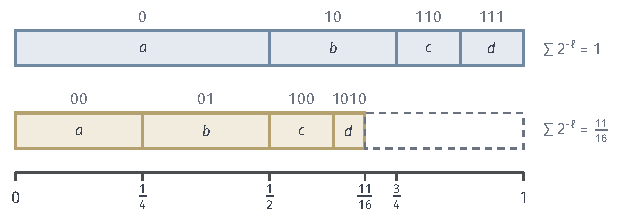
\includegraphics[width=106mm]{figures/07-probability/05-source-coding/tikz/lossless-kraft-intervals/figure.pdf}
 \caption{码字作为$[0,1)$中的二进区间，长度为$\ell$的码字占用长$2^{-\ell}$的区间，区间上方是码字。第一行（蓝）为码$0,10,110,111$，区间铺满$[0,1)$，Kraft和等于$1$。第二行（黄）为码长$2,2,3,4$按充分性证明构造的码$00,01,100,1010$，区间占去$11/16$，虚线框为未用的部分。}
 \label{fig:lossless-kraft-intervals}
\end{BookInlineFigure}

\paragraph{推广到唯一可译码}
唯一可译码的码字可以互为前缀，区间就可能嵌套，上面的必要性证明不再适用。可是码长仍然受同样的限制。McMillan的证明换了一个角度：不看单个码字，而是看把$k$个码字拼起来以后能得到多少种不同的串。

\begin{theorem}[McMillan不等式]
\label{thm:lossless-mcmillan}
任何二进制唯一可译码的码长都满足式~\eqref{eq:lossless-kraft}。
\end{theorem}

\begin{proof}
记$K=\sum_{x\in\mathcal{X}}2^{-\ell(x)}$，$\ell_{\max}=\max_x\ell(x)$。唯一可译码没有空码字，所以每个$\ell(x)\geq1$。固定正整数$k$，把$K$的$k$次方展开：
\[
 K^k=\sum_{x_1\in\mathcal{X}}\cdots\sum_{x_k\in\mathcal{X}}2^{-(\ell(x_1)+\cdots+\ell(x_k))}.
\]
求和的每一项对应一条长度为$k$的符号序列$x_{1:k}$，指数中的和正是它的码串$c(x_{1:k})$的长度。按码串长度$s$分组，记$N_s$为码串长度恰为$s$的序列个数，则
\[
 K^k=\sum_{s=k}^{k\ell_{\max}}N_s\,2^{-s}.
\]
唯一可译性说明不同的序列$x_{1:k}$给出不同的码串，而长度为$s$的二进制串只有$2^s$个，所以$N_s\leq2^s$。代入上式，每一项不超过$1$，项数为$k\ell_{\max}-k+1$，于是
\begin{equation}
 K^k\leq k(\ell_{\max}-1)+1 .
 \label{eq:lossless-mcmillan-count}
\end{equation}
若$K>1$，左边随$k$指数增长，右边只线性增长，$k$足够大时不等式必然被破坏。所以$K\leq1$。
\end{proof}

这个证明的直观是计数。若$K>1$，长序列的数目会比可用的二进制串增长得更快，迟早有两条序列不得不共用同一个码串。图~\ref{fig:lossless-mcmillan-growth}用码长$1,1,2$作例子，此时$K=1.25$。式~\eqref{eq:lossless-mcmillan-count}的右边为$k+1$，从$k=12$起$1.25^{k}$超过它。具体地，$1.25^{12}\approx14.55>13$：长度为$12$的符号序列给出的码串数目，已经超出了相应长度的二进制串所能容纳的数目，这三个码长不可能属于任何唯一可译码。

\begin{BookInlineFigure}
 \centering
 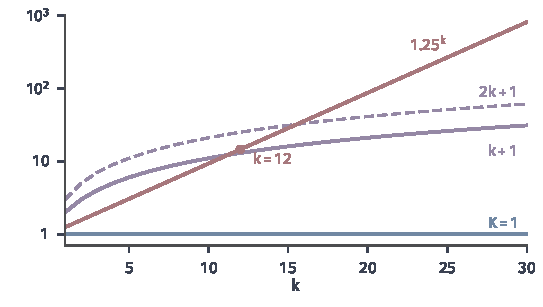
\includegraphics[width=92mm]{figures/07-probability/05-source-coding/matplotlib/lossless-mcmillan-growth/figure.pdf}
 \caption{McMillan计数论证，纵轴为对数坐标。红线为码长$1,1,2$的$K^k=1.25^k$，紫色实线为$\ell_{\max}=2$时的上界$k+1$，二者在红点$k=12$处交叉；紫色虚线为$\ell_{\max}=3$时的上界$2k+1$。蓝线为满足等号的码长$1,2,3,3$，$K^k=1$始终在上界之下。}
 \label{fig:lossless-mcmillan-growth}
\end{BookInlineFigure}

定理~\ref{thm:lossless-kraft}与定理~\ref{thm:lossless-mcmillan}合起来称为\term{Kraft–McMillan不等式}（Kraft–McMillan inequality）：任何唯一可译码的码长满足式~\eqref{eq:lossless-kraft}，而满足式~\eqref{eq:lossless-kraft}的码长都能由前缀码实现。因此，凡是只依赖码长的指标，例如平均码长，在唯一可译码中能达到的值，用前缀码都能达到。前面那张倒序的唯一可译码$0,01,011,111$没有带来任何码长上的好处，只多了解码延迟。

\paragraph{充分性说的是码长}
定理~\ref{thm:lossless-kraft}的充分性只保证“存在”一个具有这些码长的前缀码，并不说任何一种具有这些码长的码字分配都可以唯一解码。码长$1,2,2$满足
\[
 2^{-1}+2^{-2}+2^{-2}=1 ,
\]
按构造得到前缀码$0,10,11$。若随手把码字取成$0,00,11$，码长相同，但$00$既可以是第二个符号，也可以是第一个符号出现两次，不唯一可译。码长合格之后，码字仍要按证明中的方法（或其他保证前缀性的方法）来分配。


\section{平均码长}
\label{sec:lossless-average-length}

Kraft–McMillan不等式说明码长不能都很短：给一个符号分配短码字，就占去了$[0,1)$中一段长区间，留给其他符号的空间随之变小。现在把信源的概率加进来，问：在唯一可译的要求下，平均码长$L(c)$最小能到多少？

\paragraph{熵与自信息}
回答要用到第~\ref{chap:information-measures}章的两个量，这里按本部分的约定以$2$为底重新写出。符号$x$的自信息是$-\log_2p(x)$，单位为bit；信源的熵是自信息的平均，
\begin{equation}
 H(X)=-\sum_{x\in\mathcal{X}}p(x)\log_2p(x).
 \label{eq:lossless-entropy}
\end{equation}
第~\ref{chap:information-measures}章以自然对数计量，单位为nat；以nat计的熵除以$\ln2$，就得到这里以bit计的值。熵是“平均要问几个是非题才能确定结果”：若$p$是均匀分布，$\lvert\mathcal{X}\rvert=2^k$，则恰好需要$k$个是非题，此时$H(X)=k$。

贯穿例的四项自信息为
\[
 \begin{gathered}
 -\log_2 0.4=1.322,\qquad -\log_2 0.3=1.737,\\
 -\log_2 0.2=2.322,\qquad -\log_2 0.1=3.322 ,
 \end{gathered}
\]
按概率加权，
\[
 H(X)=0.4\times1.322+0.3\times1.737+0.2\times2.322+0.1\times3.322=1.846 .
\]

另一个工具是第~\ref{chap:distribution-comparison}章的KL散度。对$\mathcal{X}$上的两个概率质量函数$p$与$r$，若$r(x)>0$对每个$x$成立，
\[
 D_{\mathrm{KL}}(p\Vert r)=\sum_{x\in\mathcal{X}}p(x)\log_2\frac{p(x)}{r(x)}\geq0 ,
\]
等号当且仅当$p=r$。以$2$为底只是把以nat计的值除以$\ln2$，非负性和等号条件不变。

\paragraph{理想码长}
若码长可以取任意正实数，把$\ell(x)$取为$-\log_2p(x)$，Kraft和恰好是
\[
 \sum_x2^{\log_2p(x)}=\sum_xp(x)=1 ,
\]
平均码长恰好是$H(X)$。所以熵是“理想码长”下的平均码长：每个符号的码长等于它的自信息。下面的定理说明，任何唯一可译码都不能比这更短，而整数码长最多比它多出不到一位。

\begin{theorem}[平均码长的熵界]
\label{thm:lossless-entropy-bound}
设信源$X$取值于有限字母表$\mathcal{X}$，$\lvert\mathcal{X}\rvert\geq2$，且$p(x)>0$对每个$x$成立。
\begin{enumerate}
 \item 任何二进制唯一可译码$c$满足
 \begin{equation}
  L(c)\geq H(X),
  \label{eq:lossless-lower-bound}
 \end{equation}
 等号成立当且仅当对每个$x$都有$\ell(x)=-\log_2p(x)$。
 \item 取码长
 \begin{equation}
  \ell(x)=\bigl\lceil-\log_2p(x)\bigr\rceil ,
  \label{eq:lossless-shannon-length}
 \end{equation}
 存在具有这些码长的二进制前缀码，其平均码长满足
 \begin{equation}
  H(X)\leq L(c)<H(X)+1 .
  \label{eq:lossless-upper-bound}
 \end{equation}
\end{enumerate}
\end{theorem}

\begin{proof}
先证第一部分。记$K=\sum_x2^{-\ell(x)}$，由McMillan不等式（定理~\ref{thm:lossless-mcmillan}），$0<K\leq1$。用码长定义一个概率质量函数
\[
 r(x)=\frac{2^{-\ell(x)}}{K},\qquad x\in\mathcal{X},
\]
它的各项为正、和为$1$。由此$\ell(x)=-\log_2r(x)-\log_2K$。代入平均码长与熵之差，
\[
 \begin{aligned}
 L(c)-H(X)&=\sum_xp(x)\ell(x)+\sum_xp(x)\log_2p(x)\\
 &=\sum_xp(x)\log_2\frac{p(x)}{r(x)}-\log_2K .
 \end{aligned}
\]
第一项是$D_{\mathrm{KL}}(p\Vert r)$，非负；$K\leq1$使第二项$-\log_2K\geq0$。所以
\[
 L(c)-H(X)=D_{\mathrm{KL}}(p\Vert r)+\log_2\frac1K\geq0 .
\]
等号要求两项同时为零，即$K=1$且$r=p$，也就是$2^{-\ell(x)}=p(x)$对每个$x$成立。反过来，若$\ell(x)=-\log_2p(x)$，则$L(c)=H(X)$。

再证第二部分。由$\lvert\mathcal{X}\rvert\geq2$且各概率为正，每个$p(x)<1$，所以$-\log_2p(x)>0$，式~\eqref{eq:lossless-shannon-length}给出的$\ell(x)$都是正整数。上取整满足$\ell(x)\geq-\log_2p(x)$，即$2^{-\ell(x)}\leq p(x)$，求和得
\[
 \sum_x2^{-\ell(x)}\leq\sum_xp(x)=1 .
\]
由定理~\ref{thm:lossless-kraft}，存在具有这些码长的前缀码。又因为$\ell(x)<-\log_2p(x)+1$，乘以$p(x)$求和，
\[
 L(c)<\sum_xp(x)\bigl(-\log_2p(x)\bigr)+1=H(X)+1 .
\]
左边的不等号由第一部分得到，因为前缀码是唯一可译码。
\end{proof}

证明把$L(c)-H(X)$拆成两部分，它们分别说明码长损失从哪里来。$D_{\mathrm{KL}}(p\Vert r)$衡量码长所“暗含”的概率$r$与真实概率$p$的差距：码长$\ell(x)$相当于假定$x$的概率是$2^{-\ell(x)}$。$\log_2(1/K)$衡量Kraft不等式没有取等号所浪费的空间，即$[0,1)$中没有被码字占用的部分。

用贯穿例检验这一分解。第~\ref{sec:lossless-model}节的码长$1,2,3,3$满足$K=1$，第二项为零，暗含的概率是
\[
 r=\bigl(\tfrac12,\tfrac14,\tfrac18,\tfrac18\bigr),
\]
冗余$1.9-1.846=0.054$全部来自$D_{\mathrm{KL}}(p\Vert r)=0.054$：它把$a$的概率当成$0.5$、把$d$的概率当成$0.125$，与真实的$0.4$和$0.1$有偏差。下文的Shannon码长$2,2,3,4$给出$K=11/16$，浪费的空间贡献
\[
 \log_2\frac{16}{11}=0.541,
\]
暗含的概率$r=(4,4,2,1)/11$与$p$很接近，KL散度只有$0.013$。两项相加为$0.554$，正是它的冗余$2.4-1.846$。Shannon码的损失几乎全在没有用满的Kraft和上。

按式~\eqref{eq:lossless-shannon-length}取码长并按定理~\ref{thm:lossless-kraft}的方法分配码字，得到的码称为\term{Shannon码}（Shannon code）。平均码长与熵之差$L(c)-H(X)$称为码的\term{冗余}（redundancy）。

\paragraph{贯穿例}
贯穿例中$p(x)$都小于$1$，定理适用。Shannon码长为
\[
 \lceil1.322\rceil=2,\quad\lceil1.737\rceil=2,\quad\lceil2.322\rceil=3,\quad\lceil3.322\rceil=4 ,
\]
Kraft和为$11/16$，码字由图~\ref{fig:lossless-kraft-intervals}第二行给出。平均码长为
\[
 L=0.4\times2+0.3\times2+0.2\times3+0.1\times4=2.4 ,
\]
确实落在$[1.846,\,2.846)$中。可是它比两位定长码还长。第~\ref{sec:lossless-model}节的码$0,10,110,111$平均只要$1.9$位，冗余为$0.054$。式~\eqref{eq:lossless-upper-bound}只保证冗余小于$1$，并不说明Shannon码是好的码；平均码长最短的码由第~\ref{sec:lossless-huffman}小节构造。

\paragraph{冗余是平均量}
冗余小于$1$说的是平均。逐个符号看，码长与自信息之差$\ell(x)+\log_2p(x)$各不相同，图~\ref{fig:lossless-length-vs-selfinfo}把它们画在一起。对Shannon码，这个差在$[0,1)$中，四个符号分别是
\[
 0.678,\quad 0.263,\quad 0.678,\quad 0.678 .
\]
对码$0,10,110,111$，四个差分别是
\[
 -0.322,\quad 0.263,\quad 0.678,\quad -0.322 ,
\]
其中$a$与$d$的码长比自信息还短。所以“整数码长带来不到一位的冗余”不是说每条消息都比它的自信息长同样多：个别符号可以比自信息短，个别可以长将近一位，下界$L\geq H$只约束加权平均。

\begin{BookInlineFigure}
 \centering
 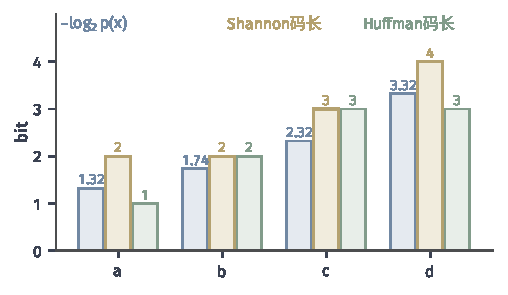
\includegraphics[width=86mm]{figures/07-probability/05-source-coding/matplotlib/lossless-length-vs-selfinfo/figure.pdf}
 \caption{贯穿例中每个符号的自信息$-\log_2p(x)$（蓝）、Shannon码长$\lceil-\log_2p(x)\rceil$（黄）和第~\ref{sec:lossless-model}节码表的码长（绿）。Shannon码长总不小于自信息；后一张码表中$a$与$d$的码长小于自信息，平均码长$1.9$却仍不小于熵$1.846$。}
 \label{fig:lossless-length-vs-selfinfo}
\end{BookInlineFigure}

\paragraph{冗余可以接近一位}
上界中的$+1$不能改进成更小的常数。取二元信源$\mathcal{X}=\{0,1\}$，$p(1)=\theta$。任何唯一可译码的码字至少一位，所以平均码长至少为$1$；而熵
\[
 H(\theta)=-\theta\log_2\theta-(1-\theta)\log_2(1-\theta)
\]
在$\theta\to0$时趋于$0$。$\theta=0.1$时$H=0.469$，最优码仍要$1$位，冗余$0.531$；$\theta$越小，冗余越接近$1$。图~\ref{fig:lossless-binary-bounds}画出这一情形。问题在于每个符号至少要花一位：概率极不均匀时，一个符号所含的信息远少于一位，逐符号编码无法用“半位”来记录它。第~\ref{sec:lossless-block-limits}节把多个符号合成一块编码，正是为了把这一位摊到许多符号上。

\begin{BookInlineFigure}
 \centering
 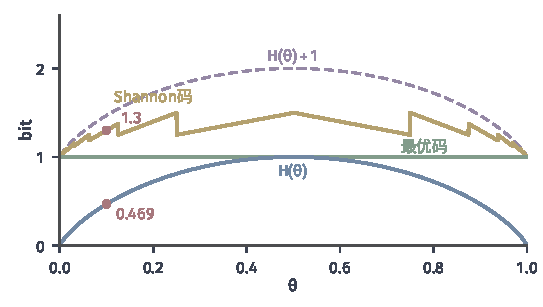
\includegraphics[width=92mm]{figures/07-probability/05-source-coding/matplotlib/lossless-binary-bounds/figure.pdf}
 \caption{二元信源$p(1)=\theta$的逐符号编码。蓝线为熵$H(\theta)$，紫色虚线为上界$H(\theta)+1$，黄线为Shannon码的平均码长，绿线为最优码的平均码长$1$。红点标出$\theta=0.1$处的$H=0.469$与Shannon码长$1.3$。黄线在$\theta=1/2$处另有一个孤立的取值$1$，图中未画出。}
 \label{fig:lossless-binary-bounds}
\end{BookInlineFigure}

\paragraph{确定源}
定理~\ref{thm:lossless-entropy-bound}要求至少两个符号有正概率。若只有一个符号$x_0$，$p(x_0)=1$，则$H(X)=0$，式~\eqref{eq:lossless-shannon-length}给出的码长是$0$，即空码字。这时要看解码器知道什么。

若消息长度$n$事先约定，接收方知道消息必定是$x_0x_0\cdots x_0$（$n$个），什么都不必发送，平均码长为$0$，等于熵。若长度没有约定，空码字无法告诉接收方发出了几个符号：$n=1$和$n=5$的消息都编成空串。由第~\ref{sec:lossless-decodability}节，唯一可译码不含空码字，每个符号至少一位，平均码长至少为$1$；另一种做法是单独传送长度$n$，所需位数随$n$增长，但这已不是逐符号编码的问题。所以确定源的“零码长”只在长度已知时成立，这正是定理把它排除在外的原因。


\section{编码方法}
\label{sec:lossless-methods}

前两节确定了标准：解码必须唯一，评价看平均码长，下界是熵。Shannon码满足上界，却可能比简单的码还差。本节构造两种实际使用的编码。Huffman编码针对给定的有限符号表，直接求出平均码长最短的前缀码；算术编码不给单个符号分配码字，而是把整条消息对应到$[0,1)$中的一个小区间。两者处理的对象不同，比较时要统一被编码的对象和消息的终止规则。

\subsection{Huffman编码}
\label{sec:lossless-huffman}

在所有二进制前缀码中，哪一个的平均码长最小？前缀码只有有限多种“有用的”码长组合，原则上可以穷举，但符号多时组合数巨大。\term{Huffman编码}（Huffman coding）给出一个只需反复合并的构造\scite{vision-huffman1952}。

\paragraph{主要思想}
从码树的角度看，平均码长是各叶结点深度按概率加权的和。概率小的符号应当放在深处，而最深处的两片叶子一定是兄弟。把这两片叶子合并成它们的父结点，问题就变成一个少一个符号的同类问题。Huffman编码的做法是：每次把概率最小的两个符号合并成一个新符号，新符号的概率是两者之和，直到只剩一个符号；再沿合并的过程从根往下分配$0$和$1$。

要说明这样做是最优的，需要两步：先证明存在一个最优码，其中概率最小的两个符号恰好是最深处的一对兄弟；再证明合并之后的问题与原问题的最优值只相差一个常数。

称前缀码$c^{\star}$为最优的，如果它的平均码长在所有前缀码中最小。最优码存在：任取一个前缀码$c_0$，平均码长不超过$L(c_0)$的前缀码满足
\[
 \ell(x)\leq\frac{L(c_0)}{\min_y p(y)}\quad\text{对每个}x ,
\]
只有有限多种码长组合，其中必有平均码长最小的一个。

\begin{lemma}[最优码的结构]
\label{lem:lossless-optimal-structure}
设$\lvert\mathcal{X}\rvert\geq2$，各$p(x)>0$，$u,v$是概率最小的两个符号（有并列时任取）。则存在最优前缀码$c^{\star}$，使得：
\begin{enumerate}
 \item 若$p(x)>p(y)$，则$\ell(x)\leq\ell(y)$；
 \item $c^{\star}(u)$与$c^{\star}(v)$长度相同且为最大码长，两者只有最后一位不同。
\end{enumerate}
\end{lemma}

\begin{proof}
第一条对每个最优码都成立。若$p(x)>p(y)$而$\ell(x)>\ell(y)$，交换$x,y$的码字，得到的仍是前缀码，平均码长的变化为
\[
 \begin{aligned}
 &p(x)\ell(y)+p(y)\ell(x)-p(x)\ell(x)-p(y)\ell(y)\\
 &\qquad=-\bigl(p(x)-p(y)\bigr)\bigl(\ell(x)-\ell(y)\bigr)<0 ,
 \end{aligned}
\]
与最优性矛盾。

其次，在任一最优码中，设$s$是一个最长的码字，把$s$的最后一位取反得到串$s'$，称为$s$的兄弟。$s'$一定是码字。否则，任何以$s'$开头的码字长度都不小于$\lvert s\rvert$，而$s$已是最长，于是没有码字以$s'$开头；这时删去$s$的最后一位，得到的码仍是前缀码，平均码长减少$p(\cdot)>0$，矛盾。所以最长码字成对出现，每对是兄弟。

最后，取一对最长的兄弟码字，设它们属于符号$y,y'$。把$u$与$y$的码字交换，再把$v$与$y'$的码字交换（若$u$或$v$本来就是$y$或$y'$，相应的交换省去）。由于$p(u)\leq p(y)$而$\ell(u)\leq\ell(y)$（$y$的码长是最大码长），按上面的计算，这一交换使平均码长的变化为
\[
 \bigl(p(y)-p(u)\bigr)\bigl(\ell(u)-\ell(y)\bigr)\leq0 ,
\]
第二次交换同理。交换后的码平均码长不增，仍是最优码，且$u,v$占据最深的一对兄弟。第一条对它仍成立。
\end{proof}

图~\ref{fig:lossless-huffman-exchange}用贯穿例演示交换。码树的深度固定为$1,2,3,3$，若把概率最大的$a$放在深度$3$、概率最小的$d$放在深度$1$，平均码长为$2.5$；交换两者后，平均码长减少
\[
 (0.4-0.1)\times(3-1)=0.6 ,
\]
变为$1.9$。

\begin{BookInlineFigure}
 \centering
 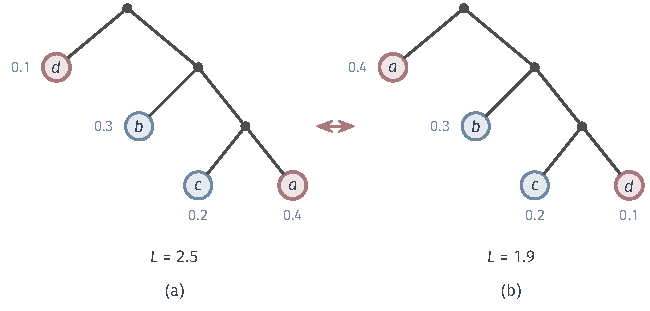
\includegraphics[width=110mm]{figures/07-probability/05-source-coding/tikz/lossless-huffman-exchange/figure.pdf}
 \caption{交换论证。两棵码树形状相同，叶结点旁为概率。(a)把概率$0.4$的$a$放在深度$3$、概率$0.1$的$d$放在深度$1$，平均码长$2.5$。(b)交换两片红色叶子后平均码长降为$1.9$。}
 \label{fig:lossless-huffman-exchange}
\end{BookInlineFigure}

接下来比较合并前后的问题。设$u,v$如引理所述，构造缩减的字母表$\mathcal{X}'$：去掉$u,v$，加入一个新符号$z$，其概率为$p'(z)=p(u)+p(v)$，其余符号概率不变。给定$\mathcal{X}'$上的前缀码$c'$，令
\[
 c(u)=c'(z)0,\qquad c(v)=c'(z)1,\qquad c(x)=c'(x)\ (x\neq u,v),
\]
即把叶子$z$展开成两片兄弟叶子。$c$仍是前缀码，平均码长满足
\begin{equation}
 L(c)=L(c')+p(u)+p(v) ,
 \label{eq:lossless-huffman-reduction}
\end{equation}
因为只有$u,v$的码长比$z$多一位。反过来，若$\mathcal{X}$上的前缀码中$u,v$是兄弟叶子，把它们合并成父结点就得到$\mathcal{X}'$上的前缀码，平均码长的关系同样是式~\eqref{eq:lossless-huffman-reduction}。

\begin{theorem}[Huffman编码的最优性]
\label{thm:lossless-huffman-optimal}
设$\mathcal{X}$有限，$\lvert\mathcal{X}\rvert\geq2$，各$p(x)>0$。Huffman编码的平均码长在所有二进制唯一可译码中最小。
\end{theorem}

\begin{proof}
由Kraft–McMillan不等式，唯一可译码能实现的码长都能由前缀码实现，所以只需与前缀码比较。对符号个数$m=\lvert\mathcal{X}\rvert$作归纳。$m=2$时Huffman编码给出码字$0,1$，平均码长为$1$；唯一可译码不含空码字，平均码长至少为$1$，结论成立。

设结论对$m-1$个符号成立。Huffman编码先合并概率最小的$u,v$，在缩减字母表$\mathcal{X}'$上得到Huffman码$h'$，再把$z$展开，得到$\mathcal{X}$上的码$h$。由式~\eqref{eq:lossless-huffman-reduction}，
\[
 L(h)=L(h')+p(u)+p(v).
\]
取引理~\ref{lem:lossless-optimal-structure}给出的最优码$c^{\star}$，其中$u,v$是兄弟叶子，合并得到$\mathcal{X}'$上的前缀码$c'$，同样有
\[
 L(c^{\star})=L(c')+p(u)+p(v).
\]
由归纳假设，$h'$在$\mathcal{X}'$上最优，$L(h')\leq L(c')$。两式相减得$L(h)\leq L(c^{\star})$，所以$h$也是最优码。
\end{proof}

式~\eqref{eq:lossless-huffman-reduction}还给出一个算平均码长的捷径：每合并一次，平均码长增加被合并两项的概率之和。所以Huffman码的平均码长等于各次合并所得新结点的概率之和。

\paragraph{计算过程}
下面在贯穿例$p=(0.4,0.3,0.2,0.1)$上逐步执行。

\needspace{6\baselineskip}
\paragraph{变量}
\begin{itemize}
 \item 待合并结点的集合$\mathcal{Q}$：每个结点是一棵子树，带有权重，即子树中所有叶结点的概率之和。实现时用按权重排序的优先队列。
 \item 子树内部的连接：每个内部结点记住它的两个子结点，以及分别通向它们的边上的位$0$或$1$。
 \item 并列规则：权重相同时，先进入$\mathcal{Q}$的结点先取出。原始符号在初始化时进入，合并产生的结点后进入。
\end{itemize}

\paragraph{初始化}
每个符号是一个只有一片叶子的子树，权重为它的概率，全部放入$\mathcal{Q}$。例中
\[
 \mathcal{Q}=\{a:0.4,\ b:0.3,\ c:0.2,\ d:0.1\}.
\]

\needspace{6\baselineskip}
\paragraph{每轮更新}
当$\mathcal{Q}$中多于一个结点时：
\begin{enumerate}
 \item \textbf{取出两个最小权重。}从$\mathcal{Q}$中依次取出权重最小的结点$s_1$与次小的结点$s_2$。例中第一轮取出$d$（$0.1$）与$c$（$0.2$）。
 \item \textbf{合并。}新建内部结点$t$，以$s_1,s_2$为子结点，通向$s_1$的边记$0$，通向$s_2$的边记$1$，权重为两者之和。例中第一轮
 \[
  t_1=\{d,c\},\qquad 0.1+0.2=0.3 .
 \]
 \item \textbf{放回。}把$t$放入$\mathcal{Q}$。例中第一轮后
 \[
  \mathcal{Q}=\{a:0.4,\ b:0.3,\ t_1:0.3\}.
 \]
\end{enumerate}
例中第二轮，$b$与$t_1$的权重都是$0.3$，按并列规则先取出$b$，再取出$t_1$，合并为权重$0.6$的结点$t_2$，$b$一侧记$0$，$t_1$一侧记$1$：
\[
 \mathcal{Q}=\{a:0.4,\ t_2:0.6\}.
\]
第三轮取出$a$与$t_2$，合并为权重$1$的根结点$t_3$，$a$一侧记$0$，$t_2$一侧记$1$，$\mathcal{Q}$中只剩一个结点，合并结束。图~\ref{fig:lossless-huffman-steps}画出各轮之后的森林。

\begin{BookInlineFigure}
 \centering
 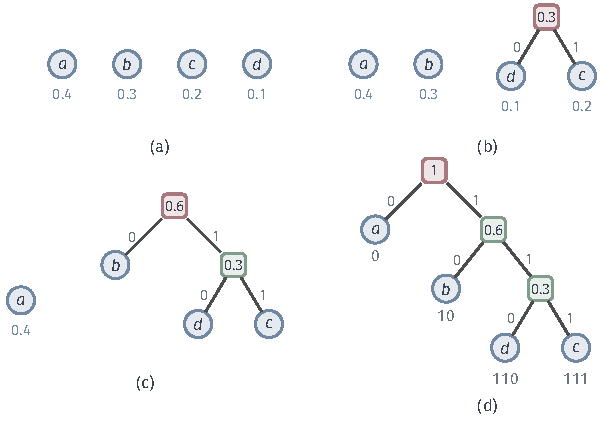
\includegraphics[width=102mm]{figures/07-probability/05-source-coding/tikz/lossless-huffman-steps/figure.pdf}
 \caption{贯穿例的Huffman合并。蓝圈为原始符号及其概率，方框为合并产生的结点及其权重，红框是该轮新产生的结点，边旁为分配的位。(a)初始；(b)合并$d,c$；(c)合并$b$与$\{d,c\}$；(d)合并$a$得到根，叶结点下方为码字。}
 \label{fig:lossless-huffman-steps}
\end{BookInlineFigure}

\paragraph{读出码字}
从根出发走到每片叶子，依次写下经过的位，就是该符号的码字。例中
\[
 a\mapsto0,\qquad b\mapsto10,\qquad d\mapsto110,\qquad c\mapsto111 .
\]
码长为$1,2,3,3$。按合并新结点的权重求和，
\[
 L=0.3+0.6+1.0=1.9 ,
\]
与按定义逐项计算一致。最终得到的码长与第~\ref{sec:lossless-model}节的码表相同，只是$c,d$的码字互换；两者长度相同，平均码长都是$1.9$，冗余为$1.9-1.846=0.054$。由定理~\ref{thm:lossless-huffman-optimal}，在这个概率表下没有平均码长小于$1.9$的唯一可译码。

\paragraph{算法分析}
用二叉堆实现优先队列时，每轮取出两次、放入一次，各需$O(\log m)$次比较，共$m-1$轮，总计算量为$O(m\log m)$；若概率已经排好序，可以用两个先进先出队列在$O(m)$时间内完成。并列规则不同时，得到的码树和码长都可能不同，但由定理~\ref{thm:lossless-huffman-optimal}，平均码长相同。最长码字可以长达$m-1$位，例如概率按$1/2,1/4,1/8,\dots$递减时码树退化成一条链。

最优性的范围要说清楚。定理只断言：对一个给定的有限字母表和给定的概率表，在逐符号的二进制唯一可译码中，Huffman码平均码长最短。它不说明每个符号至少要花这么多位；若把若干符号合成一块再编码，被编码的字母表就换成了$\mathcal{X}^n$，有$\lvert\mathcal{X}\rvert^n$个“符号”，Huffman码要对这个大字母表重新构造，平均到每个原始符号上可以更短（第~\ref{sec:lossless-block-limits}节）。代价是码表规模随块长指数增长。

\subsection{算术编码}
\label{sec:lossless-arithmetic}

Huffman码给每个符号整数位，概率极不均匀时，一个符号可能只含零点几位信息，却至少要花一位。另一条路是不给符号分配码字，而给整条消息分配码字。\term{算术编码}（arithmetic coding）用一个逐步缩小的区间来做这件事\scite{math-witten1987arithmetic}。

\paragraph{主要思想}
把$[0,1)$看成单位质量，按概率分给各个符号：贯穿例中$a$占$[0,0.4)$，$b$占$[0.4,0.7)$，$c$占$[0.7,0.9)$，$d$占$[0.9,1)$。读到第一个符号，就留下它的那一段；在这一段里再按同样的比例分给四个符号，读到第二个符号再留下相应的一小段；如此继续。读完整条消息时剩下的区间，长度恰好是这条消息的概率。

用公式写出来。给$\mathcal{X}$中的符号排定顺序，记累积概率
\[
 F(x)=\sum_{y\prec x}p(y),
\]
其中$y\prec x$表示$y$排在$x$之前。贯穿例按$a,b,c,d$排序，$F(a)=0$，$F(b)=0.4$，$F(c)=0.7$，$F(d)=0.9$。消息$x_{1:n}$对应的区间$[\mathrm{lo}_k,\mathrm{lo}_k+w_k)$按下式逐步更新：
\begin{equation}
 \mathrm{lo}_0=0,\quad w_0=1;\qquad
 \mathrm{lo}_k=\mathrm{lo}_{k-1}+w_{k-1}F(x_k),\quad w_k=w_{k-1}\,p(x_k).
 \label{eq:lossless-arith-update}
\end{equation}
第$k$步把当前区间按比例切开，留下第$k$个符号的那一份。由此$w_n=\prod_{k}p(x_k)$，按式~\eqref{eq:lossless-product}正是$p(x_{1:n})$。记$J(x_{1:n})=[\mathrm{lo}_n,\mathrm{lo}_n+w_n)$。

固定消息长度$n$，所有长度为$n$的消息的区间$J(x_{1:n})$两两不交，并且铺满$[0,1)$。对$n$归纳：$n=0$时只有$[0,1)$；长度为$k$的消息的区间由长度为$k-1$的前缀的区间按概率切成$\lvert\mathcal{X}\rvert$份得到，各份不交且铺满原区间。

剩下的问题是怎样用尽量少的位说出“消息的区间是哪一个”。办法与Kraft不等式的证明相同：找一个完全落在$J(x_{1:n})$内的二进区间，发送它对应的二进制串。取
\begin{equation}
 \ell=\Bigl\lceil\log_2\frac{1}{w_n}\Bigr\rceil+1,\qquad
 k=\bigl\lceil\mathrm{lo}_n2^{\ell}\bigr\rceil ,
 \label{eq:lossless-arith-codeword}
\end{equation}
码字是整数$k$的$\ell$位二进制表示（不足$\ell$位时前面补$0$），它对应二进区间$[k2^{-\ell},(k+1)2^{-\ell})$。

这个二进区间落在$J(x_{1:n})$内。左端：$k\geq\mathrm{lo}_n2^{\ell}$，所以$k2^{-\ell}\geq\mathrm{lo}_n$。右端：$k<\mathrm{lo}_n2^{\ell}+1$，再由$\ell$的取法$2^{-\ell}\leq w_n/2$，于是
\[
 (k+1)2^{-\ell}<\mathrm{lo}_n+2\cdot2^{-\ell}\leq\mathrm{lo}_n+w_n .
\]
同一长度的不同消息区间不交，它们的二进区间也不交，所以这些码字中没有一个是另一个的前缀：对固定的$n$，算术编码是$\mathcal{X}^n$上的前缀码。码长满足
\begin{equation}
 \ell<\log_2\frac{1}{p(x_{1:n})}+2 ,
 \label{eq:lossless-arith-length}
\end{equation}
对消息取期望，平均码长小于$nH(X)+2$，每符号小于$H(X)+2/n$。消息越长，这额外的两位摊得越薄。

解码是同一过程的逆向。设收到码字，算出$v=k2^{-\ell}$，它落在$J(x_{1:n})$中。第一个符号是唯一满足$F(x)\leq v<F(x)+p(x)$的$x$；把$v$换成$(v-F(x_1))/p(x_1)$，即在留下的子区间中重新标定到$[0,1)$，再按同样的规则读出第二个符号，如此重复$n$次。解码器必须使用与编码器完全相同的符号顺序和概率。

\paragraph{计算过程}
下面用贯穿例对消息$abac$逐步演示，$n=4$事先约定。

\needspace{6\baselineskip}
\paragraph{变量}
\begin{itemize}
 \item 概率表$p(x)$与累积概率表$F(x)$：各$\lvert\mathcal{X}\rvert$个数，编码器与解码器共享。
 \item $\mathrm{lo}$：当前区间的左端点。
 \item $w$：当前区间的长度。
 \item 消息长度$n$：事先约定，或按下文的终止规则处理。
\end{itemize}

\paragraph{初始化}
$\mathrm{lo}=0$，$w=1$。例中$F=(0,0.4,0.7,0.9)$，$p=(0.4,0.3,0.2,0.1)$。

\needspace{6\baselineskip}
\paragraph{每轮更新}
对$k=1,\dots,n$，读入符号$x_k$：
\begin{enumerate}
 \item \textbf{移左端。}按式~\eqref{eq:lossless-arith-update}，$\mathrm{lo}\leftarrow\mathrm{lo}+w\,F(x_k)$。
 \item \textbf{缩长度。}$w\leftarrow w\,p(x_k)$。
\end{enumerate}
例中四轮的结果如下（先算左端，再用旧的$w$乘概率）：
\[
 \begin{aligned}
 &a:&\mathrm{lo}&=0+1\times0=0, & w&=1\times0.4=0.4,\\
 &b:&\mathrm{lo}&=0+0.4\times0.4=0.16, & w&=0.4\times0.3=0.12,\\
 &a:&\mathrm{lo}&=0.16+0.12\times0=0.16, & w&=0.12\times0.4=0.048,\\
 &c:&\mathrm{lo}&=0.16+0.048\times0.7=0.1936, & w&=0.048\times0.2=0.0096.
 \end{aligned}
\]
读完$n$个符号后结束，最终区间为
\[
 J(abac)=[0.1936,\,0.2032),\qquad w_4=0.0096=p(abac).
\]

\paragraph{输出码字}
由式~\eqref{eq:lossless-arith-codeword}，
\[
 \ell=\lceil6.703\rceil+1=8,\qquad k=\lceil0.1936\times256\rceil=\lceil49.56\rceil=50 ,
\]
码字是$50$的$8$位二进制表示$00110010$，对应二进区间
\[
 [50/256,\,51/256)=[0.1953,\,0.1992)\subset[0.1936,\,0.2032).
\]
图~\ref{fig:lossless-arith-intervals}逐行画出区间的缩小过程。这条消息的自信息是$\log_2(1/0.0096)=6.703$位，算术编码用了$8$位，比上一小节的Huffman码字串$0\,10\,0\,111$多一位。对这样短的消息，式~\eqref{eq:lossless-arith-length}中的两位额外开销相当可观；它的好处要在长消息中才显现。

\begin{BookInlineFigure}
 \centering
 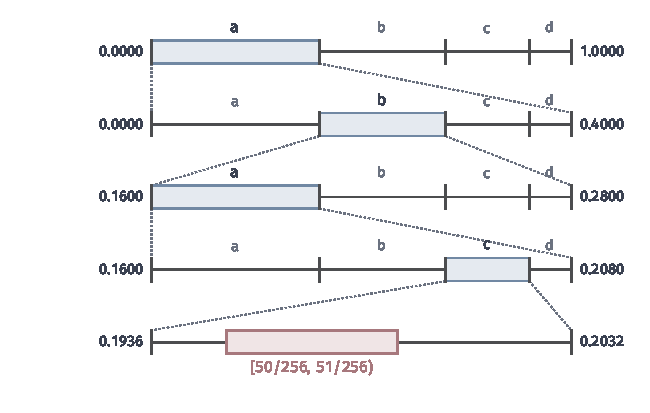
\includegraphics[width=110mm]{figures/07-probability/05-source-coding/matplotlib/lossless-arith-intervals/figure.pdf}
 \caption{算术编码消息$abac$。每一行把当前区间放大到同样宽度，两侧数字为区间端点，按$4:3:2:1$切给$a,b,c,d$；浅蓝格是读到的符号留下的子区间，虚线把它放大到下一行。最后一行是最终区间$[0.1936,0.2032)$，红框是码字$00110010$对应的二进区间。}
 \label{fig:lossless-arith-intervals}
\end{BookInlineFigure}

同样长度的另一条消息$abad$只在最后一步不同：$\mathrm{lo}=0.16+0.048\times0.9=0.2032$，$w=0.0048$，于是$\ell=\lceil7.703\rceil+1=9$，$k=\lceil0.2032\times512\rceil=105$，码字为$001101001$。它与$00110010$在第$6$位就不同，谁也不是谁的前缀，这正是两条消息的区间$[0.1936,0.2032)$与$[0.2032,0.2080)$不交的结果。

\paragraph{解码}
解码器收到$00110010$，得$v=50/256=0.1953$，逐步读出：
\[
 \begin{aligned}
 &v=0.1953\in[0,0.4) &&\Rightarrow a, & v&\leftarrow0.1953/0.4=0.4883,\\
 &v=0.4883\in[0.4,0.7) &&\Rightarrow b, & v&\leftarrow(0.4883-0.4)/0.3=0.2943,\\
 &v=0.2943\in[0,0.4) &&\Rightarrow a, & v&\leftarrow0.2943/0.4=0.7357,\\
 &v=0.7357\in[0.7,0.9) &&\Rightarrow c .
 \end{aligned}
\]
读满$n=4$个符号后停止，恢复出$abac$。

\paragraph{终止规则}
上面的码对固定的$n$是前缀码，不同长度的消息之间却可能冲突：同一个码字所在的二进区间，既落在某条长度为$4$的消息的区间里，也落在它的前缀$aba$的区间里。所以接收方必须知道消息在哪里结束。常用两种约定。一是事先约定或单独传送长度$n$；单独传送时，用一个整数的前缀码，大约需要$2\log_2n$位。二是在字母表中加入终止符号，给它一个小概率$\varepsilon$，其余符号的概率乘以$1-\varepsilon$；消息总以终止符号结束，于是“消息加终止符”组成的集合中没有一条是另一条的前缀。终止符号的代价是消息末尾多出$\log_2(1/\varepsilon)$位，每个普通符号多出$\log_2(1/(1-\varepsilon))$位。

\paragraph{有限精度}
上面的计算用的是精确实数，消息长时$w$小到无法用浮点数表示。实际实现用整数：概率表写成整数频数$f(x)$，总和为$T$；区间端点用$B$位整数表示。每读一个符号，按频数比例切分整数区间并向下取整。每当区间整个落在$[0,1/2)$或$[1/2,1)$中，最高位已经确定，立即输出这一位，并把区间放大一倍，使区间长度保持在一个固定范围内；区间跨越中点但很窄时，记下“待定位”的个数，等以后确定方向再一并输出。

整数实现能正确解码的关键，是编码器与解码器做完全相同的整数运算和取整：只要两边一致，取整只是把每个子区间的长度稍微改动，改动后的子区间仍两两不交、铺满当前区间。取整的代价是码长比式~\eqref{eq:lossless-arith-length}稍长，$B$足够大时这个损失很小。此外每个可能出现的符号都需要$f(x)\geq1$，否则它的子区间长度为零，无法编码。

\paragraph{模型与实际概率}
编码器和解码器用的概率表$q$称为模型，它可以与信源的真实分布$p$不同。只要两边用同一个$q$，并且消息中出现的每个符号都有$q(x)>0$，上面的论证不变，只需把$p$换成$q$：码长满足
\[
 \ell<\log_2\frac{1}{q(x_{1:n})}+2 ,
\]
解码仍然正确。模型不准只让码长变长，对独立同分布消息，平均每符号码长约为$H(X)+D_{\mathrm{KL}}(p\Vert q)$，第~\ref{sec:lossless-finite-resources}节将给出这一点的精确界。

若模型给一个实际出现的符号零概率，$q(x_k)=0$，则$w$在这一步变成$0$，区间消失，这条消息无法编码。这不是“码长变长”的问题，而是编码本身无法继续。所以模型必须给每个可能出现的符号留下正概率。

模型也可以随已读的符号改变，只要编码器和解码器按同一规则更新：把式~\eqref{eq:lossless-arith-update}中的$p(x_k)$与$F(x_k)$换成依赖于$x_{1:k-1}$的条件概率与累积概率，区间长度就变成这些条件概率的乘积，上面的论证照样成立。这使算术编码可以配合任意按顺序给出概率的模型，而Huffman码要求事先给定一个固定的概率表。

\paragraph{与Huffman编码比较}
比较两种方法时，必须让它们编码同一个对象，按同一个终止规则。Huffman码是逐符号的前缀码，消息结束靠约定长度或额外的码字；按长度为$n$的整条消息计算，它的平均码长为$n\times1.9$，每符号$1.9$位。算术编码在$n$已知时，每符号平均码长小于
\[
 H(X)+\frac{2}{n}=1.846+\frac{2}{n} ,
\]
$n=4$时这个上界是$2.346$，比Huffman码差；$n=40$时为$1.896$，已低于Huffman码。

图~\ref{fig:lossless-arith-length}在一条长$400$的随机消息上验证这些数值。用真实模型$p$编码时，每符号码长从短消息时的约$3$位逐步降到$1.855$位，接近熵$1.846$；用均匀模型$q(x)=1/4$编码时，码长恰为$2n+1$，每符号趋于$2$，即$H+D_{\mathrm{KL}}(p\Vert q)=1.846+0.154$。右图显示，在每个前缀长度上，码长与自信息之差都落在$[1,2)$中，这正是式~\eqref{eq:lossless-arith-codeword}的取整与$+1$造成的。

\begin{BookInlineFigure}
 \centering
 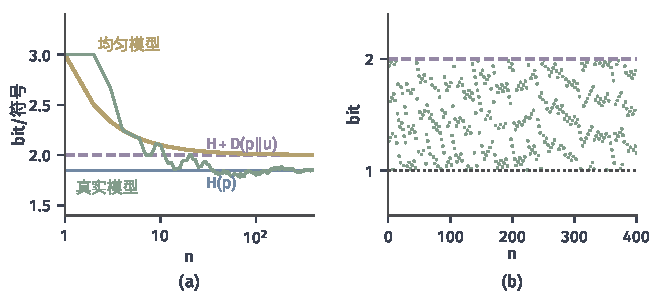
\includegraphics[width=110mm]{figures/07-probability/05-source-coding/matplotlib/lossless-arith-length/figure.pdf}
 \caption{一条由贯穿例信源独立生成、长$400$的消息（随机种子$7$）。(a)各前缀长度$n$下算术编码的每符号码长，横轴为对数坐标：绿线用真实模型，黄线用均匀模型；蓝线为熵$H=1.846$，紫色虚线为$H+D_{\mathrm{KL}}(p\Vert u)=2$。(b)真实模型下码长与消息自信息之差，所有点落在$[1,2)$中。}
 \label{fig:lossless-arith-length}
\end{BookInlineFigure}


\section{块编码的压缩极限}
\label{sec:lossless-block-limits}

逐符号编码的冗余可以接近一位，原因是每个符号至少花一位。把$n$个符号合成一块编码，可以从两个方向利用这一点。一是仍要求每块精确还原，但让整数码长的取整损失摊到$n$个符号上；二是放弃对极少数块的还原，只给高概率的块编号，从而使用固定长度的码字。两条路都把每符号所需的位数压到熵$H(X)$，但允许的码长形式和错误要求不同。本节设$X_1,X_2,\dots$独立同分布，服从字母表$\mathcal{X}$上的$p$。

\subsection{零错误的变长块编码}
\label{sec:lossless-variable-block}

把块$x_{1:n}$看作字母表$\mathcal{X}^n$中的一个符号，它的概率由式~\eqref{eq:lossless-product}给出。对这个大字母表直接应用定理~\ref{thm:lossless-entropy-bound}，需要知道块的熵。

\begin{lemma}[独立块的熵]
\label{lem:lossless-block-entropy}
若$X_1,\dots,X_n$独立同分布，则
\begin{equation}
 H(X_{1:n})=nH(X_1).
 \label{eq:lossless-block-entropy}
\end{equation}
\end{lemma}

\begin{proof}
由式~\eqref{eq:lossless-product}，块的自信息是各符号自信息之和：
\[
 -\log_2p(x_{1:n})=\sum_{i=1}^{n}\bigl(-\log_2p(x_i)\bigr).
\]
在$x_{1:n}$处取值为$X_{1:n}$，两边取期望，由期望的线性性与同分布，
\[
 \begin{aligned}
 H(X_{1:n})&=\mathbb{E}\Bigl[\sum_{i=1}^{n}-\log_2p(X_i)\Bigr]\\
 &=\sum_{i=1}^{n}H(X_i)=nH(X_1). \qedhere
 \end{aligned}
\]
\end{proof}

\begin{theorem}[变长块编码]
\label{thm:lossless-variable-block}
设$\lvert\mathcal{X}\rvert\geq2$，各$p(x)>0$，块长$n\geq1$。$\mathcal{X}^n$上平均码长最短的唯一可译码$c_n^{\star}$满足
\begin{equation}
 H(X)\leq\frac{L(c_n^{\star})}{n}<H(X)+\frac1n .
 \label{eq:lossless-block-bound}
\end{equation}
\end{theorem}

\begin{proof}
$\mathcal{X}^n$至少有两个元素，每个块的概率都是正的。对字母表$\mathcal{X}^n$与块的分布应用定理~\ref{thm:lossless-entropy-bound}，任何唯一可译码的平均码长不小于$H(X_{1:n})$，而按块的自信息取整的Shannon码平均码长小于$H(X_{1:n})+1$。最优码介于两者之间：
\[
 H(X_{1:n})\leq L(c_n^{\star})<H(X_{1:n})+1 .
\]
由式~\eqref{eq:lossless-block-entropy}代入$H(X_{1:n})=nH(X)$，再除以$n$即得。
\end{proof}

最优码$c_n^{\star}$可以用Huffman编码对$\lvert\mathcal{X}\rvert^n$个块求出。整数码长带来的不到一位的冗余是每块一次，摊到每个符号上不足$1/n$位。对确定源，第~\ref{sec:lossless-average-length}节的讨论照样适用：长度已知时什么都不必发送；长度未约定时，空码字无法区分块数。

\paragraph{贯穿例}
对贯穿例的$n=1,\dots,6$分别构造块上的Huffman码，每符号平均码长为
\[
 \begin{gathered}
 1.900,\quad 1.865,\quad 1.859,\\
 1.853,\quad 1.853,\quad 1.851 ,
 \end{gathered}
\]
都在$[1.846,\,1.846+1/n)$中。图~\ref{fig:lossless-block-huffman}(a)把它们与块上Shannon码的每符号平均码长一起画出。数列不一定单调：$n=5$的值$1.85347$略大于$n=4$的值$1.85323$。定理只保证上界$H+1/n$单调下降，最优冗余本身随块长的变化取决于块概率怎样与$2$的整数次幂对齐。

\begin{BookInlineFigure}
 \centering
 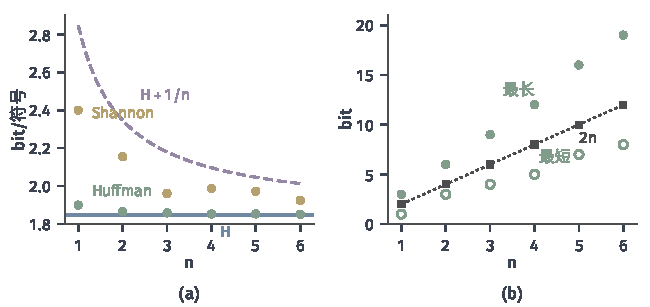
\includegraphics[width=110mm]{figures/07-probability/05-source-coding/matplotlib/lossless-block-huffman/figure.pdf}
 \caption{贯穿例的变长块编码，块长$n=1,\dots,6$。(a)每符号平均码长：绿点为块上的Huffman码，黄点为块上的Shannon码，蓝线为熵$H=1.846$，紫色虚线为上界$H+1/n$。(b)块上Huffman码的最短码字（空心绿点）与最长码字（实心绿点），灰色方点为同一块长的定长码$2n$位。}
 \label{fig:lossless-block-huffman}
\end{BookInlineFigure}

块编码对概率很不均匀的信源收益更大。第~\ref{sec:lossless-average-length}节的二元信源$\theta=0.1$，熵为$0.469$，逐符号编码至少要$1$位。块上Huffman码的每符号平均码长在$n=1,\dots,6$时为
\[
 \begin{gathered}
 1.000,\quad 0.645,\quad 0.533,\\
 0.493,\quad 0.480,\quad 0.470 ,
 \end{gathered}
\]
$n=6$时已与熵只差$0.001$位；$n=7$时反而回升到$0.474$。逐符号编码一半以上的位数是取整造成的，合成块以后这部分几乎全部收回。

\paragraph{平均保证不管最坏情形}
式~\eqref{eq:lossless-block-bound}是关于平均的。图~\ref{fig:lossless-block-huffman}(b)显示，块上Huffman码的最长码字随$n$增长得比定长码快：$n=6$时最长码字$19$位，而定长码只需$12$位；最长码字属于$dddddd$这样概率为$10^{-6}$的块。零错误的要求意味着这些罕见的块也必须有码字，它们只能放在码树的深处。

块编码的另外两项代价不在式~\eqref{eq:lossless-block-bound}中。一是码本：块上的码表有$4^n$项，$n=6$时为$4096$项，编码器与解码器都要存储，若码表要随消息一起传送，还要计入它的描述长度。二是构造与查找：Huffman构造需要$O(4^n\cdot n)$次比较。所以“块越长越接近熵”只在不计码本与计算代价时成立，第~\ref{sec:lossless-finite-resources}节把这些代价放在一起比较。

\subsection{允许错误的定长块编码}
\label{sec:lossless-fixed-block}

现在换一种要求：码字都等长，每块用同样多的位，但允许极少数块无法还原。这时问题变成“需要给多少个块编号”。四符号信源长度为$n$的块共有$4^n$个，全部编号需要$2n$位；如果绝大部分概率集中在少得多的块上，只给这些块编号就够了。

\begin{definition}[定长块编码与码率]
\label{def:lossless-fixed-length}
块长为$n$、含$M_n$个码字的定长块编码由编码映射$f_n:\mathcal{X}^n\to\{1,\dots,M_n\}$与解码映射$g_n:\{1,\dots,M_n\}\to\mathcal{X}^n$组成。每个编号用$\lceil\log_2M_n\rceil$位表示，\term{码率}（code rate）定义为
\begin{equation}
 R_n=\frac{\log_2M_n}{n}
 \label{eq:lossless-rate}
\end{equation}
单位是bit每源符号。错误概率为
\begin{equation}
 P_{\mathrm{e}}^{(n)}=\mathbb{P}\bigl(g_n(f_n(X_{1:n}))\neq X_{1:n}\bigr).
 \label{eq:lossless-error-prob}
\end{equation}
\end{definition}

\paragraph{自信息的集中}
要找出“概率集中在哪些块上”，先看一个块的每符号自信息$-\frac1n\log_2p(X_{1:n})$。由引理~\ref{lem:lossless-block-entropy}的证明，它是$n$个独立同分布随机变量
\[
 Y_i=-\log_2p(X_i)
\]
的样本平均。$Y_i$只取有限个值，均值是$H(X)$，方差
\[
 \sigma^2=\operatorname{Var}(Y_1)=\sum_xp(x)\bigl(-\log_2p(x)-H(X)\bigr)^2
\]
有限。第~\ref{chap:laws-of-large-numbers}章的弱大数律于是给出下面的结论。

\begin{theorem}[渐近均分性]
\label{thm:lossless-aep}
设$X_1,X_2,\dots$独立同分布，取值于有限字母表，各$p(x)>0$。则对每个$\varepsilon>0$，
\begin{equation}
 \mathbb{P}\Bigl(\Bigl\lvert-\frac1n\log_2p(X_{1:n})-H(X)\Bigr\rvert\geq\varepsilon\Bigr)\leq\frac{\sigma^2}{n\varepsilon^2}\xrightarrow[n\to\infty]{}0 .
 \label{eq:lossless-aep}
\end{equation}
\end{theorem}

\begin{proof}
$-\frac1n\log_2p(X_{1:n})=\frac1n\sum_iY_i$，其期望为$H(X)$，方差为$\sigma^2/n$。对它用第~\ref{chap:tail-probabilities}章的Chebyshev不等式即得。
\end{proof}

这一性质称为\term{渐近均分性}（asymptotic equipartition property）。名称的含义是：$n$大时，实际出现的块几乎都满足
\[
 p(x_{1:n})\approx2^{-nH(X)},
\]
即它们的概率“近似相等”，都在$2^{-n(H\pm\varepsilon)}$之间。这并不是说最可能的块概率接近$2^{-nH}$：贯穿例中最可能的块$aa\cdots a$的概率是$0.4^n=2^{-1.32n}$，远大于$2^{-1.85n}$；只是这样的块太少，合起来的概率可以忽略。

图~\ref{fig:lossless-aep-concentration}画出贯穿例中每符号自信息的精确分布。它按块中$a,b,c,d$的个数枚举所有类型，逐类求和得到，没有用到模拟。$n=10$时分布还很宽，落在$H\pm0.1$内的概率只有$0.337$；$n=250$时，这一概率升到$0.990$。

\begin{BookInlineFigure}
 \centering
 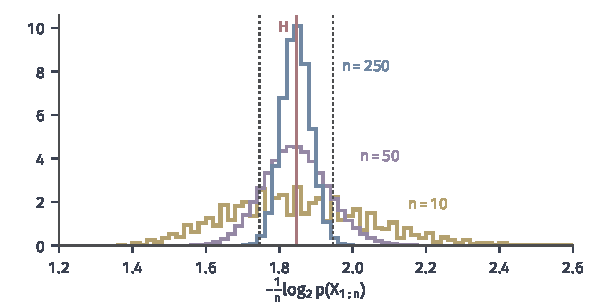
\includegraphics[width=100mm]{figures/07-probability/05-source-coding/matplotlib/lossless-aep-concentration/figure.pdf}
 \caption{贯穿例中每符号自信息$-\frac1n\log_2p(X_{1:n})$的精确分布，按宽$0.02$的格子汇总，纵轴为单位长度上的概率。黄、紫、蓝分别为$n=10,50,250$；红线为熵$H=1.846$，灰色虚线为$H\pm0.1$。}
 \label{fig:lossless-aep-concentration}
\end{BookInlineFigure}

\paragraph{典型集}
把每符号自信息接近熵的块收集起来。

\begin{definition}[典型集]
\label{def:lossless-typical-set}
对$\varepsilon>0$，称
\begin{equation}
 A_{\varepsilon}^{(n)}=\Bigl\{x_{1:n}\in\mathcal{X}^n:\ \Bigl\lvert-\frac1n\log_2p(x_{1:n})-H(X)\Bigr\rvert<\varepsilon\Bigr\}
 \label{eq:lossless-typical-set}
\end{equation}
为\term{典型集}（typical set）。
\end{definition}

等价地，$x_{1:n}\in A_{\varepsilon}^{(n)}$当且仅当
\[
 2^{-n(H(X)+\varepsilon)}<p(x_{1:n})<2^{-n(H(X)-\varepsilon)},
\]
即典型块的概率被夹在两个以熵为指数的数之间。

\begin{lemma}[典型集的性质]
\label{lem:lossless-typical-properties}
在定理~\ref{thm:lossless-aep}的条件下：
\begin{enumerate}
 \item 典型集的概率满足
 \begin{equation}
  \mathbb{P}\bigl(X_{1:n}\in A_{\varepsilon}^{(n)}\bigr)\geq1-\frac{\sigma^2}{n\varepsilon^2},
  \label{eq:lossless-typical-prob}
 \end{equation}
 从而趋于$1$；
 \item 典型集的大小满足
 \begin{equation}
  \lvert A_{\varepsilon}^{(n)}\rvert<2^{n(H(X)+\varepsilon)};
  \label{eq:lossless-typical-upper}
 \end{equation}
 \item 若典型集的概率不小于$1-\delta$，则
 \begin{equation}
  \lvert A_{\varepsilon}^{(n)}\rvert>(1-\delta)\,2^{n(H(X)-\varepsilon)}.
  \label{eq:lossless-typical-lower}
 \end{equation}
\end{enumerate}
\end{lemma}

\begin{proof}
第一条是式~\eqref{eq:lossless-aep}取补事件，即式~\eqref{eq:lossless-typical-prob}。第二条：典型集中每个块的概率都大于$2^{-n(H+\varepsilon)}$，它们的概率之和不超过$1$，所以
\[
 1\geq\sum_{x_{1:n}\in A_{\varepsilon}^{(n)}}p(x_{1:n})>\lvert A_{\varepsilon}^{(n)}\rvert\,2^{-n(H+\varepsilon)} .
\]
第三条：典型集中每个块的概率都小于$2^{-n(H-\varepsilon)}$，所以
\[
 1-\delta\leq\sum_{x_{1:n}\in A_{\varepsilon}^{(n)}}p(x_{1:n})<\lvert A_{\varepsilon}^{(n)}\rvert\,2^{-n(H-\varepsilon)} .
\]
整理即得。
\end{proof}

引理说明典型集“小而重”：它的元素个数大约是$2^{nH}$，只占全部$2^{n\log_2\lvert\mathcal{X}\rvert}$个块中的指数小部分，却几乎承载了全部概率。贯穿例中$\log_2 4=2$而$H=1.846$，比例约为
\[
 2^{-n(2-1.846)}=2^{-0.154n},
\]
$n=250$时约为$2^{-38}$。

式~\eqref{eq:lossless-typical-lower}说明上界~\eqref{eq:lossless-typical-upper}在指数上不能再改进：典型集至少要有约$2^{n(H-\varepsilon)}$个元素。图~\ref{fig:lossless-typical-set}给出$\varepsilon=0.1$时的精确数值。左图中典型集的概率随$n$上升，$n=230$时为$0.987$，远高于Chebyshev下界；右图中$\frac1n\log_2\lvert A_{\varepsilon}^{(n)}\rvert$落在$H\pm\varepsilon$之间，并明显低于$\log_24=2$。它靠近上端$H+\varepsilon$而不是$H$，是因为自信息较大的块数目多得多，典型集中的块大部分来自区间的上端。

\begin{BookInlineFigure}
 \centering
 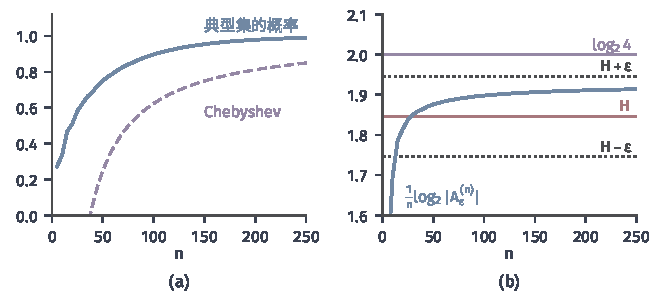
\includegraphics[width=110mm]{figures/07-probability/05-source-coding/matplotlib/lossless-typical-set/figure.pdf}
 \caption{贯穿例的典型集，$\varepsilon=0.1$，由类型枚举精确计算。(a)典型集的概率（蓝）与Chebyshev下界$1-\sigma^2/(n\varepsilon^2)$（紫色虚线），$\sigma^2=0.377$。(b)$\frac1n\log_2\lvert A_{\varepsilon}^{(n)}\rvert$（蓝），红线为$H$，灰色虚线为$H\pm\varepsilon$，紫线为全部块的$\log_24=2$。}
 \label{fig:lossless-typical-set}
\end{BookInlineFigure}

\paragraph{码率高于熵时可以做到}
典型集直接给出一种定长块编码：给典型集中的块逐个编号，另外留一个编号给所有非典型块。图~\ref{fig:lossless-typical-scheme}画出这一方案。

\begin{BookInlineFigure}
 \centering
 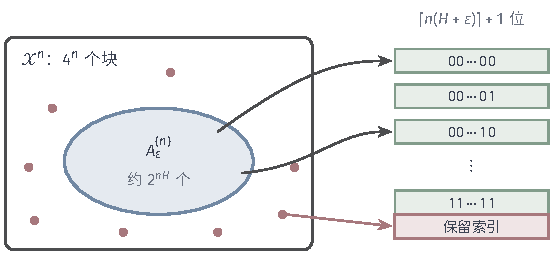
\includegraphics[width=94mm]{figures/07-probability/05-source-coding/tikz/lossless-typical-scheme/figure.pdf}
 \caption{用典型集构造定长块编码。左框为全部$4^n$个块，蓝色区域为典型集$A_{\varepsilon}^{(n)}$，约有$2^{nH}$个块；右侧绿格为等长的编号，每个典型块得到一个编号。红点为非典型块，全部送到红色的保留编号，解码时无法还原。}
 \label{fig:lossless-typical-scheme}
\end{BookInlineFigure}

\begin{theorem}[定长块编码的可达性]
\label{thm:lossless-fixed-achievability}
在定理~\ref{thm:lossless-aep}的条件下，对任意$R>H(X)$，存在一列定长块编码，其码率$R_n\leq R$（$n$充分大），错误概率$P_{\mathrm{e}}^{(n)}\to0$。
\end{theorem}

\begin{proof}
取$\varepsilon=(R-H(X))/2>0$。令编码映射把典型集中的块一一对应到编号$1,\dots,\lvert A_{\varepsilon}^{(n)}\rvert$，把其余块都映到编号$M_n=\lvert A_{\varepsilon}^{(n)}\rvert+1$；解码映射把前面的编号映回对应的典型块，把保留编号映到任意固定的块。由式~\eqref{eq:lossless-typical-upper}，
\[
 M_n<2^{n(H+\varepsilon)}+1\leq2^{n(H+2\varepsilon)}=2^{nR}
\]
在$n$充分大时成立，所以$R_n\leq R$。典型块都被正确还原，错误只可能发生在非典型块上，按式~\eqref{eq:lossless-error-prob}与式~\eqref{eq:lossless-typical-prob}，
\[
 P_{\mathrm{e}}^{(n)}\leq\mathbb{P}\bigl(X_{1:n}\notin A_{\varepsilon}^{(n)}\bigr)\leq\frac{\sigma^2}{n\varepsilon^2}\to0 . \qedhere
\]
\end{proof}

\paragraph{码率低于熵时做不到}
反过来，若码率低于熵，无论怎样选择要编号的块，错误概率都不能趋于零，实际上趋于$1$。

\begin{theorem}[定长块编码的逆定理]
\label{thm:lossless-fixed-converse}
在定理~\ref{thm:lossless-aep}的条件下，设$R<H(X)$，定长块编码满足$M_n\leq2^{nR}$。则$P_{\mathrm{e}}^{(n)}\to1$。
\end{theorem}

\begin{proof}
解码映射只有$M_n$个输出，能被正确还原的块组成集合
\[
 B_n=\{x_{1:n}:\ g_n(f_n(x_{1:n}))=x_{1:n}\},
\]
它的元素都在$g_n$的值域中，所以$\lvert B_n\rvert\leq M_n\leq2^{nR}$。取$\varepsilon=(H(X)-R)/2>0$，把正确还原的概率按是否典型拆开：
\[
 \mathbb{P}(X_{1:n}\in B_n)\leq\mathbb{P}\bigl(X_{1:n}\in B_n\cap A_{\varepsilon}^{(n)}\bigr)+\mathbb{P}\bigl(X_{1:n}\notin A_{\varepsilon}^{(n)}\bigr).
\]
第一项中每个块的概率小于$2^{-n(H-\varepsilon)}$，块的个数不超过$2^{nR}$，所以
\[
 \mathbb{P}\bigl(X_{1:n}\in B_n\cap A_{\varepsilon}^{(n)}\bigr)<2^{nR}\,2^{-n(H-\varepsilon)}=2^{-n\varepsilon}.
\]
第二项不超过$\sigma^2/(n\varepsilon^2)$。两项都趋于零，所以正确还原的概率趋于零，从而
\[
 P_{\mathrm{e}}^{(n)}=1-\mathbb{P}(X_{1:n}\in B_n)\to1. \qedhere
\]
\end{proof}

两个定理合起来说明，定长块编码能以趋于零的错误概率工作，当且仅当码率超过熵（$R=H$这一临界情形，上面的论证不作结论）。图~\ref{fig:lossless-fixed-rate-error}给出贯穿例中最好的定长码的错误概率：对给定的$M_n=\lfloor2^{nR}\rfloor$，编号给概率最大的$M_n$个块时错误概率最小。$R=1.95$时错误概率从$n=4$的$0.0157$降到$n=228$的$5.4\times10^{-5}$；$R=1.75$时，即使挑选最可能的块，错误概率仍从$0.160$升到$0.956$。

\begin{BookInlineFigure}
 \centering
 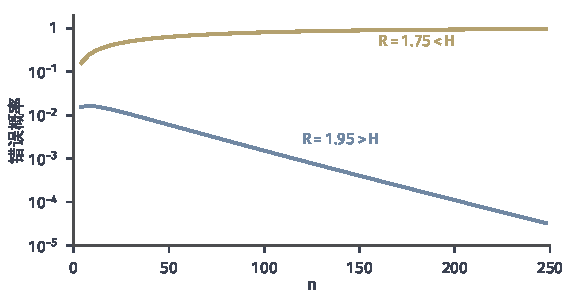
\includegraphics[width=96mm]{figures/07-probability/05-source-coding/matplotlib/lossless-fixed-rate-error/figure.pdf}
 \caption{贯穿例中码率为$R$的最优定长块编码的错误概率，纵轴为对数坐标。编码给概率最大的$\lfloor2^{nR}\rfloor$个块编号，其余块出错；数值由类型枚举精确计算。蓝线$R=1.95>H$，黄线$R=1.75<H$，$H=1.846$。}
 \label{fig:lossless-fixed-rate-error}
\end{BookInlineFigure}

\paragraph{错误来自哪里}
可达性定理中的错误全部来自非典型块，这些块合起来的概率很小。对单个块而言，结论是“要么精确还原，要么完全失败”：典型块精确还原，非典型块（例如$aa\cdots a$，以及$dd\cdots d$）一律出错。所以定理不能理解为“每条消息都能以接近熵的码率无损还原”。也不能理解为有限的$n$下错误概率已经可以忽略：贯穿例中$R=1.95$、$n=100$时错误概率仍有$1.5\times10^{-3}$。需要每条消息都还原时，应当用上一小节的变长块编码，它把这些罕见的块放到很长的码字里，而不是放弃它们。


\section{有限资源下的比较}
\label{sec:lossless-finite-resources}

前面的极限都在$n\to\infty$时成立，并且假定编码器知道真实的分布。实际选择编码方案时，块长有限，模型可能不准，码表要存储，编码要计算。本节在贯穿例上把各种方案放在同一组条件下比较：源分布相同，按每个源符号计算码长，解码要求分别写明。

\paragraph{几种方案的账本}
表~\ref{tab:lossless-comparison}列出贯穿例上的几种方案。平均码长一栏都按每源符号计；“最长码字”按一个编码单位（一个符号、一个块或整条消息）计；码本一栏是编码器与解码器需要共享的表的规模。

\begin{BookInlineTable}
 \centering
 \caption{贯穿例$p=(0.4,0.3,0.2,0.1)$上的几种编码方案，$H=1.846$。算术编码一行为图~\ref{fig:lossless-arith-length}中长$400$、长度已知的那条消息的实测值，码长小于消息自信息加$2$；定长块一行为图~\ref{fig:lossless-fixed-rate-error}中$R=1.95$、$n=100$的最优定长码。}
 \label{tab:lossless-comparison}
 \begin{tabular}{lcccc}
  \toprule
  方案 & 位/符号 & 最长码字 & 共享的表 & 错误概率\\
  \midrule
  定长$2$位 & $2$ & $2$ & 无 & $0$\\
  Huffman，$n=1$ & $1.900$ & $3$ & $4$项 & $0$\\
  Huffman，$n=2$ & $1.865$ & $6$ & $16$项 & $0$\\
  Huffman，$n=4$ & $1.853$ & $12$ & $256$项 & $0$\\
  Huffman，$n=6$ & $1.851$ & $19$ & $4096$项 & $0$\\
  算术编码 & $1.855$ & 随消息 & $4$个概率 & $0$\\
  定长块 & $1.95$ & $195$ & 排序规则 & $0.0015$\\
  \bottomrule
 \end{tabular}
\end{BookInlineTable}

从表中可以读出三点。第一，从$n=1$到$n=6$，块上Huffman码每符号只省下$0.049$位，码表却从$4$项增长到$4096$项，最长码字从$3$位增长到$19$位：越接近熵，每一点改进越贵。第二，算术编码只需共享四个概率，就达到了与$n=6$的块Huffman码相当的每符号码长；代价是每个符号要做乘法和区间比较，并且要处理有限精度。第三，定长块编码的码字最整齐，但要接受正的错误概率，不能用于必须逐条还原的场合。

\paragraph{码本的描述代价}
若编码器与解码器事先没有共享码表，码表本身也要传送。Huffman码由码长完全决定：把码长按从短到长排好，用第~\ref{sec:lossless-kraft}小节Kraft不等式充分性证明中的方法分配码字，得到的前缀码称为规范码，解码器只需知道每个块的码长。块长为$n$时要传送$4^n$个码长，每个码长用几位表示，总共是$4^n$乘以一个常数的位数。若消息只有$N$个符号，这一开销摊到每个符号上是$4^n/N$量级，块长增大带来的不到$1/n$位的收益，很快被它抵消。算术编码只需传送模型的四个概率（或模型的更新规则），描述代价与块长无关。

\paragraph{计算代价}
块上Huffman码的构造需要对$4^n$个块排序合并，计算量$O(4^n\cdot n)$；编码时查表，解码时在码树上逐位行走。算术编码不需要构造码表，每读一个符号做常数次乘法与比较，解码时要在累积概率表中找到$v$所在的子区间，字母表较大时用二分查找。两者都是每个源符号常数量级的工作，但Huffman码的常数随块长指数增长，算术编码的常数与消息长度无关。

\paragraph{模型失配的代价}
设计编码时用的分布$q$称为模型，信源的真实分布是$p$，两者可能不同。码长是按$q$设计的，平均码长却要按实际出现的频率，即按$p$加权。定理~\ref{thm:lossless-entropy-bound}证明中的分解在这里给出精确的账目。

\begin{theorem}[失配的Shannon码]
\label{thm:lossless-mismatch}
设$p,q$是$\mathcal{X}$上的概率质量函数，各$p(x)>0$、$q(x)>0$，且$q(x)<1$对每个$x$成立。按模型$q$取码长$\ell(x)=\lceil-\log_2q(x)\rceil$的前缀码，在真实分布$p$下的平均码长满足
\begin{equation}
 H(p)+D_{\mathrm{KL}}(p\Vert q)\leq\sum_xp(x)\ell(x)<H(p)+D_{\mathrm{KL}}(p\Vert q)+1 ,
 \label{eq:lossless-mismatch}
\end{equation}
其中$H(p)$是$p$的熵。
\end{theorem}

\begin{proof}
码长满足Kraft不等式，理由同定理~\ref{thm:lossless-entropy-bound}，所以这样的前缀码存在。对每个$x$，
\[
 -\log_2q(x)=-\log_2p(x)+\log_2\frac{p(x)}{q(x)} .
\]
按$p$加权求和，右边的平均是$H(p)+D_{\mathrm{KL}}(p\Vert q)$。而$-\log_2q(x)\leq\ell(x)<-\log_2q(x)+1$，乘$p(x)$求和即得式~\eqref{eq:lossless-mismatch}。
\end{proof}

所以模型失配的代价是KL散度$D_{\mathrm{KL}}(p\Vert q)$：按错误的概率分配码长，每符号平均多付这么多位。左侧的不等式说明这部分损失无法靠取整挽回；它与整数码长的冗余是两笔不同的账。

图~\ref{fig:lossless-mismatch}在贯穿例上让模型从$p$逐渐变到反序的$r=(0.1,0.2,0.3,0.4)$，即$q_t=(1-t)p+tr$。$t=0$时模型准确，Huffman码平均$1.9$位；$t=1$时按$r$设计的Huffman码给$a$三位、$d$一位，按真实概率加权，
\[
 0.4\times3+0.3\times3+0.2\times2+0.1\times1=2.6 ,
\]
比准确模型多$0.7$位，比定长码还差。此时$D_{\mathrm{KL}}(p\Vert r)=0.658$，Shannon码平均$3.1$位，落在式~\eqref{eq:lossless-mismatch}给出的$[2.505,3.505)$中。另一个特例是均匀模型：码长都是$2$，平均码长$2$恰好等于
\[
 H(p)+D_{\mathrm{KL}}(p\Vert u)=1.846+0.154 .
\]

\begin{BookInlineFigure}
 \centering
 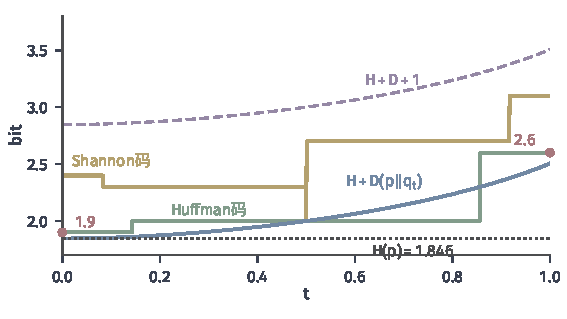
\includegraphics[width=96mm]{figures/07-probability/05-source-coding/matplotlib/lossless-mismatch/figure.pdf}
 \caption{模型失配。真实分布$p=(0.4,0.3,0.2,0.1)$，设计模型$q_t=(1-t)p+t\,r$，$r=(0.1,0.2,0.3,0.4)$。纵轴为按$p$计算的平均码长：黄线为按$q_t$设计的Shannon码，绿线为按$q_t$设计的Huffman码；蓝线为$H(p)+D_{\mathrm{KL}}(p\Vert q_t)$，紫色虚线为再加$1$，灰色点线为$H(p)$。红点为两端的Huffman码平均码长。}
 \label{fig:lossless-mismatch}
\end{BookInlineFigure}

图中Huffman码的曲线是阶梯形：模型稍有偏差时，码长的整数取值往往不变，平均码长也不变；偏差累积到改变码树时才跳一级。在$t$约从$0.5$到$0.86$之间，按$q_t$设计的Huffman码甚至落在蓝线下方，这并不矛盾：式~\eqref{eq:lossless-mismatch}只约束Shannon码，任何码的平均码长只受$H(p)$约束。

\paragraph{失配与不一致是两回事}
模型失配时，编码器与解码器用同一个$q$，码仍然唯一可译，每条消息都正确还原，只是平均更长。另一种错误是两端不一致：编码器与解码器用了不同的码表或不同的概率。这时码长没有变，解码结果却错了。

两个例子都来自本章的码表。第~\ref{sec:lossless-model}节的码表中$c\mapsto110$、$d\mapsto111$，第~\ref{sec:lossless-huffman}小节Huffman过程得到的码表中$c\mapsto111$、$d\mapsto110$，两者平均码长相同。若编码器用前者把$abac$编成$0100110$，解码器却用后者，读出的是$abad$。算术编码也一样：编码器按$p=(0.4,0.3,0.2,0.1)$把$abac$编成$00110010$，若解码器误用$(0.3,0.4,0.2,0.1)$，则从$v=0.1953$逐步读出
\[
 a,\quad b,\quad c,\quad c ,
\]
得到$abcc$。

所以评价一个方案要分开两件事：在两端一致的前提下，模型偏离真实分布会使平均码长增加$D_{\mathrm{KL}}(p\Vert q)$左右；两端不一致则破坏可解码性，与平均码长无关。前者靠更好的模型改进，后者要靠严格共享的规则（码长表、符号顺序、概率与取整方式）来避免。


\section{本章小结}
\label{sec:lossless-summary}

本章从“常见符号用短码能省多少”出发，回答了三个层次的问题，每个层次对应各自的约束。

第一层是可解码性。码字互不相同还不够，拼接以后必须能唯一地切开。前缀码让解码器在码树上即时断开码字；唯一可译码允许码字互为前缀，但要付出解码延迟。Kraft–McMillan不等式说明两者能实现的码长集合相同，都由$\sum_x2^{-\ell(x)}\leq1$刻画；这一条件约束的是码长，码字仍须按保证前缀性的方法分配。

第二层是平均码长的最优性。对至少两个符号有正概率的信源，唯一可译码的平均码长不小于熵，等号要求每个码长恰为自信息；按自信息取整的Shannon码平均码长小于熵加一。平均码长与熵之差拆成两部分：码长暗含的概率与真实概率的KL散度，以及Kraft不等式未取等号所浪费的空间。冗余是加权平均，个别符号的码长可以短于自信息。确定源只有在消息长度已知时才能零码长。

第三层是可执行的构造与渐近极限。Huffman编码逐次合并概率最小的两个符号，对给定有限符号表求出平均码长最短的前缀码，贯穿例中为$1.9$位，熵为$1.846$位。

算术编码把整条消息对应到长度等于其概率的区间，码长不超过自信息加两位，需要约定终止规则，两端须使用完全相同的模型与取整方式，模型给实际符号零概率时无法编码。

把符号组成块之后有两种资源制度：零错误的变长块编码使每符号冗余小于$1/n$，代价是最坏码长和码本随块长增长；允许错误的定长块编码借助渐近均分性和典型集，码率高于熵时错误概率趋于零，低于熵时趋于一，失败来自被放弃的小概率块。

在有限资源下，块长带来的收益很快被码本与计算代价抵消；模型失配使平均码长增加KL散度，两端不一致则直接造成解码错误。第~\ref{chap:quantization}章不再要求精确还原，允许重构值与原值有偏差，研究把连续取值装进有限个格子的量化器，并用失真来衡量这种偏差；量化后的格子编号仍可用本章的方法无损压缩。


\chapter{量化}
\label{chap:quantization}

一个传感器读出的是实数，例如某个零件尺寸偏离标称值的毫米数。它服从密度为$f(x)=\tfrac12\mathrm{e}^{-\lvert x\rvert}$的Laplace分布$\operatorname{Laplace}(0,1)$：多数读数靠近零，偶尔出现较大的偏差。若每个读数只允许存2个比特，也就是只能记录4种结果之一，那么这4个代表值应当放在哪里？哪些读数归给哪个代表值？这样记录后，平均要付出多大的平方误差？

第~\ref{chap:lossless-coding}章要求接收者精确还原每个符号。连续取值做不到这一点：实数轴的任意一个区间里都有不可数多个数，而有限长的二进制串一共只有可数多个，任何有限描述都必须把许多不同的读数合并成同一个结果。合并会带来误差，问题变成在给定的描述资源下怎样合并，使误差尽量小。

本章先把这件事写成模型：把取值空间分成有限个区域，每个区域配一个重构值，再用源分布和失真函数计算平均代价，并分清点数、定长索引和压缩后索引长度这三种资源。随后构造标量量化器：等距划分最容易实现，按分布调整的划分则由“固定区域选代表、固定代表选区域”的交替改进得到。

接着把同样的两条条件推广到向量，说明联合码本怎样利用分量之间的相关性和区域形状，又要付出怎样的存储与搜索代价。量化器确定以后，区域索引是一个离散随机变量，可以用上一章的方法再压缩，这一步改变平均描述长度而不改变重构结果；若要把码长也一起优化，目标函数就要改写。最后分析误差本身：有限范围造成的过载、范围内的舍入，以及加入共享随机扰动之后误差与输入的关系怎样改变。

全章以上述Laplace读数为贯穿例子，多数数值可以手算。所用的期望、条件期望与方差分解来自第~\ref{chap:random-variable-moments}章和第~\ref{chap:conditional-expectation}章，熵与平均码长来自第~\ref{chap:information-measures}章和第~\ref{chap:lossless-coding}章。本章对数以$2$为底，描述长度以bit计。

\section{量化模型}
\label{sec:quant-model}

记录一个连续读数，最朴素的做法是规定一组刻度，把读数报成离它最近的刻度。温度计只标到$0.1$度，读数$20.03$和$20.04$都记成$20.0$。这已经包含了量化的全部要素：哪些读数被合并到一起，合并后报出哪个值，合并造成多大的差。下面先把这三件事分开写成数学对象，再规定怎样计算平均误差、怎样计量所用的描述资源。

\paragraph{区域、索引与重构值}

可以把量化想成把读数装进有限个抽屉：每个抽屉占取值空间的一块区域，读数落进哪块区域就放进哪个抽屉；记录时只写抽屉的编号，取用时每个编号对应一个事先约定的代表值。与温度计刻度不同，抽屉的边界和代表值都由我们来选，代表值也不必位于区域的正中。这个类比在一处会失效：抽屉里的东西还能取出来，而量化后只剩编号，同一区域内的不同读数已经无法区分。

取值空间记为$\mathbb{R}^{d}$，$d=1$是单个读数，$d\geq2$是几个读数一起处理。区域要能计算概率，所以要求它们是Borel集；在第~\ref{chap:probability-spaces}章的意义下，这保证了$\mathbb{P}(\bm{X}\in S_j)$有定义。

\begin{definition}[量化器]
\label{def:quant-quantizer}
设$N\geq1$为整数。取值空间$\mathbb{R}^{d}$上的一个$N$点\term{量化器}（quantizer）$Q$由两部分组成：一组两两不交、并集为$\mathbb{R}^{d}$的Borel集$S_1,\dots,S_N$，称为它的区域；以及$N$个点$\bm{c}_1,\dots,\bm{c}_N\in\mathbb{R}^{d}$，称为\term{重构值}（reconstruction value），全体$\mathcal{C}=\{\bm{c}_1,\dots,\bm{c}_N\}$称为\term{码本}（codebook）。编码器与解码器分别是
\begin{equation}
 \alpha(\bm{x})=j\quad(\bm{x}\in S_j),\qquad \beta(j)=\bm{c}_j ,
 \label{eq:quant-encoder-decoder}
\end{equation}
量化器是二者的复合$Q(\bm{x})=\beta(\alpha(\bm{x}))$。
\end{definition}

编码器$\alpha$只输出区域的编号，称为\term{量化索引}（quantization index）；解码器$\beta$只看编号，不知道原来的读数。因此$Q$在每个区域上取常值，它的值域至多有$N$个点。对随机输入$\bm{X}$，索引$J=\alpha(\bm{X})$是取值于$\{1,\dots,N\}$的离散随机变量，概率质量为
\begin{equation}
 p_j=\mathbb{P}(J=j)=\mathbb{P}(\bm{X}\in S_j),\qquad j=1,\dots,N .
 \label{eq:quant-index-pmf}
\end{equation}

区域之间的边界点归哪一侧，需要事先约定。对有密度的输入，边界通常是概率为零的集合，约定不影响平均误差；对离散输入，边界上可能有正的概率，约定会改变结果，后面遇到时再说明。

\paragraph{失真与平均失真}

合并的代价用一个非负函数衡量：读数为$\bm{x}$而报出$\hat{\bm{x}}$时，代价是$d(\bm{x},\hat{\bm{x}})\geq0$，称为\term{失真函数}（distortion function），要求它是Borel可测的。本章主要使用平方误差
\begin{equation}
 d(\bm{x},\hat{\bm{x}})=\lVert\bm{x}-\hat{\bm{x}}\rVert_2^2 ,
 \label{eq:quant-squared-error}
\end{equation}
标量情形就是$(x-\hat{x})^2$。平方误差对大偏差惩罚更重，并且能和期望、方差的运算直接配合，下一节会反复用到这一点。

单个读数的失真是随机的，评价量化器时取它的平均。

\begin{definition}[平均失真]
\label{def:quant-average-distortion}
设$\bm{X}$的分布为$P_{\bm{X}}$，$Q$是由区域$S_j$和重构值$\bm{c}_j$给出的量化器。$Q$的\term{平均失真}（average distortion）是
\begin{equation}
 D(Q)=\mathbb{E}\bigl[d(\bm{X},Q(\bm{X}))\bigr]=\sum_{j=1}^{N}\int_{S_j}d(\bm{x},\bm{c}_j)\,P_{\bm{X}}(\mathrm{d}\bm{x}) .
 \label{eq:quant-average-distortion}
\end{equation}
它是非负可测函数的期望，总有定义，可能为$+\infty$。
\end{definition}

式~\eqref{eq:quant-average-distortion}的第二个等号把期望按区域拆开：在$S_j$上$Q$恒等于$\bm{c}_j$，所以每块只是一个普通的积分。对平方误差，只要$\mathbb{E}[\lVert\bm{X}\rVert_2^2]<\infty$，平均失真对任何码本都有限，因为
\[
 \lVert\bm{x}-\bm{c}_j\rVert_2^2\leq2\lVert\bm{x}\rVert_2^2+2\lVert\bm{c}_j\rVert_2^2 .
\]
本章讨论平方误差时都假定输入的二阶矩有限。

平均失真同时依赖三样东西：源分布、区域划分和重构值。源分布是给定的，后两者由设计者选择。“好的量化器”永远是相对于某个源分布和某个失真函数而言的，换一个分布，同一个量化器的平均失真就会改变。

\paragraph{两点量化器}
用本章开头的Laplace读数$X\sim\operatorname{Laplace}(0,1)$走一遍。只允许两个重构值时，按符号分成两个区域，配上对称的两个点：
\[
 S_1=(-\infty,0),\quad S_2=[0,\infty),\qquad c_1=-1,\quad c_2=1 .
\]
例如读数$x=0.7$落在$S_2$，编码器输出$j=2$，解码器报出$c_2=1$，误差是$0.3$。

计算平均失真时，由对称性，两个区域贡献相同，只需算$S_2$。在$X\geq0$的条件下，$X$服从$\operatorname{Exp}(1)$，第~\ref{chap:common-distributions}章给出它的一、二阶矩
\[
 \mathbb{E}[X\mid X\geq0]=1,\qquad \mathbb{E}[X^{2}\mid X\geq0]=2 .
\]
把平方展开，得到
\[
 \mathbb{E}\bigl[(X-1)^{2}\mid X\geq0\bigr]=2-2\cdot1+1=1 .
\]
两个区域各占概率$\tfrac12$，于是
\[
 D(Q)=\tfrac12\cdot1+\tfrac12\cdot1=1 .
\]

作为对照，如果什么都不记录，只能对所有读数报同一个常数$c$。平方误差$\mathbb{E}[(X-c)^2]$在$c=\mathbb{E}[X]=0$时最小，最小值是$\operatorname{Var}(X)=2$。一个比特把平均失真从$2$降到$1$。图~\ref{fig:quant-two-points}画出了这个量化器：左图是两个区域与重构值在密度上的位置，右图是映射$Q(x)$本身，它是一条只取两个值的阶梯，与对角线$y=x$的竖直距离就是误差。

\begin{BookInlineFigure}
 \centering
 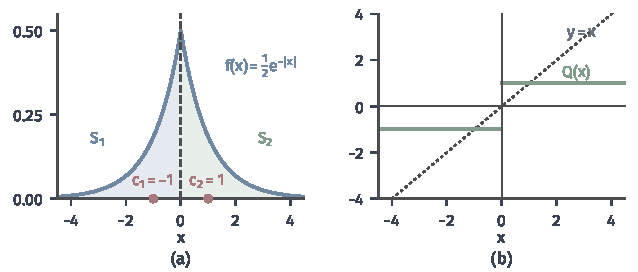
\includegraphics[width=108mm]{figures/07-probability/05-source-coding/matplotlib/quant-two-points/figure.pdf}
 \caption{$\operatorname{Laplace}(0,1)$读数的两点量化器。(a) 蓝线为密度$f$，浅蓝与浅绿分别是区域$S_1=(-\infty,0)$与$S_2=[0,\infty)$，红点为重构值$c_1=-1$、$c_2=1$，虚线为区域边界。(b) 绿线为$Q(x)$，点线为$y=x$；同一横坐标处二者的竖直距离就是误差。}
 \label{fig:quant-two-points}
\end{BookInlineFigure}

最好的重构值依赖于失真函数。若改用绝对误差$d(x,\hat{x})=\lvert x-\hat{x}\rvert$，一个区域内最好的代表值不再是条件均值，而是条件中位数：均值使平方误差最小，中位数使绝对误差最小。在$X\geq0$的条件下，$\operatorname{Exp}(1)$的中位数是$\ln2\approx0.693$，对$Z\sim\operatorname{Exp}(1)$与$c\geq0$直接积分得
\[
 \mathbb{E}\lvert Z-c\rvert=c-1+2\mathrm{e}^{-c} .
\]
取$c=\ln2$得平均绝对误差$0.693$，取$c=1$得$0.736$。同一个源、同样的两个区域，换一个失真函数，最好的重构值就从$\pm1$移到了$\pm0.693$。

右图也显示了误差的两个特点。读数靠近$\pm1$时误差小，远离时误差随$\lvert x\rvert$线性增长；误差完全由读数决定，没有任何随机性。第~\ref{sec:quant-error}节会专门分析这两点。

\paragraph{描述资源}

量化减少了需要记录的内容，但“减少了多少”有三种不同的计量方法，混用会得出错误的比较。图~\ref{fig:quant-pipeline}把一次记录拆成几个环节：编码器把读数变成索引，索引可以原样写成定长比特串，也可以先经过一次无损编码再传送，接收端恢复索引后由解码器报出重构值。

\begin{BookInlineFigure}
 \centering
 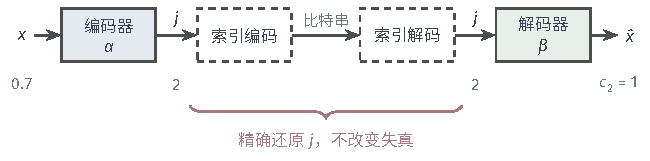
\includegraphics[width=110.1mm]{figures/07-probability/05-source-coding/tikz/quant-pipeline/figure.pdf}
 \caption{量化记录的各个环节。实线框是量化器本身：编码器$\alpha$输出区域索引$j$，解码器$\beta$报出重构值；虚线框是可选的索引编码与解码。下方灰字是两点量化器的例子：读数$0.7$得到索引$2$，重构为$c_2=1$。中间两个环节精确还原索引，因此不改变失真。}
 \label{fig:quant-pipeline}
\end{BookInlineFigure}

第一种计量是重构点数$N$，它决定量化器能区分多少种结果。第二种是\emph{定长索引长度}：每个索引都用同样多的比特写出，需要$\lceil\log_2N\rceil$个比特；$N$是$2$的幂时恰为$\log_2N$。第三种是\emph{平均索引长度}：把索引$J$看作一个离散信源，用第~\ref{chap:lossless-coding}章的唯一可译码描述它，平均长度不小于索引的熵
\[
 H(J)=-\sum_{j=1}^{N}p_j\log_2p_j ,
\]
又可以做到小于$H(J)+1$。由于$H(J)\leq\log_2N$，平均索引长度可以明显短于定长索引长度，尤其当各区域的概率很不均匀时。

处理向量时还要说清是按什么计算的。$d$个读数组成一个向量、用$N$个重构点描述时，每个向量用$\log_2N$个比特，折合每个分量
\begin{equation}
 R=\frac{1}{d}\log_2N
 \label{eq:quant-rate-per-component}
\end{equation}
个比特。比较一个标量量化器和一个二维量化器时，应当在相同的每分量比特数下比较，而不是在相同的点数下比较。

\begin{BookInlineTable}
 \centering
 \begin{tabular}{lll}
  \toprule
  资源 & 计量 & 两点量化器\\
  \midrule
  重构点数 & $N$ & $2$\\
  定长索引长度 & $\lceil\log_2N\rceil$ & $1$ bit\\
  平均索引长度 & 不小于$H(J)$ & $1$ bit\\
  \bottomrule
 \end{tabular}
 \caption{三种描述资源。两点量化器的两个区域概率都是$\tfrac12$，三种计量恰好一致；区域概率不均匀时，平均索引长度可以小于定长索引长度。}
 \label{tab:quant-resources}
\end{BookInlineTable}

表~\ref{tab:quant-resources}汇总了这三种计量。它们回答不同的问题：点数决定重构的精细程度，定长长度适合每个读数必须占用固定存储的场合，平均长度适合可以变长记录的场合。第~\ref{sec:quant-index-coding}节将看到，固定点数时用变长记录可以节省长度，而若以平均长度为预算，最优的区域划分也会随之改变。

\paragraph{有限量化器与长块极限}

给定源分布、失真函数、维数$d$和点数$N$，所有$N$点量化器中平均失真的下确界
\[
 D_N^{*}=\inf_{Q:\,N\text{点}}D(Q)
\]
是有限量化所能达到的最好水平。它依赖于一次联合处理多少个读数。同样是每个读数1 bit，逐个读数用两点量化器，与把两个读数作为二维向量用四点量化器，后者的选择范围包含前者（取两个两点量化器的乘积即可），因此不会更差，往往还更好；第~\ref{sec:quant-vector}节会给出具体例子。

把越来越长的读数块放在一起描述，每分量的最低失真还会继续下降。第~\ref{chap:rate-distortion}章研究这一极限：对方差为$\sigma^{2}$的高斯读数，允许任意长的块时，每个读数1 bit可以把均方误差降到$\sigma^{2}/4$，而逐个读数的最好两点量化器（阈值为零、重构值为$\pm\sigma\sqrt{2/\pi}$）只能达到$(1-2/\pi)\sigma^{2}\approx0.363\sigma^{2}$。所以本章算出的有限量化器失真，是具体方案在给定维数和点数下的表现，不等于给定码率下所有长块编码的最小失真；两者的差距正是下一章要衡量的量。


\section{标量量化}
\label{sec:quant-scalar}

先处理单个实值读数，$d=1$。实轴上最自然的区域是区间：取阈值
\[
 -\infty=t_0<t_1<\dots<t_{N-1}<t_N=+\infty ,
\]
令$S_j=[t_{j-1},t_j)$，再在每个区间里放一个重构值$c_j$。编码器只要把读数与阈值逐个比较，就能确定它落在哪个区间。这样的量化器称为\term{标量量化}（scalar quantization）。

区间怎么划、重构值放在哪里，有两种思路。一种是不看分布，直接按等距刻度划分，构造和编码都最简单；另一种是按源分布调整，概率集中的地方划得细，稀疏的地方划得粗。对平方误差，后一种思路可以拆成两个各自容易求解的子问题：区间固定时重构值放在哪里最好，重构值固定时区间边界放在哪里最好。轮流求解这两个子问题，就得到第~\ref{sec:quant-nonuniform}节的迭代。

\subsection{均匀量化}
\label{sec:quant-uniform}

等距划分需要先规定三件事：表示范围$[-L,L]$、重构点数$N$，以及范围外的读数怎样处理。范围被等分为$N$段，步长为
\[
 \Delta=\frac{2L}{N} .
\]

\paragraph{区间与重构值}
第$j$段区间的左右端点是$-L+(j-1)\Delta$和$-L+j\Delta$，重构值取它的中点。内部阈值和重构值分别为
\begin{equation}
 t_j=-L+j\Delta\ (j=1,\dots,N-1),\qquad c_j=-L+\bigl(j-\tfrac12\bigr)\Delta\ (j=1,\dots,N).
 \label{eq:quant-uniform-points}
\end{equation}
范围外的读数归入最外侧的区间：$x<-L$报$c_1$，$x\geq L$报$c_N$。这种约定称为\term{饱和}（saturation），相当于把两端的区间延长到无穷。于是编码器可以写成一个公式，
\begin{equation}
 \alpha(x)=\min\Bigl\{N,\ \max\Bigl\{1,\ \Bigl\lfloor\frac{x+L}{\Delta}\Bigr\rfloor+1\Bigr\}\Bigr\} ,
 \label{eq:quant-uniform-encoder}
\end{equation}
内层的取整给出读数在第几段，外层的$\max$与$\min$实现饱和。解码器按式~\eqref{eq:quant-uniform-points}查出$c_{\alpha(x)}$。这样构造的量化器称为\term{均匀量化}（uniform quantization）。

式~\eqref{eq:quant-uniform-points}中相邻重构值的中点恰好是阈值，所以在每个读数处，均匀量化器报出的都是离它最近的重构值。点数$N$为偶数时，零是阈值而不是重构值，读数在零附近时报$\pm\Delta/2$；若希望零本身是重构值，可以把刻度平移半个步长，取$c=k\Delta$，这样的量化器在第~\ref{sec:quant-dither}节使用。

\paragraph{一个编码与重构的例子}
取$N=8$、$L=4$，步长$\Delta=1$，重构值为$\pm0.5,\pm1.5,\pm2.5,\pm3.5$，每个索引用$3$个比特。下面检验三个读数。

读数$x=1.3$在范围内，$\lfloor5.3\rfloor+1=6$，于是
\[
 \alpha(1.3)=6,\qquad Q(1.3)=c_6=-4+5.5=1.5 ,
\]
误差为$0.2$。读数$x=-0.2$同样在范围内，$\lfloor3.8\rfloor+1=4$，
\[
 \alpha(-0.2)=4,\qquad Q(-0.2)=c_4=-0.5 ,
\]
误差为$-0.3$。

读数$x=5.7$超出了范围。$\lfloor9.7\rfloor+1=10$，被$\min$截到$8$，
\[
 \alpha(5.7)=8,\qquad Q(5.7)=c_8=3.5 ,
\]
误差为$-2.2$，远大于半个步长。图~\ref{fig:quant-uniform-staircase}把$Q$画成阶梯，三个读数的误差是红色竖线的长度。

\begin{BookInlineFigure}
 \centering
 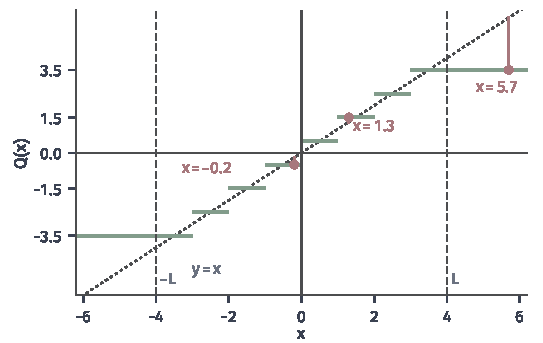
\includegraphics[width=92mm]{figures/07-probability/05-source-coding/matplotlib/quant-uniform-staircase/figure.pdf}
 \caption{$N=8$、$L=4$、$\Delta=1$的均匀量化器。绿线为阶梯$Q(x)$，点线为$y=x$，虚线标出表示范围的两端。红点是读数$1.3$、$-0.2$、$5.7$的输出，红色竖线的长度是误差；范围外的阶梯无限延长，误差随读数线性增大。}
 \label{fig:quant-uniform-staircase}
\end{BookInlineFigure}

\paragraph{有限范围的两种误差}
图中可以分出两种情形。读数在$[-L,L]$内时，它与所在区间的中点相距不超过半个步长，
\[
 \lvert x-Q(x)\rvert\leq\frac{\Delta}{2},\qquad \lvert x\rvert\leq L ;
\]
这部分误差称为\term{舍入误差}（granular error）。读数超出范围时，误差为$\lvert x\rvert-(L-\Delta/2)$，随读数无限增大，称为\term{过载误差}（overload error）。

只要$N$有限而区间都有界，就覆盖不了整条实轴，总要对范围外的读数作某种约定。饱和是最简单的一种。另一种做法是保留一个“越界”索引，再另外描述越界的读数，这等于增加了点数或改变了索引长度，比较时要把这部分资源计入。

两种误差对步长的要求相反。$N$固定时，缩小步长使舍入误差变小，却使范围$L=N\Delta/2$变窄、过载更频繁。对Laplace读数取$N=4$、$\Delta=1$，即$L=2$，重构值为$\pm0.5,\pm1.5$，平均失真为$0.5142$；第~\ref{sec:quant-granular-overload}节将把它分解成两部分，并给出权衡的方法。这个四点量化器也是下一小节迭代的起点。

\subsection{非均匀量化}
\label{sec:quant-nonuniform}

Laplace读数集中在零附近，尾部却延伸得很远。均匀刻度在这里有些浪费：中间密集的地方和尾部稀疏的地方用同样的步长。直观上，概率大的地方应当划得细些，概率小的地方划得粗些。下面固定点数$N$和平方误差，寻找使平均失真最小的区间和重构值。这样构造的量化器一般不等距，称为\term{非均匀量化}（non-uniform quantization）。

同时优化$N-1$个阈值和$N$个重构值并不容易，因为目标对它们的依赖相互纠缠。把变量分成两组，每次固定一组优化另一组，两个子问题都有显式解。

\paragraph{固定区间选重构值}
区间固定后，平均失真按区间拆成互不相关的几块，每块只依赖一个重构值，可以分别优化。于是问题化为：在一个区间上放一个点，使该区间内的平方误差最小。

期望是质量分布的重心，方差是绕重心的转动惯量。把区间$S$上的那部分概率质量看作一块物体，平方误差$\mathbb{E}[(X-c)^2\mathbf{1}_{\{X\in S\}}]$就是它绕点$c$的转动惯量，最好的$c$应当是这块质量的重心。下面的引理把这个直观写成恒等式，它是力学中平行轴定理的概率版本。

\begin{lemma}[质心条件]
\label{lem:quant-centroid}
设$\mathbb{E}[X^{2}]<\infty$，$S$是Borel集且$p=\mathbb{P}(X\in S)>0$，记条件均值
\begin{equation}
 m=\mathbb{E}[X\mid X\in S]=\frac{\mathbb{E}[X\mathbf{1}_{\{X\in S\}}]}{p} .
 \label{eq:quant-conditional-mean}
\end{equation}
则对每个实数$c$，
\begin{equation}
 \mathbb{E}\bigl[(X-c)^{2}\mathbf{1}_{\{X\in S\}}\bigr]=\mathbb{E}\bigl[(X-m)^{2}\mathbf{1}_{\{X\in S\}}\bigr]+p\,(m-c)^{2} .
 \label{eq:quant-parallel-axis}
\end{equation}
因此该区间内的平方误差在$c=m$时唯一地取到最小。
\end{lemma}

\begin{proof}
把$X-c$写成$(X-m)+(m-c)$，平方后展开：
\[
 (X-c)^{2}=(X-m)^{2}+2(m-c)(X-m)+(m-c)^{2} .
\]
两边乘$\mathbf{1}_{\{X\in S\}}$再取期望。二阶矩有限保证每一项都可积。交叉项中，
\[
 \mathbb{E}\bigl[(X-m)\mathbf{1}_{\{X\in S\}}\bigr]=\mathbb{E}[X\mathbf{1}_{\{X\in S\}}]-mp=0 ,
\]
最后一步用了式~\eqref{eq:quant-conditional-mean}。常数项的期望是$p(m-c)^{2}$，于是得到式~\eqref{eq:quant-parallel-axis}。右边第一项与$c$无关，第二项非负且只在$c=m$时为零，所以最小点唯一。
\end{proof}

式~\eqref{eq:quant-parallel-axis}说明，重构值偏离重心的代价是区间概率乘以偏离距离的平方，且与区间内部的分布形状无关。满足这一条件的重构值称为区间的质心。

用第~\ref{chap:conditional-expectation}章的语言，若每个正概率区间的重构值都是质心，则$Q(X)=\mathbb{E}[X\mid J]$，即量化输出是读数在“只知道索引”这一信息下的条件期望，也就是$X$到索引所生成的信息上的正交投影。正交性给出一个计算平均失真的捷径：
\begin{equation}
 D(Q)=\mathbb{E}[X^{2}]-\mathbb{E}\bigl[Q(X)^{2}\bigr]=\mathbb{E}[X^{2}]-\sum_{j=1}^{N}p_jc_j^{2} .
 \label{eq:quant-centroid-distortion}
\end{equation}
它由勾股定理
\[
 \mathbb{E}[X^{2}]=\mathbb{E}\bigl[Q(X)^{2}\bigr]+\mathbb{E}\bigl[(X-Q(X))^{2}\bigr]
\]
得到，只在重构值都是质心时成立。

以Laplace读数为例，看区间$[0,1)$。按$\operatorname{Laplace}(0,1)$的密度直接积分，得到这个区间的概率与一阶矩：
\[
 p=\frac{1-\mathrm{e}^{-1}}{2}=0.3161,\qquad \mathbb{E}[X\mathbf{1}_{\{0\leq X<1\}}]=\frac{1-2\mathrm{e}^{-1}}{2}=0.1321 .
\]
二者相除，质心为
\[
 m=\frac{0.1321}{0.3161}=0.4180 .
\]
它比区间中点$0.5$更靠近零，因为密度在区间内向右递减，质量偏向左端。图~\ref{fig:quant-centroid-nn}左图画出该区间内的平方误差随$c$变化的抛物线：最低点在$m=0.418$，中点$0.5$处的值比最低点多出$p(0.5-0.418)^2=0.0021$。

\begin{BookInlineFigure}
 \centering
 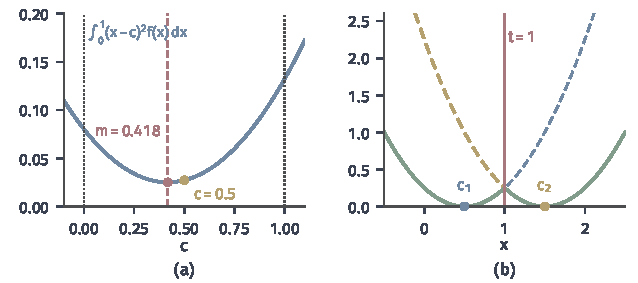
\includegraphics[width=108mm]{figures/07-probability/05-source-coding/matplotlib/quant-centroid-nn/figure.pdf}
 \caption{两个子问题的解。(a) $\operatorname{Laplace}(0,1)$在区间$[0,1)$上的平方误差$\int_0^1(x-c)^2f(x)\,\mathrm{d}x$随$c$的变化（蓝线），最低点在质心$m=0.418$（红点），区间中点$c=0.5$（黄点）处略高。(b) 固定重构值$c_1=0.5$、$c_2=1.5$时，两条虚线是$(x-c_1)^2$与$(x-c_2)^2$，绿线是它们的下包络；两者在中点$t=1$（红线）处交换。}
 \label{fig:quant-centroid-nn}
\end{BookInlineFigure}

\paragraph{固定重构值选区间}
现在反过来，重构值$c_1<\dots<c_N$固定，问每个读数应归入哪个区间。平均失真是逐点误差的期望，而逐点误差只取决于这个读数被报成哪个值。所以对每个读数分别选最近的重构值，就使平均失真最小，不需要考虑其他读数。

\begin{lemma}[最近邻条件]
\label{lem:quant-nearest}
设重构值$c_1,\dots,c_N$固定，$Q$是以它们为重构值的任一量化器。则
\begin{equation}
 D(Q)\geq\mathbb{E}\Bigl[\min_{1\leq k\leq N}(X-c_k)^{2}\Bigr] ,
 \label{eq:quant-nearest-bound}
\end{equation}
等号成立当且仅当以概率$1$有$(X-Q(X))^{2}=\min_k(X-c_k)^{2}$，即几乎每个读数都被报成离它最近的重构值。
\end{lemma}

\begin{proof}
对每个$x$，$Q(x)$是某个$c_k$，所以逐点有$(x-Q(x))^{2}\geq\min_k(x-c_k)^{2}$。两边是非负可测函数，取期望即得式~\eqref{eq:quant-nearest-bound}。两边之差是非负随机变量，它的期望为零当且仅当它几乎必然为零，这就是等号条件。
\end{proof}

最近邻规则下的区间可以直接算出来。对相邻的两个重构值，比较两种误差：
\[
 (x-c_j)^{2}-(x-c_{j+1})^{2}=(c_{j+1}-c_j)\bigl(2x-c_j-c_{j+1}\bigr) .
\]
由于$c_{j+1}>c_j$，左边小于零当且仅当$x$小于两点的中点。所以最近邻区间仍是区间，阈值是相邻重构值的中点：
\begin{equation}
 t_j=\frac{c_j+c_{j+1}}{2},\qquad j=1,\dots,N-1 .
 \label{eq:quant-midpoint-threshold}
\end{equation}
读数恰好落在中点时两个重构值一样近，需要约定归属，例如归入编号较小的一个。对有密度的读数，中点的概率为零，约定不影响平均失真。图~\ref{fig:quant-centroid-nn}右图画出两条误差抛物线和它们的下包络，交点就在中点$t=1$。

\paragraph{两条必要条件}
两个引理合起来，就是最优量化器必须满足的条件。

\begin{theorem}[Lloyd--Max条件]
\label{thm:quant-lloyd-max-conditions}
设$\mathbb{E}[X^{2}]<\infty$，平方误差下$Q^{*}$在所有$N$点量化器中平均失真最小，其区间为$S_j$、重构值为$c_j$。则：
\begin{enumerate}
 \item 对每个$p_j=\mathbb{P}(X\in S_j)>0$，$c_j=\mathbb{E}[X\mid X\in S_j]$；
 \item 以概率$1$有$(X-c_{\alpha(X)})^{2}=\min_k(X-c_k)^{2}$。
\end{enumerate}
\end{theorem}

\begin{proof}
若第一条对某个$j$不成立，由引理~\ref{lem:quant-centroid}，把$c_j$换成条件均值严格减小区间$S_j$上的误差，其余区间不变，平均失真严格下降，与$Q^{*}$最优矛盾。若第二条不成立，由引理~\ref{lem:quant-nearest}，保持重构值、按最近邻重新划分，平均失真严格下降，同样矛盾。
\end{proof}

这两条只是必要条件，不是充分条件：满足它们的量化器可能不是最优的，后面会给出例子。定理也没有断言最优量化器存在。对平方误差和二阶矩有限的读数，$N$点最优量化器确实存在：离分布太远的重构值可以拉回而不增大失真，于是只需在有界的重构值集合中寻找，再用紧性论证取到最小值。下面的迭代只用到两条必要条件，不依赖存在性。

\paragraph{交替改进的思想}
两条条件提示了一个迭代：从某组重构值出发，先按式~\eqref{eq:quant-midpoint-threshold}取中点作阈值，再按式~\eqref{eq:quant-conditional-mean}把每个重构值移到新区间的质心，然后重复。每一步都是在固定另一组变量时求得的最优解，所以平均失真不会上升。这种做法称为\term{Lloyd--Max算法}（Lloyd--Max algorithm）。写成公式，第$t$轮的两步为
\begin{equation}
 t_j^{(t)}=\frac{c_j^{(t-1)}+c_{j+1}^{(t-1)}}{2},\qquad
 c_j^{(t)}=\mathbb{E}\bigl[X\bigm| t_{j-1}^{(t)}\leq X<t_j^{(t)}\bigr] ,
 \label{eq:quant-lloyd-update}
\end{equation}
其中$t_0^{(t)}=-\infty$、$t_N^{(t)}=+\infty$。

对Laplace读数，质心有显式形式，迭代可以手算。$\operatorname{Laplace}(0,1)$在$x\geq0$上就是$\frac12\mathrm{e}^{-x}$，对$0\leq a<b$，积分得到区间的概率与条件均值：
\begin{equation}
 \begin{gathered}
 \mathbb{P}(a\leq X<b)=\frac{\mathrm{e}^{-a}-\mathrm{e}^{-b}}{2},\\
 \mathbb{E}[X\mid a\leq X<b]=\frac{(a+1)\mathrm{e}^{-a}-(b+1)\mathrm{e}^{-b}}{\mathrm{e}^{-a}-\mathrm{e}^{-b}} .
 \end{gathered}
 \label{eq:quant-laplace-centroid}
\end{equation}
令$b\to\infty$，得到$\mathbb{E}[X\mid X\geq a]=a+1$：超过$a$的部分服从$\operatorname{Exp}(1)$，均值为$1$，这是指数分布无记忆性的直接结果。负半轴由对称性得到。

\paragraph{计算过程}
下面用$N=4$、从上一小节的均匀量化器出发，逐轮演示。读数分布关于零对称，初始重构值也对称，每轮更新后仍对称，所以中间阈值始终为$0$，只需跟踪正半轴的一个阈值和两个重构值。

\needspace{6\baselineskip}
\paragraph{变量}
\begin{itemize}
 \item $c_1^{(t)}<\dots<c_N^{(t)}$：第$t$轮的重构值，共$N$个实数。
 \item $t_1^{(t)}<\dots<t_{N-1}^{(t)}$：第$t$轮的阈值，共$N-1$个实数，两端补$\pm\infty$。
 \item $D^{(t)}$：第$t$轮量化器的平均失真，用于判断何时停止。
\end{itemize}
例中由对称性，只需记录$t_3^{(t)}$、$c_3^{(t)}$与$c_4^{(t)}$。

\paragraph{初始化}
重构值初始化为一组互不相同的点，常用的选择是同样点数的均匀量化器，或者从源分布中抽取的几个值。$D^{(0)}$是这组点配上最近邻区间时的平均失真。例中取$\Delta=1$的均匀量化器，
\[
 c^{(0)}=(-1.5,\,-0.5,\,0.5,\,1.5),\qquad D^{(0)}=0.5142 .
\]

\needspace{6\baselineskip}
\paragraph{每轮更新}
在第$t$轮：
\begin{enumerate}
 \item \textbf{更新阈值。}按式~\eqref{eq:quant-lloyd-update}的第一式取相邻重构值的中点。例中第一轮
 \[
  t_3^{(1)}=\frac{0.5+1.5}{2}=1 ,
 \]
 阈值为$(-1,0,1)$，与初始量化器相同。

 \item \textbf{更新重构值。}按式~\eqref{eq:quant-lloyd-update}的第二式把每个重构值移到新区间的质心，Laplace读数用式~\eqref{eq:quant-laplace-centroid}计算。例中第一轮内侧区间是$[0,1)$，外侧是$[1,\infty)$：
 \[
  c_3^{(1)}=\frac{1-2\mathrm{e}^{-1}}{1-\mathrm{e}^{-1}}=0.4180,\qquad c_4^{(1)}=1+1=2 .
 \]
 外侧的重构值从$1.5$跳到$2$：尾部质量的重心比区间起点远一个单位。

 \item \textbf{计算平均失真。}重构值已是质心，可用式~\eqref{eq:quant-centroid-distortion}，其中$\mathbb{E}[X^2]=2$。例中两侧区间概率为$0.3161$和$0.1839$，
 \[
  D^{(1)}=2-2\bigl(0.3161\times0.4180^{2}+0.1839\times2^{2}\bigr)=0.4180 .
 \]

 \item \textbf{判断停止。}若相对下降$(D^{(t-1)}-D^{(t)})/D^{(t)}$小于预先给定的$\varepsilon$，停止；否则进入下一轮。例中取$\varepsilon=10^{-3}$，第一轮下降约$23\%$，继续。
\end{enumerate}

例中第二轮先取中点，
\[
 t_3^{(2)}=\frac{0.4180+2}{2}=1.2090 .
\]
再计算新区间的质心。由$\mathrm{e}^{-1.209}=0.2985$与式~\eqref{eq:quant-laplace-centroid}，
\[
 c_3^{(2)}=\frac{1-2.209\times0.2985}{1-0.2985}=0.4856,\qquad c_4^{(2)}=2.2090 .
\]
内侧区间概率为$(1-0.2985)/2=0.3508$，外侧为$0.1492$，于是
\[
 D^{(2)}=2-2\bigl(0.3508\times0.4856^{2}+0.1492\times2.209^{2}\bigr)=0.3781 .
\]

以后各轮照此进行。表~\ref{tab:quant-lloyd-rounds}列出前八轮的结果。阈值和外侧重构值每轮外移，内侧重构值在第一轮内移后也逐步外移，平均失真单调下降。

\begin{BookInlineTable}
 \centering
 \begin{tabular}{ccccc}
  \toprule
  $t$ & $t_3^{(t)}$ & $c_3^{(t)}$ & $c_4^{(t)}$ & $D^{(t)}$\\
  \midrule
  $0$ & $1.0000$ & $0.5000$ & $1.5000$ & $0.5142$\\
  $1$ & $1.0000$ & $0.4180$ & $2.0000$ & $0.4180$\\
  $2$ & $1.2090$ & $0.4856$ & $2.2090$ & $0.3781$\\
  $3$ & $1.3473$ & $0.5268$ & $2.3473$ & $0.3624$\\
  $4$ & $1.4370$ & $0.5521$ & $2.4370$ & $0.3563$\\
  $5$ & $1.4945$ & $0.5677$ & $2.4945$ & $0.3539$\\
  $6$ & $1.5311$ & $0.5774$ & $2.5311$ & $0.35299$\\
  $7$ & $1.5543$ & $0.5835$ & $2.5543$ & $0.35263$\\
  $8$ & $1.5689$ & $0.5873$ & $2.5689$ & $0.35248$\\
  \midrule
  $\infty$ & $1.5936$ & $0.5936$ & $2.5936$ & $0.35239$\\
  \bottomrule
 \end{tabular}
 \caption{$\operatorname{Laplace}(0,1)$、$N=4$的Lloyd--Max迭代，只列正半轴；第$0$行是初始的均匀量化器，末行是不动点。}
 \label{tab:quant-lloyd-rounds}
\end{BookInlineTable}

第七轮的相对下降为$(0.35299-0.35263)/0.35263\approx1.02\times10^{-3}$，尚未达标；第八轮为$(0.35263-0.35248)/0.35248\approx4.3\times10^{-4}$，迭代停止。最终得到的量化器为
\[
 \begin{gathered}
 t=(-1.569,\ 0,\ 1.569),\qquad D=0.3525,\\
 c=(-2.569,\ -0.587,\ 0.587,\ 2.569) .
 \end{gathered}
\]
比初始的均匀量化器的$0.5142$减少约$31\%$，点数没有变。

迭代的极限可以单独求出，用来检验上面的结果。由式~\eqref{eq:quant-laplace-centroid}，外侧质心总是$c_4=t+1$；不动点处阈值是中点，$t=(c_3+c_4)/2$，于是$c_3=t-1$。再要求$c_3$是$[0,t)$的质心，得到关于$t$的方程
\[
 t-1=\frac{1-(t+1)\mathrm{e}^{-t}}{1-\mathrm{e}^{-t}} .
\]
它的正根为$t=1.5936$，相应$c_3=0.5936$、$c_4=2.5936$，由式~\eqref{eq:quant-centroid-distortion}得$D=0.3524$。图~\ref{fig:quant-lloyd-rounds}画出迭代二十轮的轨迹，各量都向这个不动点靠拢。

\begin{BookInlineFigure}
 \centering
 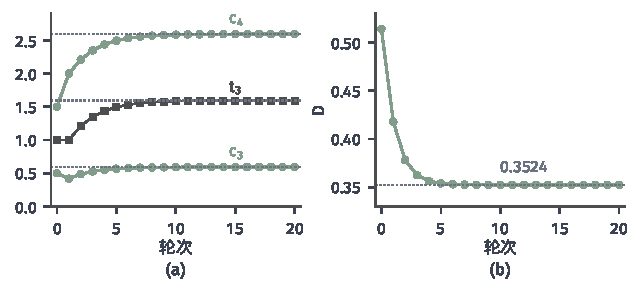
\includegraphics[width=108mm]{figures/07-probability/05-source-coding/matplotlib/quant-lloyd-rounds/figure.pdf}
 \caption{$\operatorname{Laplace}(0,1)$、$N=4$的Lloyd--Max迭代。(a) 正半轴的阈值$t_3$（灰色方块）与重构值$c_3$、$c_4$（绿色圆点）随轮次的变化，点线为不动点。(b) 平均失真随轮次单调下降，点线为不动点处的$0.3524$。}
 \label{fig:quant-lloyd-rounds}
\end{BookInlineFigure}

\paragraph{目标单调下降}
记$D(\mathcal{S},\bm{c})$为区间组$\mathcal{S}$配重构值$\bm{c}$时的平均失真。第$t$轮先由引理~\ref{lem:quant-nearest}，再由引理~\ref{lem:quant-centroid}，得到
\[
 D\bigl(\mathcal{S}^{(t)},\bm{c}^{(t)}\bigr)\leq D\bigl(\mathcal{S}^{(t)},\bm{c}^{(t-1)}\bigr)\leq D\bigl(\mathcal{S}^{(t-1)},\bm{c}^{(t-1)}\bigr) .
\]
所以$D^{(t)}$单调不增。它有下界$0$，因此收敛。

这个论证只说明平均失真的数值收敛，没有说明阈值和重构值本身收敛，更没有说明收敛到最优量化器。例中参数也收敛了，那是这个具体分布的性质。

每轮的代价是计算$N$个区间的概率与一阶矩。分布有显式的积分公式时，代价与$N$成正比；需要数值积分或模拟时，还要加上积分误差，这一点在第~\ref{sec:quant-granular-overload}节再谈。

\paragraph{初始化、空区间与并列}
初始重构值必须互不相同，否则两个点的最近邻区间无法区分。迭代中若某个区间的概率为零，它的条件均值没有定义，式~\eqref{eq:quant-lloyd-update}无法执行。对Laplace这样处处有正密度的读数，只要重构值互不相同，每个区间都有正概率，这种情况不会发生；对离散读数或支撑有空隙的读数则可能发生。常见的处理是保留原来的重构值，或者把它挪到当前误差最大的区间内，把那个区间一分为二。前一种做法仍保证目标不增，后一种改变了迭代的路线，需要重新检查单调性。

读数恰好落在两个重构值的中点时，两者一样近。对有密度的读数，这个事件概率为零；对离散读数，归属约定会改变区间的质心，从而改变后续的迭代，所以必须事先固定，例如一律归入编号较小的区间。

\paragraph{局部最优}
目标下降并不保证到达全局最小。考虑一个离散读数，等概率地取$0$、$2$、$3.5$三个值，用$N=2$个点量化。有两种不同的划分都满足Lloyd--Max条件。

第一种把$\{0\}$与$\{2,3.5\}$分开，重构值是两组的平均：
\[
 c=(0,\ 2.75),\qquad t=1.375 .
\]
$2$离$2.75$比离$0$近，划分与最近邻一致，是不动点。平均失真为
\[
 D=\frac{0+0.75^{2}+0.75^{2}}{3}=0.375 .
\]

第二种把$\{0,2\}$与$\{3.5\}$分开，
\[
 c=(1,\ 3.5),\qquad t=2.25 .
\]
$2$离$1$的距离是$1$，离$3.5$是$1.5$，仍归第一组，也是不动点。平均失真为
\[
 D=\frac{1+1+0}{3}=0.667 .
\]

从$c^{(0)}=(0,1)$出发，阈值$0.5$给出第一种划分；从$c^{(0)}=(1,4)$出发，阈值$2.5$给出第二种划分。两次迭代都在第一轮后停住，结果相差近一倍。图~\ref{fig:quant-lloyd-local}画出这两个不动点。

\begin{BookInlineFigure}
 \centering
 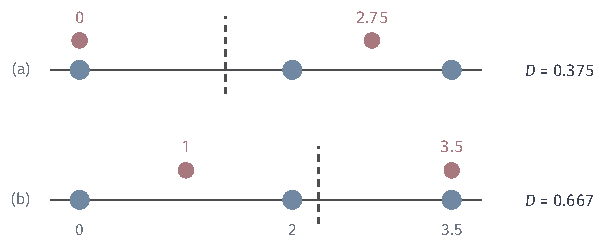
\includegraphics[width=102.5mm]{figures/07-probability/05-source-coding/tikz/quant-lloyd-local/figure.pdf}
 \caption{等概率取$0$、$2$、$3.5$（蓝点）的读数用两个点量化时的两个Lloyd--Max不动点。红点为重构值，虚线为阈值。(a) 划分$\{0\}$、$\{2,3.5\}$，$D=0.375$，是全局最优；(b) 划分$\{0,2\}$、$\{3.5\}$，$D=0.667$，也满足两条必要条件，但不是最优。}
 \label{fig:quant-lloyd-local}
\end{BookInlineFigure}

所以实际计算中常从多组初始值出发，保留平均失真最小的结果。对一维有密度的读数，若密度的对数是凹函数（Laplace与高斯都满足），满足两条条件的量化器只有一个，Lloyd--Max迭代因而收敛到全局最优。证明要说明不动点方程组只有一个解，需要逐个比较阈值的单调性，篇幅较长；上面Laplace例子的不动点方程只有一个正根，与这一结论相符。

\paragraph{与均匀量化的比较}
同样的迭代可以用于任意点数。图~\ref{fig:quant-lloydmax-vs-uniform}比较$N=8$时Lloyd--Max的不动点与最好的均匀量化器（步长在所有$\Delta$中搜索得到）。Lloyd--Max的区间在中央最窄、向外逐渐变宽，最外侧的重构值远达$\pm4.37$；均匀量化器的步长约为$1.03$，范围只到$\pm4.13$。两者的平均失真分别为$0.1090$与$0.1435$，在同样$3$个比特下，按分布调整的划分把误差降低了约$24\%$。

\begin{BookInlineFigure}
 \centering
 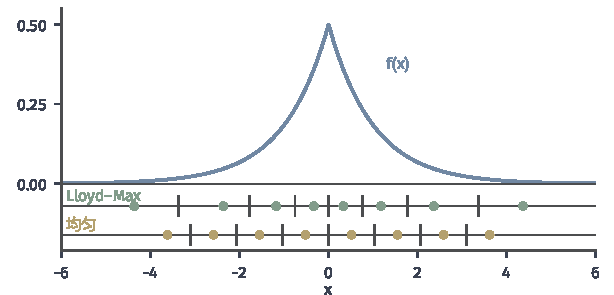
\includegraphics[width=104mm]{figures/07-probability/05-source-coding/matplotlib/quant-lloydmax-vs-uniform/figure.pdf}
 \caption{$\operatorname{Laplace}(0,1)$的两个8点量化器。蓝线为密度。上一行绿点为Lloyd--Max不动点的重构值，竖线为阈值；下一行黄点为最好的均匀量化器的重构值（步长约$1.03$）。Lloyd--Max在中央划得更细、在尾部划得更粗。}
 \label{fig:quant-lloydmax-vs-uniform}
\end{BookInlineFigure}

代价在实现上。均匀量化的编码器按式~\eqref{eq:quant-uniform-encoder}一次除法和取整就能完成，非均匀量化则要把读数与$N-1$个阈值比较（二分查找需要约$\log_2N$次比较），并且需要知道源分布才能设计。


\section{向量量化}
\label{sec:quant-vector}

传感器常常连续读数，相邻两次读数彼此接近。若把每个读数单独量化，量化器看不到这种联系。把两个读数合成一个二维向量，再整体选择重构点，能否在相同的每分量比特数下做得更好？这一节说明答案是肯定的，并说明好处来自哪里、代价在哪里。

\paragraph{逐分量码本与联合码本}
对$d$维读数$\bm{X}=(X_1,\dots,X_d)$，最直接的做法是给每个分量配一个标量量化器，各分量独立编码。若第$i$个分量用$N_i$个点，合起来的重构点是各分量重构值的全部组合，共$N=N_1\cdots N_d$个，区域是坐标轴方向的长方体。这样的量化器称为\term{乘积量化器}（product quantizer），它的码本称为逐分量码本。

更一般的做法是直接在$\mathbb{R}^{d}$中选$N$个点$\bm{c}_1,\dots,\bm{c}_N$作为码本，区域不必是长方体。这就是第~\ref{sec:quant-model}节定义中的$d$维量化器，称为\term{向量量化}（vector quantization），它的码本称为联合码本。乘积量化器是它的特例，所以在相同点数下，最好的联合码本不会比最好的逐分量码本差。按式~\eqref{eq:quant-rate-per-component}，两者每分量的比特数都是$\frac1d\log_2N$。

\paragraph{两条条件的推广}
平方误差取$\lVert\bm{x}-\hat{\bm{x}}\rVert_2^{2}$。第~\ref{sec:quant-nonuniform}节的两个引理在$d$维中照样成立，证明只需把乘积换成内积。

对质心条件，设区域$S$的概率$p>0$，条件均值$\bm{m}=\mathbb{E}[\bm{X}\mid\bm{X}\in S]$。展开平方范数，
\[
 \lVert\bm{X}-\bm{c}\rVert_2^{2}=\lVert\bm{X}-\bm{m}\rVert_2^{2}+2\langle\bm{X}-\bm{m},\bm{m}-\bm{c}\rangle+\lVert\bm{m}-\bm{c}\rVert_2^{2} .
\]
交叉项乘$\mathbf{1}_{\{\bm{X}\in S\}}$后期望为零，于是
\begin{equation}
 \mathbb{E}\bigl[\lVert\bm{X}-\bm{c}\rVert_2^{2}\mathbf{1}_{\{\bm{X}\in S\}}\bigr]=\mathbb{E}\bigl[\lVert\bm{X}-\bm{m}\rVert_2^{2}\mathbf{1}_{\{\bm{X}\in S\}}\bigr]+p\lVert\bm{m}-\bm{c}\rVert_2^{2} ,
 \label{eq:quant-vector-parallel-axis}
\end{equation}
最好的重构点仍是区域的质心。最近邻条件的证明与维数无关，逐点取最近的重构点即可。

最近邻规则下的区域有明确的几何形状。$\bm{x}$离$\bm{c}_j$不比离$\bm{c}_k$远，即
\[
 \lVert\bm{x}-\bm{c}_j\rVert_2^{2}\leq\lVert\bm{x}-\bm{c}_k\rVert_2^{2} .
\]
展开两边，$\lVert\bm{x}\rVert_2^{2}$相消，条件化为
\[
 2\langle\bm{x},\bm{c}_k-\bm{c}_j\rangle\leq\lVert\bm{c}_k\rVert_2^{2}-\lVert\bm{c}_j\rVert_2^{2} .
\]
这是以$\bm{c}_j$与$\bm{c}_k$连线的垂直平分面为边界的半空间。对所有$k\neq j$取交集，得到
\begin{equation}
 V_j=\bigl\{\bm{x}\in\mathbb{R}^{d}:\ \lVert\bm{x}-\bm{c}_j\rVert_2\leq\lVert\bm{x}-\bm{c}_k\rVert_2,\ k=1,\dots,N\bigr\} ,
 \label{eq:quant-voronoi}
\end{equation}
称为$\bm{c}_j$的\term{Voronoi区域}（Voronoi region）。它是有限个半空间的交，因而是凸多面体（可以无界）。各$V_j$只在边界上重叠，边界属于哪一个仍按编号约定；一维时它们就是以中点为端点的区间。

\paragraph{广义Lloyd算法}
于是标量的交替改进可以原样搬过来：固定码本，按式~\eqref{eq:quant-voronoi}把读数分给最近的码字；固定区域，把每个码字移到区域的质心。第~\ref{sec:quant-nonuniform}节的单调性论证逐字适用，平均失真单调不增。这一推广称为\term{广义Lloyd算法}（generalized Lloyd algorithm）。

二维以上的区域是多边形或多面体，质心一般没有显式公式。实际计算时，常用从源分布模拟出的大量向量的平均代替期望：区域的质心换成落在区域中的模拟向量的平均，平均失真换成模拟向量的平均误差。这样得到的是对期望的近似，其误差由第~\ref{chap:monte-carlo-integration-error}章的方法估计；若这些向量不是模拟出来的，而是观测到的数据，从数据估计量化器就属于统计推断的问题，由卷八处理。

\paragraph{相关结构的利用}
先看一个可以手算的例子。读数$\bm{X}=(X_1,X_2)$在两个单位正方形的并集
\[
 A=[0,1]^{2}\cup[1,2]^{2}
\]
上均匀分布，两个正方形各占概率$\tfrac12$。两个分量高度相关：$X_1$小时$X_2$也小。每个分量允许1 bit，即$N=4$。

先用逐分量码本。$X_1$的分布是$[0,1]$与$[1,2]$上各一半的均匀分布，合起来是$[0,2]$上的均匀分布，$X_2$也一样。每个分量最好的两点量化器取区间中点$0.5$与$1.5$，每分量误差为
\[
 \mathbb{E}\bigl[(X_1-Q_1(X_1))^{2}\bigr]=\frac{1^{2}}{12}=\frac{1}{12},
\]
每个向量的平方误差为$\tfrac16$。四个组合点中，$(0.5,1.5)$与$(1.5,0.5)$落在两个空白方块里，它们的区域概率为零，从不被使用。图~\ref{fig:quant-two-squares}左图画出了这种浪费。

\begin{BookInlineFigure}
 \centering
 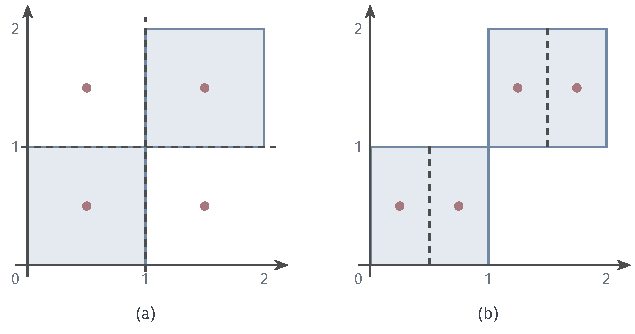
\includegraphics[width=107.5mm]{figures/07-probability/05-source-coding/tikz/quant-two-squares/figure.pdf}
 \caption{在两个单位正方形（浅蓝）上均匀分布的二维读数，用4个点量化。(a) 逐分量码本：每个分量取$0.5$与$1.5$，红点是全部4个组合，虚线是区域边界；两个点落在空白处，从不使用，每个向量的平方误差为$1/6$。(b) 联合码本：每个正方形沿竖直中线一分为二，各放一个质心，平方误差为$5/48$。}
 \label{fig:quant-two-squares}
\end{BookInlineFigure}

若对这个逐分量码本运行广义Lloyd算法，第一轮最近邻分配就会使两个空白方块中的码字分不到任何读数，出现第~\ref{sec:quant-nonuniform}节所说的空区域。按“挪到误差最大的区域并一分为二”的处理，每个被使用的码字区域分出一半给空闲码字，得到右图的联合码本：
\[
 (0.25,0.5),\quad(0.75,0.5),\quad(1.25,1.5),\quad(1.75,1.5) .
\]
每个区域是$\tfrac12\times1$的长方形，读数在其中均匀分布。由式~\eqref{eq:quant-vector-parallel-axis}，以质心为重构点时，误差就是两个坐标方向的方差之和，
\[
 \frac{(1/2)^{2}}{12}+\frac{1^{2}}{12}=\frac{1}{48}+\frac{4}{48}=\frac{5}{48} .
\]
这组码本满足两条条件：每个码字是区域质心，区域也正是最近邻区域。联合码本把每个向量的平方误差从$\tfrac{8}{48}$降到$\tfrac{5}{48}$，减少$37.5\%$，而每分量仍是1 bit。好处来自把四个点全部放在读数真正出现的地方。

图~\ref{fig:quant-gauss-vq}对连续分布做同样的比较。读数是相关系数$0.9$、方差为$1$的二维高斯向量，$N=16$，每分量2 bit。左图是两个4点Lloyd--Max标量量化器的乘积，每分量误差是标量值$0.1175$。十六个长方形中只有十个的概率超过千分之一，其余几乎不用。右图是从左图码本出发、在$2\times10^{5}$个模拟向量上运行广义Lloyd算法得到的联合码本：码字沿对角线排成一串，区域是与对角线垂直的长条。在另外$2\times10^{5}$个独立模拟向量上计算，每分量误差约为$0.0442$，不到逐分量码本的四成。

\begin{BookInlineFigure}
 \centering
 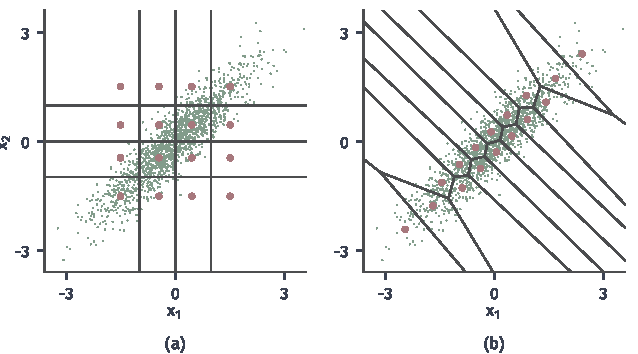
\includegraphics[width=108mm]{figures/07-probability/05-source-coding/matplotlib/quant-gauss-vq/figure.pdf}
 \caption{相关系数$0.9$的二维标准高斯读数，16个码字。绿点为1500个模拟读数，红点为码字，灰线为区域边界。(a) 逐分量4点Lloyd--Max码本，每分量误差$0.1175$。(b) 广义Lloyd算法得到的联合码本（$2\times10^{5}$个训练向量，种子1），区域为Voronoi区域；在独立的$2\times10^{5}$个向量（种子2）上每分量误差约为$0.0442$。}
 \label{fig:quant-gauss-vq}
\end{BookInlineFigure}

\paragraph{区域形状的利用}
即使分量相互独立，联合码本仍有一点好处，来自区域的形状。设读数在一个区域内近似均匀分布，区域面积为$V$，重构点在区域的质心。为了比较形状而不受大小影响，把每分量的平方误差除以$V^{2/d}$，得到无量纲的\term{归一化二阶矩}（normalized second moment）
\begin{equation}
 G=\frac{1}{d}\,\frac{1}{V^{1+2/d}}\int_{\text{区域}}\lVert\bm{x}-\bm{c}\rVert_2^{2}\,\mathrm{d}\bm{x} ,
 \label{eq:quant-normalized-moment}
\end{equation}
$G$越小，同样面积的区域给出的误差越小。逐分量量化在独立同分布的分量上产生正方形区域，联合码本可以用其他形状铺满平面。

单位正方形以中心为重构点时，两个方向各贡献$\tfrac1{12}$，所以$G=\tfrac1{12}\approx0.0833$。正六边形可以用平行轴恒等式~\eqref{eq:quant-vector-parallel-axis}计算。把边长为$a$的正六边形分成六个边长为$a$的正三角形，每个三角形的面积为$A_{\triangle}=\frac{\sqrt3}{4}a^{2}$，直接积分可得它绕自身质心的二阶矩是$A_{\triangle}a^{2}/12$。三角形的质心离六边形中心$a/\sqrt3$，由式~\eqref{eq:quant-vector-parallel-axis}，绕六边形中心的二阶矩为
\[
 A_{\triangle}\Bigl(\frac{a^{2}}{12}+\frac{a^{2}}{3}\Bigr)=\frac{5}{12}A_{\triangle}a^{2} .
\]
六个三角形合起来，面积为$6A_{\triangle}$，二阶矩为$6\cdot\frac{5}{12}A_{\triangle}a^{2}$。取面积为$1$，即$a^{2}=\frac{2}{3\sqrt3}$，代入式~\eqref{eq:quant-normalized-moment}，
\[
 G=\frac12\cdot\frac{5}{12}a^{2}=\frac{5}{36\sqrt3}\approx0.0802 .
\]

\begin{BookInlineFigure}
 \centering
 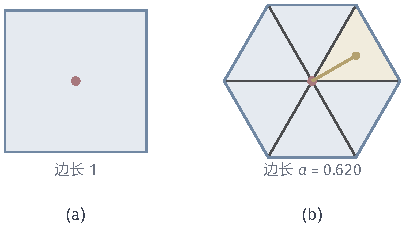
\includegraphics[width=68.6mm]{figures/07-probability/05-source-coding/tikz/quant-cell-shapes/figure.pdf}
 \caption{面积同为$1$的两种区域，红点为重构点。(a) 正方形，$G=1/12\approx0.0833$。(b) 正六边形分成六个正三角形；黄色三角形的质心（黄点）离中心$a/\sqrt3$，由平行轴恒等式求得$G=5/(36\sqrt3)\approx0.0802$。}
 \label{fig:quant-cell-shapes}
\end{BookInlineFigure}

图~\ref{fig:quant-cell-shapes}比较了这两种形状。六边形比正方形更接近圆，离重构点远的角少，在相同面积下误差约小$3.8\%$。这个收益只在区域很多、边界效应可以忽略时才显现，而且只有联合码本才能取得，因为逐分量量化的区域永远是长方体。与相关结构带来的收益相比，形状收益不大；但它说明即使分量独立，逐个读数量化也不是最好的做法。

\paragraph{存储、搜索与局部最优的代价}
联合码本的收益需要付出代价。固定每分量$R$个比特，码字个数为
\begin{equation}
 N=2^{dR} ,
 \label{eq:quant-codebook-size}
\end{equation}
随维数$d$指数增长。表~\ref{tab:quant-vq-cost}列出几种情形：存储码本需要$Nd$个实数，对每个读数做穷举最近邻搜索需要计算$N$个距离，约$Nd$次乘法。逐分量码本只需存储$d$个标量量化器，共$d2^{R}$个数，编码时各分量独立查找。

\begin{BookInlineTable}
 \centering
 \begin{tabular}{rrrrr}
  \toprule
  $d$ & $R$ & $N=2^{dR}$ & 联合码本存储$Nd$ & 逐分量存储$d2^{R}$\\
  \midrule
  $2$ & $2$ & $16$ & $32$ & $8$\\
  $4$ & $2$ & $256$ & $1024$ & $16$\\
  $8$ & $2$ & $65536$ & $524288$ & $32$\\
  $16$ & $1$ & $65536$ & $1048576$ & $32$\\
  \bottomrule
 \end{tabular}
 \caption{每分量$R$ bit时联合码本与逐分量码本的规模。穷举搜索每个读数的乘法次数与联合码本存储量同阶。}
 \label{tab:quant-vq-cost}
\end{BookInlineTable}

设计码本也更困难。广义Lloyd算法每轮要对每个模拟向量计算$N$个距离，而且目标函数有许多局部最小值，结果依赖初值。图~\ref{fig:quant-vq-inits}在前面的相关高斯例子上，从十组随机初值出发各迭代四十轮：所有轨迹都降到逐分量码本的误差之下，最终的每分量误差分布在$0.0439$到$0.0455$之间，彼此相差约$4\%$。维数和码字更多时，这种差异通常更大。

\begin{BookInlineFigure}
 \centering
 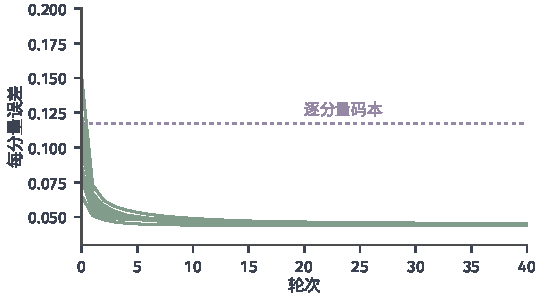
\includegraphics[width=92mm]{figures/07-probability/05-source-coding/matplotlib/quant-vq-inits/figure.pdf}
 \caption{相关系数$0.9$的二维高斯读数、16个码字时，广义Lloyd算法从十组初值出发的每分量误差（绿线，在$5\times10^{4}$个模拟向量上计算，种子1；初值为随机抽取的16个模拟向量，种子11至20）。紫色点线为逐分量4点Lloyd--Max码本的误差$0.1175$。各轨迹单调下降，但停在不同的值上。}
 \label{fig:quant-vq-inits}
\end{BookInlineFigure}

所以向量量化的维数是一种权衡：维数越高，越能利用相关结构和区域形状，码本存储、搜索和设计的代价也越高。实际系统常用有结构的码本（例如由格点构成的码本，或分级、分组的码本）来降低搜索代价，代价是放弃一部分失真上的收益。


\section{量化索引的压缩}
\label{sec:quant-index-coding}

到目前为止，每个索引都按定长写出，$N$个点用$\log_2N$个比特。可是索引并不等可能：Laplace读数的四点Lloyd--Max量化器中，内侧两个区间各占约$40\%$，外侧两个各占约$10\%$。上一章说过，概率不均匀的离散信源可以用变长码缩短平均长度。量化索引正是这样一个离散信源。

\paragraph{固定量化器后的索引编码}
量化器固定后，索引$J=\alpha(X)$的分布由式~\eqref{eq:quant-index-pmf}给出。对$J$使用第~\ref{chap:lossless-coding}章的前缀码，接收端能精确恢复$J$，再由解码器报出同一个重构值。重构结果、从而平均失真都没有改变，改变的只是平均描述长度。由上一章的平均码长界，最好的前缀码满足
\begin{equation}
 H(J)\leq\bar{\ell}<H(J)+1 ,
 \label{eq:quant-index-length-bound}
\end{equation}
其中$\bar{\ell}=\sum_jp_j\ell(j)$是平均码长，$H(J)$是索引的熵。

以第~\ref{sec:quant-nonuniform}节得到的四点不动点量化器为例。外侧区间$\lvert X\rvert\geq1.5936$的概率是$\mathrm{e}^{-1.5936}=0.2032$，两侧平分，于是索引的分布为
\[
 (p_1,p_2,p_3,p_4)=(0.1016,\ 0.3984,\ 0.3984,\ 0.1016) .
\]
它的熵为
\[
 H(J)=-2\bigl(0.1016\log_20.1016+0.3984\log_20.3984\bigr)=1.728\ \text{bit} .
\]

用Huffman编码构造码树：先合并两个最小的概率$0.1016$与$0.1016$，得$0.2032$；再与一个$0.3984$合并，得$0.6016$；最后与另一个$0.3984$合并。码长依次为$1,2,3,3$，平均码长为
\[
 \bar{\ell}=0.3984\times1+0.3984\times2+0.1016\times3\times2=1.805\ \text{bit} .
\]
图~\ref{fig:quant-index-huffman}画出了这棵码树。与定长的$2$个比特相比，平均每个读数省下约$0.2$个比特，平均失真仍是$0.3524$。若把两个读数的索引组成一对再编码，每读数的平均码长不超过$H(J)+\tfrac12$；块越长，越接近$1.728$。

\begin{BookInlineFigure}
 \centering
 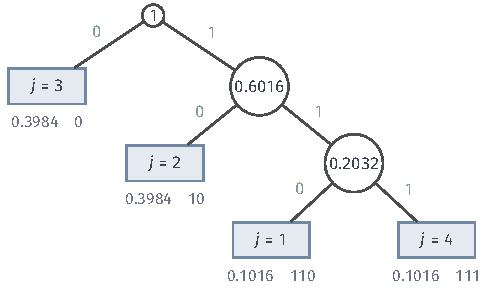
\includegraphics[width=83.4mm]{figures/07-probability/05-source-coding/tikz/quant-index-huffman/figure.pdf}
 \caption{$\operatorname{Laplace}(0,1)$四点Lloyd--Max量化器索引的Huffman码树。叶结点下方是区间概率与码字，内部结点标出合并后的概率，绿色数字是分支标号。平均码长为$1.805$ bit，索引的熵为$1.728$ bit。}
 \label{fig:quant-index-huffman}
\end{BookInlineFigure}

\paragraph{均匀量化配合熵编码}
变长描述还改变了对有限范围的要求。定长索引必须事先限定点数，因而必须规定表示范围，范围外的读数产生过载误差。变长描述却可以使用无穷多个区间：取步长为$\Delta$、零为重构值的均匀刻度，
\begin{equation}
 Q_{\Delta}(x)=\Delta\Bigl\lfloor\frac{x}{\Delta}+\frac12\Bigr\rfloor ,
 \label{eq:quant-midtread}
\end{equation}
它把$[(k-\frac12)\Delta,(k+\frac12)\Delta)$映到$k\Delta$，$k$取遍全体整数。远处的区间概率极小，给它们很长的码字，对平均长度几乎没有影响，而误差始终不超过$\Delta/2$。

索引集合可数无穷时，Huffman编码的构造不再直接适用，但长度为$\ell(k)=\lceil-\log_2p_k\rceil$的前缀码仍然存在：这些长度满足$\sum_k2^{-\ell(k)}\leq\sum_kp_k=1$，按长度从短到长依次在码树上分配码字即可，平均长度小于$H(J)+1$。所以对均匀量化配合熵编码，描述资源由索引的熵衡量。

\paragraph{索引熵与微分熵}
步长很小时，索引的熵可以用读数的微分熵近似。回顾第~\ref{chap:information-measures}章，具有密度$f$的读数的微分熵是
\[
 h(X)=-\int f(x)\log_2f(x)\,\mathrm{d}x .
\]
对Laplace读数，$-\log_2f(x)=1+\lvert x\rvert\log_2\mathrm{e}$，又$\mathbb{E}\lvert X\rvert=1$，所以
\[
 h(X)=1+\log_2\mathrm{e}=\log_2(2\mathrm{e})\approx2.443\ \text{bit} .
\]

若密度在每个长度为$\Delta$的区间内变化不大，区间概率近似为$p_k\approx f(k\Delta)\Delta$。代入索引的熵，
\[
 H(J)=-\sum_kp_k\log_2p_k\approx-\sum_kp_k\log_2f(k\Delta)-\log_2\Delta .
\]
第一项是$-\log_2f$在区间代表点上按区间概率加权的和，在$\Delta\to0$时趋于积分$h(X)$。于是
\begin{equation}
 H\bigl(Q_{\Delta}(X)\bigr)\approx h(X)-\log_2\Delta .
 \label{eq:quant-index-entropy-highres}
\end{equation}
步长减半，索引的熵增加一个比特，相当于每个区间分成两半、需要多问一个是非题。在密度足够规则（例如Riemann可积且$H(Q_1(X))$有限）时，式~\eqref{eq:quant-index-entropy-highres}两边之差在$\Delta\to0$时趋于零，证明可查阅~\scite{math-cover2006information}。

\begin{BookInlineFigure}
 \centering
 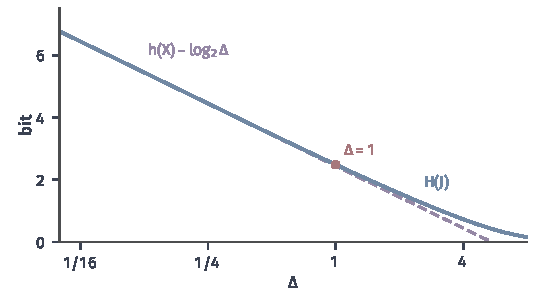
\includegraphics[width=92mm]{figures/07-probability/05-source-coding/matplotlib/quant-entropy-step/figure.pdf}
 \caption{$\operatorname{Laplace}(0,1)$读数经步长为$\Delta$的无穷均匀量化器~\eqref{eq:quant-midtread}后索引的熵。蓝线为精确值，紫色虚线为近似$h(X)-\log_2\Delta$，$h(X)=\log_2(2\mathrm{e})$；横轴为对数刻度。红点为$\Delta=1$，精确值$2.484$ bit，近似值$2.443$ bit。}
 \label{fig:quant-index-entropy}
\end{BookInlineFigure}

图~\ref{fig:quant-index-entropy}比较两者。$\Delta=1$时精确值为$2.484$ bit，近似值为$2.443$ bit，已经相当接近；步长再小，两条曲线几乎重合。步长大到与分布的尺度相当时近似失效：$\Delta=4$时近似值为负，而熵不可能为负，此时中央区间的概率已达$0.865$。

\paragraph{比较时固定相同的资源}
现在可以在相同的平均描述长度下比较不同方案。图~\ref{fig:quant-operational}画出Laplace读数的平均失真随每读数比特数的变化。黄线和绿线是定长索引的最好均匀量化器与Lloyd--Max量化器，横坐标为$\log_2N$；蓝线是无穷均匀量化器配合熵编码，横坐标为索引的熵$H(J)$；红点是四点Lloyd--Max量化器配合熵编码。

\begin{BookInlineFigure}
 \centering
 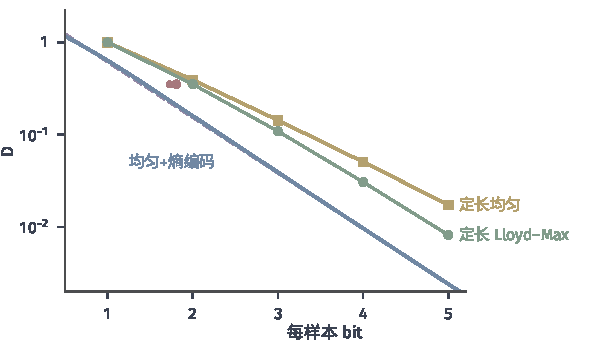
\includegraphics[width=100mm]{figures/07-probability/05-source-coding/matplotlib/quant-operational/figure.pdf}
 \caption{$\operatorname{Laplace}(0,1)$读数的平均失真与每读数比特数（纵轴为对数刻度）。黄色方块：定长索引的最好均匀量化器，$N=2,4,\dots,32$；绿色圆点：定长索引的Lloyd--Max量化器；蓝线：无穷均匀量化器配合熵编码，横坐标为索引的熵；紫色虚线：高分辨率公式$\frac{(2\mathrm{e})^{2}}{12}2^{-2R}$，与蓝线几乎重合；红点：四点Lloyd--Max量化器配合Huffman码（$1.805$ bit）与理想码长（$1.728$ bit）。}
 \label{fig:quant-operational}
\end{BookInlineFigure}

图中的排序很清楚。在约$1.8$ bit处，四点Lloyd--Max量化器加Huffman码的失真是$0.352$，而步长约为$1.66$的均匀量化器加熵编码，失真只有$0.212$。在定长$3$ bit处，Lloyd--Max量化器的失真是$0.109$；均匀量化器加熵编码只用约$2.5$ bit（$\Delta=1$）就达到$0.081$。分布越不均匀、尾部越重，这种差距越明显。

蓝线在比特数较大时几乎是一条直线，斜率对应“每多一个比特，失真降为四分之一”。这可以由两个近似合起来解释：范围内的误差近似为$\Delta^{2}/12$（第~\ref{sec:quant-granular-overload}节），索引熵近似为式~\eqref{eq:quant-index-entropy-highres}。消去$\Delta$，得到平均描述长度为$R$时
\begin{equation}
 D\approx\frac{1}{12}\,2^{2h(X)}\,2^{-2R} .
 \label{eq:quant-highres-ec}
\end{equation}
这是一个高分辨率近似，紫色虚线就是它；在$R$较小时它不再可靠。

\paragraph{把码长写进目标}
上面的方案先设计量化器、再压缩索引，两步是分开的。若平均码长才是真正的预算，那么区间和重构值也应当按这个预算来设计，而不是按点数来设计。这时“固定点数$N$”不再代表固定的描述资源：一个有许多点、但大部分点概率很小的量化器，平均码长可以很短。

把平均码长写进目标，对给定的乘子$\lambda>0$，最小化
\begin{equation}
 J_{\lambda}=D+\lambda\bar{\ell}=\mathbb{E}\bigl[(X-c_{\alpha(X)})^{2}\bigr]+\lambda\,\mathbb{E}\bigl[\ell(\alpha(X))\bigr] .
 \label{eq:quant-ecsq-objective}
\end{equation}
$\lambda$表示一个比特值多少平方误差：$\lambda$大，就更看重短码。改变$\lambda$得到不同的失真与码长组合。这样设计的量化器称为\term{熵约束量化}（entropy-constrained quantization）。

式~\eqref{eq:quant-ecsq-objective}仍是逐点代价的期望，读数$x$归入区间$j$的代价是$(x-c_j)^{2}+\lambda\ell(j)$。所以最近邻条件要修改为：把读数分给使这个带罚代价最小的$j$。比较相邻的两个重构值$c_j<c_{j+1}$，读数归入$j$当且仅当
\[
 (x-c_j)^{2}+\lambda\ell(j)\leq(x-c_{j+1})^{2}+\lambda\ell(j+1) .
\]
展开后，与第~\ref{sec:quant-nonuniform}节的计算相同，阈值从中点移到
\begin{equation}
 t_j=\frac{c_j+c_{j+1}}{2}+\frac{\lambda\bigl(\ell(j+1)-\ell(j)\bigr)}{2(c_{j+1}-c_j)} .
 \label{eq:quant-ecsq-threshold}
\end{equation}
码长较长的那个重构值，区间被压缩；读数要离它足够近，节省的误差才抵得上多付的码长。

以四点Lloyd--Max量化器为起点，取理想码长$\ell(j)=-\log_2p_j$，即内侧$1.328$ bit、外侧$3.299$ bit，以及$\lambda=0.5$。由式~\eqref{eq:quant-ecsq-threshold}，正半轴的阈值从$1.5936$移到
\[
 t_3=1.5936+\frac{0.5\times(3.299-1.328)}{2\times2}=1.840 .
\]
图~\ref{fig:quant-ecsq-threshold}画出了带罚代价的两条抛物线和移动后的交点。

\begin{BookInlineFigure}
 \centering
 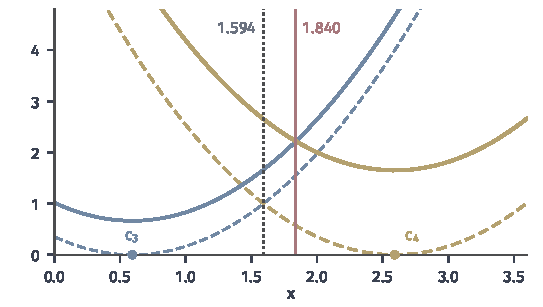
\includegraphics[width=92mm]{figures/07-probability/05-source-coding/matplotlib/quant-ecsq-threshold/figure.pdf}
 \caption{熵约束下的阈值。蓝色与黄色分别对应内侧重构值$c_3=0.594$（码长$1.328$ bit）与外侧重构值$c_4=2.594$（码长$3.299$ bit）。虚线为$(x-c_j)^{2}$，交于中点$1.594$；实线为$(x-c_j)^{2}+\lambda\ell(j)$，$\lambda=0.5$，交点右移到$1.840$（红线）。}
 \label{fig:quant-ecsq-threshold}
\end{BookInlineFigure}

阈值确定后，接着做两件事：把重构值移到新区间的质心，再把码长更新为新区间概率的理想码长。例中外侧区间概率降为$\mathrm{e}^{-1.840}/2=0.0794$，内侧升为$0.4206$；由式~\eqref{eq:quant-laplace-centroid}，新的质心为
\[
 c_3=0.6526,\qquad c_4=2.8400 .
\]
新的码长为$1.250$ bit与$3.655$ bit。平均失真升到$0.3608$，平均码长降到$1.631$ bit，目标$J_{0.5}$从$0.3524+0.5\times1.728=1.2165$降到$1.1765$。

这三步各自不增加$J_{\lambda}$。分配一步是对每个读数取带罚代价最小的区间，质心一步只改变失真项，理由与第~\ref{sec:quant-nonuniform}节相同。码长一步固定区间概率$p_j$，在$\sum_j2^{-\ell(j)}\leq1$下最小化$\sum_jp_j\ell(j)$；允许非整数码长时，上一章用KL散度的非负性证明了最小值在$\ell(j)=-\log_2p_j$取到，等于$H(J)$。实际码长必须是整数，理想码长只是这一步的近似，实际平均码长比它多不到一个比特，用块编码可以把这部分摊薄。

$\lambda$越大，外侧区间越被压缩，最终某些区间的概率可能趋于零，相当于自动减少了点数。在高分辨率下，可以说明熵约束量化的最优解接近均匀刻度，这与图~\ref{fig:quant-operational}中均匀量化加熵编码表现最好是一致的。总之，固定点数与固定平均码率是两种不同的约束，以平均码长为预算时，必须把它写进设计目标。


\section{量化误差}
\label{sec:quant-error}

前几节只用平均失真一个数评价量化器。误差本身是一个随机变量，记为
\[
 E=Q(X)-X .
\]
关于它还可以问三个问题：典型的大小是多少，偶尔会大到什么程度，它与读数之间有什么关系。第一个问题决定平均失真，第二个问题关系到最坏情形，第三个问题关系到能否把量化看成“读数加上一点独立噪声”。这一节对已经构造的量化器回答这三个问题，并说明加入共享的随机扰动怎样改变第三个问题的答案。

\subsection{舍入误差与过载误差}
\label{sec:quant-granular-overload}

考虑第~\ref{sec:quant-uniform}节的均匀量化器：$N$个点、步长$\Delta$、范围$[-L,L]$，$L=N\Delta/2$，范围外饱和。按读数是否落在范围内，把平均失真分成两部分：
\begin{equation}
 D=\underbrace{\mathbb{E}\bigl[E^{2}\mathbf{1}_{\{\lvert X\rvert\leq L\}}\bigr]}_{D_{\mathrm{gran}}}+\underbrace{\mathbb{E}\bigl[E^{2}\mathbf{1}_{\{\lvert X\rvert>L\}}\bigr]}_{D_{\mathrm{over}}} .
 \label{eq:quant-granular-overload}
\end{equation}
第一部分是舍入误差的贡献，第二部分是过载误差的贡献。

\paragraph{误差随读数的变化}
图~\ref{fig:quant-error-shape}左图画出$N=8$、$\Delta=1$时误差随读数的变化。范围内误差是锯齿形，在每个区间内从$+\tfrac12$线性降到$-\tfrac12$；范围外误差随读数线性增长，没有上界。

\begin{BookInlineFigure}
 \centering
 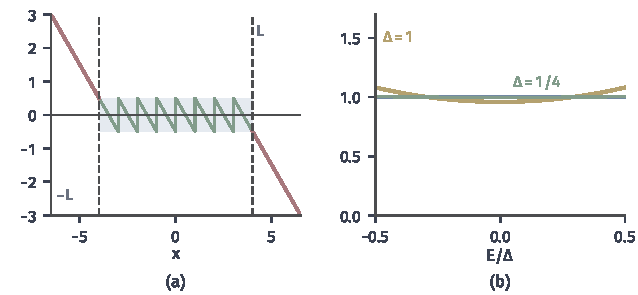
\includegraphics[width=108mm]{figures/07-probability/05-source-coding/matplotlib/quant-error-shape/figure.pdf}
 \caption{均匀量化的误差。(a) $N=8$、$\Delta=1$时$E=Q(x)-x$随读数的变化：范围内（浅蓝带，$\lvert E\rvert\leq\frac12$）为绿色锯齿，范围外为红色直线。(b) 对$\operatorname{Laplace}(0,1)$读数，在不过载的条件下$E/\Delta$的精确密度：黄线为$\Delta=1$（$N=8$），绿线为$\Delta=1/4$（$N=32$），两者范围同为$[-4,4]$；蓝线为均匀密度$1$。}
 \label{fig:quant-error-shape}
\end{BookInlineFigure}

\paragraph{舍入误差}
范围内的读数与所在区间的中点相距不超过$\Delta/2$，所以总有
\[
 D_{\mathrm{gran}}\leq\frac{\Delta^{2}}{4}\,\mathbb{P}\bigl(\lvert X\rvert\leq L\bigr) .
\]
这个界对任何分布都成立，但通常偏大四倍左右。

更常用的是一个近似。若密度在每个区间内几乎不变，那么在读数落在某个区间的条件下，它近似均匀分布于这个区间，误差近似均匀分布于$[-\Delta/2,\Delta/2]$。对均匀分布直接积分，
\[
 \frac{1}{\Delta}\int_{-\Delta/2}^{\Delta/2}e^{2}\,\mathrm{d}e=\frac{\Delta^{2}}{12} .
\]
把各区间合起来，得到
\begin{equation}
 D_{\mathrm{gran}}\approx\frac{\Delta^{2}}{12}\,\mathbb{P}\bigl(\lvert X\rvert\leq L\bigr) .
 \label{eq:quant-granular-approx}
\end{equation}
这称为\term{高分辨率近似}（high-resolution approximation）。它不是精确公式：条件是密度在区间尺度上变化很小，$\Delta$越小越准确。

近似的偏差可以用质心条件看清楚。由引理~\ref{lem:quant-centroid}，一个区间内以中点$c_j$为重构值的条件平方误差，等于条件方差加上质心与中点距离的平方。以Laplace读数的区间$[0,1)$为例，在$0\leq X<1$的条件下，由式~\eqref{eq:quant-laplace-centroid}与二阶矩的积分，得到
\[
 \operatorname{Var}(X\mid0\leq X<1)=0.0793,\qquad (0.5-0.4180)^{2}=0.0067 .
\]
二者相加为$0.0860$，而均匀近似给出$\tfrac1{12}=0.0833$。条件方差比$\tfrac1{12}$小，因为质量偏向区间左端；但重构值不在质心，又多出一项。图~\ref{fig:quant-error-shape}右图画出了合起来的效果：$\Delta=1$时误差的密度在$0.96$到$1.08$之间起伏，$\Delta=1/4$时已几乎是常数$1$。

非均匀量化器的区间长度$\Delta_j$各不相同，式~\eqref{eq:quant-granular-approx}相应地改为
\[
 D_{\mathrm{gran}}\approx\sum_{j}\frac{p_j\Delta_j^{2}}{12} .
\]
概率$p_j$大的区间若取得窄，就能减小这个和；这正是Lloyd--Max量化器在中央划得细的原因。

\paragraph{过载误差}
对Laplace读数，过载部分有显式公式。看右侧：读数$X>L$时报出$c_N=L-\Delta/2$，误差的绝对值是$(X-L)+\Delta/2$。在$X>L$的条件下，超出量$X-L$服从$\operatorname{Exp}(1)$，记为$Z$。对$a=\Delta/2$，
\[
 \mathbb{E}\bigl[(Z+a)^{2}\bigr]=\mathbb{E}[Z^{2}]+2a\,\mathbb{E}[Z]+a^{2}=2+2a+a^{2} .
\]
右侧过载的概率是$\mathrm{e}^{-L}/2$，左右对称，于是
\begin{equation}
 D_{\mathrm{over}}=\mathrm{e}^{-L}\Bigl(\frac{\Delta^{2}}{4}+\Delta+2\Bigr),\qquad L=\frac{N\Delta}{2} .
 \label{eq:quant-laplace-overload}
\end{equation}
它随$L$指数衰减。尾部越轻，过载误差衰减越快；尾部更重的分布，例如按幂律衰减的分布，需要更大的范围才能把过载压下去。

\paragraph{步长的权衡}
把$N=8$代入，$L=4\Delta$。由式~\eqref{eq:quant-granular-approx}与式~\eqref{eq:quant-laplace-overload}，
\[
 D(\Delta)\approx\frac{\Delta^{2}}{12}\bigl(1-\mathrm{e}^{-4\Delta}\bigr)+\mathrm{e}^{-4\Delta}\Bigl(\frac{\Delta^{2}}{4}+\Delta+2\Bigr) .
\]
下面算三个步长。$\Delta=0.5$时范围只到$\pm2$，过载占主导：
\[
 D_{\mathrm{gran}}\approx0.0180,\qquad D_{\mathrm{over}}=0.3468 .
\]
$\Delta=1$时两者相当：
\[
 D_{\mathrm{gran}}\approx0.0818,\qquad D_{\mathrm{over}}=0.0595 .
\]
$\Delta=1.5$时范围到$\pm6$，过载几乎消失，舍入占主导：
\[
 D_{\mathrm{gran}}\approx0.1870,\qquad D_{\mathrm{over}}=0.0101 .
\]
三者的总和约为$0.365$、$0.141$和$0.197$。舍入部分的精确值分别为$0.0182$、$0.0845$与$0.2004$，均匀近似在$\Delta=1.5$时偏小约$7\%$。

图~\ref{fig:quant-gran-overload}画出两部分随步长的完整变化。总误差在$\Delta^{*}\approx1.03$处最小，最小值为$0.1435$，此时舍入部分约占$63\%$。在最优点附近，两部分的变化率相互抵消：再缩小步长，过载的增加超过舍入的减少。

\begin{BookInlineFigure}
 \centering
 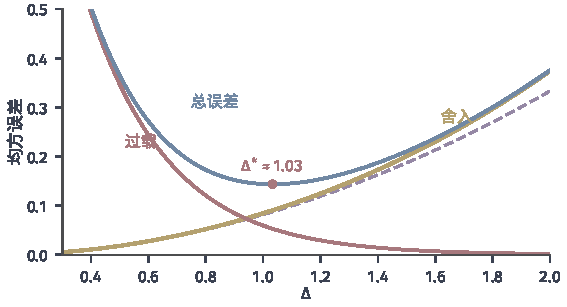
\includegraphics[width=96mm]{figures/07-probability/05-source-coding/matplotlib/quant-gran-overload/figure.pdf}
 \caption{$\operatorname{Laplace}(0,1)$读数、$N=8$的均匀量化器的平均失真随步长的变化，范围$L=4\Delta$。黄线为舍入部分的精确值，紫色虚线为其近似$\frac{\Delta^2}{12}\mathbb{P}(\lvert X\rvert\leq L)$，红线为过载部分~\eqref{eq:quant-laplace-overload}，蓝线为总和；红点为最优步长$\Delta^{*}\approx1.03$。}
 \label{fig:quant-gran-overload}
\end{BookInlineFigure}

\paragraph{点数的权衡}
增加点数时，最优步长与范围一起变化。表~\ref{tab:quant-uniform-points}列出对每个$N$搜索最优步长的结果。点数每加倍，最优范围大约增加$1.1$，而不是保持不变：为了让过载项$\mathrm{e}^{-L}$与舍入项$\Delta^{2}/12$同步减小，范围必须随点数缓慢变宽。所以步长缩小不到一半，每多一个比特，失真只降为原来的$0.35$左右，而不是理想的四分之一。

\begin{BookInlineTable}
 \centering
 \begin{tabular}{rrrrrr}
  \toprule
  $N$ & $\Delta^{*}$ & $L^{*}$ & 舍入 & 过载 & 总失真\\
  \midrule
  $4$ & $1.538$ & $3.08$ & $0.2020$ & $0.1906$ & $0.3926$\\
  $8$ & $1.034$ & $4.13$ & $0.0907$ & $0.0528$ & $0.1435$\\
  $16$ & $0.652$ & $5.22$ & $0.0357$ & $0.0150$ & $0.0507$\\
  $32$ & $0.396$ & $6.34$ & $0.0131$ & $0.0043$ & $0.0174$\\
  \bottomrule
 \end{tabular}
 \caption{$\operatorname{Laplace}(0,1)$读数的最优均匀量化器（定长索引）。舍入与过载为精确值；同样点数的Lloyd--Max量化器失真依次为$0.3524$、$0.1090$、$0.0307$、$0.0082$。}
 \label{tab:quant-uniform-points}
\end{BookInlineTable}

\paragraph{误差的尾部}
平均失真之外，有时还关心误差偶尔有多大。范围内的误差总不超过$\Delta/2$，超过$\Delta/2$的误差只能来自过载。对$s\geq\Delta/2$，$\lvert E\rvert>s$等价于$\lvert X\rvert>L-\Delta/2+s$，所以
\[
 \mathbb{P}\bigl(\lvert E\rvert>s\bigr)=\mathrm{e}^{-(L-\Delta/2+s)},\qquad s\geq\frac{\Delta}{2} .
\]
$N=8$、$\Delta=1$时，误差超过$0.5$的概率是$\mathrm{e}^{-4}=0.018$，超过$1$的概率是$\mathrm{e}^{-4.5}=0.011$，超过$2$的概率是$\mathrm{e}^{-5.5}=0.004$。误差没有上界，但它的尾部继承了读数的尾部。需要保证最坏误差时，只能加大范围或另外描述越界的读数。

\paragraph{误差与读数的关系}
误差$E=Q(X)-X$是读数的函数，给定读数，误差就完全确定。所以$E$与$X$不可能独立（除非$E$几乎必然为常数）。即使只看相关性，误差与读数一般也相关：若重构值都是质心，由第~\ref{sec:quant-nonuniform}节的正交性，$\mathbb{E}[EQ(X)]=0$，而$X=Q(X)-E$，于是
\[
 \mathbb{E}[XE]=\mathbb{E}[Q(X)E]-\mathbb{E}[E^{2}]=-D .
\]
又$\mathbb{E}[E]=0$，所以$\operatorname{Cov}(X,E)=-D\neq0$。

常用的“加性噪声模型”把量化写成$Q(X)=X+E$，并假定$E$与$X$独立、在$[-\Delta/2,\Delta/2]$上均匀分布。上面的讨论说明这只是一个近似：在高分辨率下，误差的分布接近均匀（图~\ref{fig:quant-error-shape}右图），与读数的相关系数$-\sqrt{D}/\sqrt{\operatorname{Var}(X)}$趋于零，用它估算平均失真是合理的；但在粗量化、有过载，或读数本身取值规则（例如总落在刻度附近、长时间停在同一个区间内）时，它会给出错误的结论。第~\ref{sec:quant-dither}节给出一种使这个模型精确成立的办法。

\paragraph{期望难以计算时}
上面的平均失真都由显式积分得到。分布或区域复杂时，例如向量量化的Voronoi区域，期望难以直接积分，可以用模拟的平均代替：独立地生成$n$个读数，计算误差平方的样本平均。它本身是期望的一个估计，有自己的随机误差，应当与量化误差分开报告。例如对$N=8$、$\Delta=1$的Laplace例子，用$n=10^{5}$个模拟读数（种子7），得到估计$0.1438$，标准误差约$0.0025$；精确值$0.1440$在其范围之内。模拟误差怎样随$n$缩小、怎样给出可靠的区间，见第~\ref{chap:monte-carlo-integration-error}章。

\paragraph{比较的前提}
比较两个量化器时，源分布、失真函数和描述资源必须相同。表~\ref{tab:quant-uniform-points}与图~\ref{fig:quant-operational}都遵守这一点：同一个Laplace读数、平方误差，横向比较时固定点数或固定平均码长。单纯增加点数总能降低误差，但同时增加存储、搜索与描述长度；说一个量化器“更好”，必须说明是在哪种资源下更好。

\subsection{抖动对误差的影响}
\label{sec:quant-dither}

确定性量化的误差由读数决定，这在某些场合是个实际问题。设读数长时间停在$x=0.3$附近，用步长$\Delta=1$、零为重构值的无穷均匀量化器~\eqref{eq:quant-midtread}，每次都报$0$，误差恒为$-0.3$。多次记录再平均也消除不了这个偏差，因为误差没有任何随机性可以被平均掉。能否让误差变成与读数无关的随机量？

\paragraph{减性抖动}
办法是在量化前给读数加一个随机扰动，并让解码器知道同一个扰动，重构时再把它减掉。设$U$与$X$独立，服从$[-\Delta/2,\Delta/2)$上的均匀分布。编码器量化$X+U$，传送索引；解码器取得同一个$U$的值（例如双方使用同一个伪随机数发生器和种子），输出
\begin{equation}
 \hat{X}=Q_{\Delta}(X+U)-U .
 \label{eq:quant-subtractive-dither}
\end{equation}
这称为\term{减性抖动}（subtractive dither），所加的扰动称为\term{抖动}（dither）。重构误差为
\[
 E=\hat{X}-X=Q_{\Delta}(X+U)-(X+U) ,
\]
也就是对$V=X+U$做舍入的误差。

先用$x=0.3$、$\Delta=1$手算三个扰动值。取$u=0.37$，$v=0.67$舍入到$1$，于是
\[
 \hat{x}=1-0.37=0.63,\qquad E=0.33 .
\]
取$u=-0.42$，$v=-0.12$舍入到$0$，于是
\[
 \hat{x}=0+0.42=0.42,\qquad E=0.12 .
\]
取$u=0.1$，$v=0.4$舍入到$0$，于是
\[
 \hat{x}=-0.1,\qquad E=-0.4 .
\]
同一个读数，误差随扰动变化，有正有负。

\paragraph{误差的分布}
为什么误差会均匀？固定$x$，$V=x+U$均匀分布在一个长度恰为$\Delta$的区间$[x-\Delta/2,x+\Delta/2)$上。这个区间恰好跨过一个刻度区间的边界，把它切成两段：左段舍入到一个刻度，右段舍入到下一个刻度。两段上的舍入误差$Q_{\Delta}(v)-v$各自扫过$[-\Delta/2,\Delta/2)$的一部分，拼起来恰好扫过一遍。图~\ref{fig:quant-dither-mechanism}画出$x=0.3$的情形。

\begin{BookInlineFigure}
 \centering
 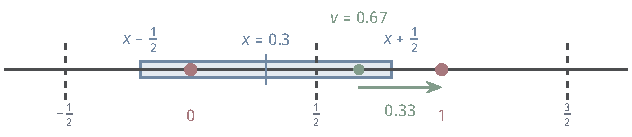
\includegraphics[width=107.1mm]{figures/07-probability/05-source-coding/tikz/quant-dither-mechanism/figure.pdf}
 \caption{减性抖动的机制，$\Delta=1$，$x=0.3$。浅蓝带是$V=x+U$的取值范围$[-0.2,0.8)$，红点是刻度$0$与$1$，虚线是区间边界。带中$[-0.2,0.5)$部分舍入到$0$，误差$-v$取遍$(-0.5,0.2]$；$[0.5,0.8)$部分舍入到$1$，误差$1-v$取遍$(0.2,0.5]$。绿点为$u=0.37$时的$v=0.67$，箭头长度是误差$0.33$。}
 \label{fig:quant-dither-mechanism}
\end{BookInlineFigure}

\begin{theorem}[减性抖动的误差]
\label{thm:quant-subtractive-dither}
设$Q_{\Delta}$为式~\eqref{eq:quant-midtread}的无穷均匀量化器，$U$服从$[-\Delta/2,\Delta/2)$上的均匀分布且与$X$独立。则式~\eqref{eq:quant-subtractive-dither}的重构误差$E=\hat{X}-X$服从$(-\Delta/2,\Delta/2]$上的均匀分布，并且与$X$独立。特别地，
\begin{equation}
 \mathbb{E}[E]=0,\qquad \mathbb{E}[E^{2}]=\frac{\Delta^{2}}{12} ,
 \label{eq:quant-dither-moments}
\end{equation}
对任何读数分布成立。
\end{theorem}

\begin{proof}
记$g(v)=Q_{\Delta}(v)-v$，它是周期为$\Delta$的函数，在$[k\Delta-\Delta/2,k\Delta+\Delta/2)$上等于$k\Delta-v$，取值于$(-\Delta/2,\Delta/2]$。于是$E=g(X+U)$。

先固定$x$，计算$g(x+U)$的分布。$x+U$在$I_x=[x-\Delta/2,x+\Delta/2)$上均匀分布，密度为$1/\Delta$。对$(-\Delta/2,\Delta/2]$中的Borel集$B$，
\[
 \mathbb{P}\bigl(g(x+U)\in B\bigr)=\frac{1}{\Delta}\,\lambda\bigl(\{v\in I_x:g(v)\in B\}\bigr) ,
\]
$\lambda$为长度。$I_x$长度恰为$\Delta$，按刻度区间的边界把它切成至多两段，每段上$g(v)=k\Delta-v$是斜率为$-1$的平移，保持长度。两段的像拼起来恰为$(-\Delta/2,\Delta/2]$，互不重叠，因为$g$的周期为$\Delta$，长度为$\Delta$的区间上每个误差值恰好出现一次。所以上式右边等于$\lambda(B)/\Delta$，与$x$无关。

再证独立性。$X$与$U$独立，$(X,U)$的联合分布是乘积分布。对Borel集$A$与$B$，由Fubini定理先对$U$积分，
\[
 \mathbb{P}(X\in A,\ E\in B)=\int_{A}\mathbb{P}\bigl(g(x+U)\in B\bigr)\,P_X(\mathrm{d}x)=P_X(A)\,\frac{\lambda(B)}{\Delta} .
\]
取$A=\mathbb{R}$，得$E$服从均匀分布；于是上式就是$\mathbb{P}(X\in A)\mathbb{P}(E\in B)$，$E$与$X$独立。式~\eqref{eq:quant-dither-moments}是均匀分布的均值与二阶矩。
\end{proof}

定理把加性噪声模型从近似变成了精确：$\hat{X}=X+E$，$E$与$X$独立且均匀。条件也说得很清楚：抖动必须恰好在一个步长上均匀，必须与读数独立，解码器必须减去同一个抖动，并且量化器不能过载。最后一条对无穷刻度自然成立；若刻度只覆盖$[-L,L]$，则需要$\lvert X\rvert\leq L-\Delta/2$，使$X+U$不越出范围。

回到$x=0.3$的例子。不加抖动时误差恒为$-0.3$，平方误差$0.09$；加减性抖动后，误差的均值为$0$、均方为$\tfrac1{12}\approx0.083$。图~\ref{fig:quant-dither-mse}右图用$20000$个抖动值（种子4）模拟了这个读数的误差：直方图在$[-0.5,0.5]$上是平的，样本均值约为$0.0004$，均方约为$0.0831$。

\paragraph{代价与资源}
抖动并不减小平均失真，它改变的是误差的结构。对一个读数分布，不加抖动的平均失真可能比$\Delta^{2}/12$小，也可能大。例如Laplace读数、$\Delta=1$时，不加抖动的无穷均匀量化器平均失真为$0.0810$，略小于减性抖动的$0.0833$；若读数总落在刻度上，不加抖动的误差为零，加抖动反而得到$\tfrac1{12}$。换来的好处是：误差与读数独立、无偏，多次独立抖动的记录取平均时误差会被平均掉。

这个方案还用到了额外的资源。给定$U=u$时，编码器仍只发送有限或可数个索引之一，重构值落在平移后的刻度$\{k\Delta-u\}$上；但随着$u$变化，所有可能的重构值铺满了整条实轴，不再是第~\ref{sec:quant-model}节意义下的有限码本。它依赖编码器与解码器共享同一个随机数，这是一种边信息。所以减性抖动是量化模型的一个扩展，与普通量化器比较时，要把共享扰动的要求一并计入。

\paragraph{非减性抖动}
若解码器拿不到抖动，只能输出$Q_{\Delta}(X+U)$，称为\term{非减性抖动}（non-subtractive dither）。这时误差不再与读数独立。固定读数$x=k\Delta+s$，$0\leq s<\Delta$，量化输出只可能是$k\Delta$或$(k+1)\Delta$；后者发生当且仅当$U\geq\Delta/2-s$，概率为$s/\Delta$。于是给定读数的条件均值为
\[
 \mathbb{E}\bigl[Q_{\Delta}(x+U)\bigr]=k\Delta+\frac{s}{\Delta}\Delta=x ,
\]
输出是无偏的。条件均方误差为
\[
 \frac{s}{\Delta}(\Delta-s)^{2}+\Bigl(1-\frac{s}{\Delta}\Bigr)s^{2}=s(\Delta-s) ,
\]
它随读数在$0$与$\Delta^{2}/4$之间变化：读数在刻度上时为$0$，在两刻度正中时达到$\Delta^{2}/4$。若$s$在$[0,\Delta)$上均匀，平均为$\Delta^{2}/6$，是减性抖动的两倍。

\begin{BookInlineFigure}
 \centering
 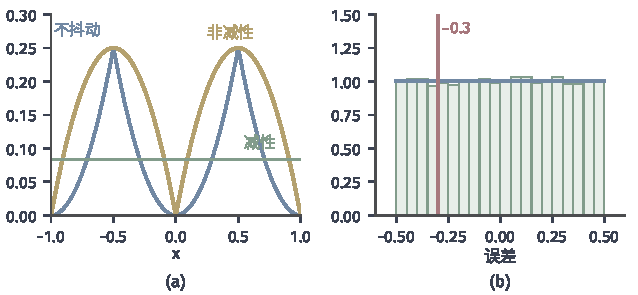
\includegraphics[width=108mm]{figures/07-probability/05-source-coding/matplotlib/quant-dither-mse/figure.pdf}
 \caption{$\Delta=1$的无穷均匀量化器在三种方式下的误差。(a) 给定读数$x$的条件均方误差：蓝线为不加抖动$(x-Q_1(x))^2$，绿线为减性抖动$\frac1{12}$，黄线为非减性抖动$s(1-s)$，$s=x-\lfloor x\rfloor$。(b) $x=0.3$时减性抖动的误差，$20000$个抖动值（种子4）的直方图（浅绿）与均匀密度（蓝线）；红线为不加抖动时的固定误差$-0.3$。}
 \label{fig:quant-dither-mse}
\end{BookInlineFigure}

图~\ref{fig:quant-dither-mse}左图把三种方式放在一起。不加抖动时，条件均方误差在刻度上为零、在刻度中点达到$\Delta^{2}/4$，形状完全由读数决定；非减性抖动消除了偏差，但条件均方误差仍随读数起伏，而且整体更大；只有减性抖动使条件均方误差与读数无关。三者的差别在于误差中有多少成分由读数决定，而这取决于解码器知道多少关于扰动的信息。


\section{本章小结}
\label{sec:quant-summary}

本章开头问：每个Laplace读数只存2个比特时，4个代表值放在哪里、读数怎样归属、平均误差多大。答案依次是：从均匀刻度出发，平均失真为$0.514$；按两条必要条件交替改进，得到阈值$\pm1.594$、重构值$\pm0.594$与$\pm2.594$，平均失真降到$0.352$；若允许变长记录，同一量化器的索引平均只需$1.805$ bit，而改用均匀刻度配合熵编码，在相近的平均长度下平均失真可以降到$0.21$左右。

\paragraph{三样东西决定三件事}
一个量化器由区域与重构值组成，它们共同决定平均失真$D(Q)$；索引的编码方式决定平均描述长度；是否加入共享的随机扰动，决定误差与读数之间的关系。三者分工不同：无损的索引编码不改变重构值，从而不改变失真；减性抖动不减小平均失真，只改变误差的结构。

\paragraph{平方误差下的两条条件}
固定区域时，最好的重构值是区域的质心，这来自平行轴恒等式~\eqref{eq:quant-parallel-axis}，也说明此时量化输出是给定索引下的条件期望；固定重构值时，最好的区域是最近邻区域，标量时阈值取中点，向量时得到Voronoi区域。最优量化器必须满足这两条，但满足它们的量化器未必最优。Lloyd--Max算法及其向量推广交替执行两步，平均失真单调不增，可能停在局部最优，结果依赖初值。

\paragraph{构造之间的比较}
本章的各种构造分别改变量化的不同环节，作用与代价各不相同。

\begin{BookInlineTable}
 \centering
 \begin{tabular}{lll}
  \toprule
  构造 & 得到什么 & 代价\\
  \midrule
  均匀量化 & 编码最简单 & 不适应分布，需饱和\\
  Lloyd--Max量化 & 按分布调整区间 & 需知道分布，局部最优\\
  向量量化 & 利用相关与形状 & 码本规模$2^{dR}$\\
  索引的熵编码 & 平均长度近$H(J)$ & 变长记录，需码表\\
  熵约束量化 & 按平均码长设计 & 目标含码长项\\
  减性抖动 & 误差独立于读数 & 共享随机数\\
  \bottomrule
 \end{tabular}
 \caption{本章各种构造的作用与代价。}
 \label{tab:quant-summary}
\end{BookInlineTable}

表~\ref{tab:quant-summary}汇总了各种构造。比较它们时，必须固定同一个源分布、同一个失真函数和同一种描述资源：重构点数、定长索引长度与平均索引长度是三种不同的预算，在一种预算下最好的方案，在另一种预算下未必最好。

\paragraph{误差的结构}
有限范围的均匀量化把误差分成两部分：范围内的舍入误差不超过半个步长，高分辨率下约为$\Delta^{2}/12$乘以范围内的概率；范围外的过载误差无界，其大小与尾部概率由读数的尾部决定。步长和范围的选择是这两部分之间的权衡，点数增加时范围也必须随之变宽。确定性量化的误差是读数的函数，“独立均匀噪声”只是高分辨率下的近似；只有在减性抖动下，它才精确成立。

\paragraph{有限方案与渐近极限}
本章的所有方案都是有限的：给定维数和点数，可以执行，也可以算出代价。它们不回答一个更根本的问题：允许把任意长的读数块放在一起描述时，给定每读数的比特数，平均失真最低能到多少。第~\ref{chap:rate-distortion}章用重构条件分布上的优化刻画这一极限，并把本章的有限量化器放到同一个标准下，衡量它们与极限之间的差距。


\chapter{率失真}
\label{chap:rate-distortion}

一个观测站每天只记录“下雨”或“不下雨”，多年统计中下雨的天数约占$30\%$，各天可近似看成相互独立。按第~\ref{chap:lossless-coding}章，若要求每天的记录都被准确还原，长期平均每天至少需要$h_2(0.3)\approx0.881$\,bit，这里$h_2$是以bit计的二元熵。现在放宽要求：允许接收方弄错大约$10\%$的天数。每天还需要多少bit？是直接按$0.881\times0.9$打个折扣，还是能省得更多？

连续取值的信源也有同样的问题。一个标准高斯测量值不可能用有限个bit精确记录，第~\ref{chap:quantization}章用有限个重构值把它装进格子，例如每个值用$1$\,bit的最优两点量化器，均方误差约为$0.363$。这个误差是$1$\,bit能做到的最好结果吗？如果把许多测量值合成一块统一描述，同样每值$1$\,bit，误差最低能降到多少？

这两个问题都在问：给定信源规律和失真标准，平均每个源符号至少需要多少描述。本章先在长块编码中把“可以做到”定义清楚，得到一个由所有方案决定的极限。然后把它与一个只涉及单个符号的优化问题联系起来：在平均失真不超过预算的随机重构规律中，找使互信息最小的一个。这个优化的最小值称为信息率失真函数，率失真编码定理证明它恰好等于长块编码的极限。

有了这个等式，计算就有了两条路。对二元信源与高斯信源，可以先证明一个对所有重构规律成立的信息下界，再构造一个达到它的规律，得到闭式解；开头的两个问题都由此回答。对一般的有限概率表，用Blahut–Arimoto交替算法数值求解。全章以$\operatorname{Bern}(0.3)$信源和Hamming失真为贯穿例子，用标准高斯信源和平方失真评价有限量化器；信息量一律以bit计量。

\section{块重构模型}
\label{sec:rd-block-model}

“至少需要多少描述”要先说清比较的是哪些方案。第~\ref{chap:quantization}章的量化器一次处理一个值，而开头的问题允许把许多天的记录合在一起描述。合在一起之后，一个消息对应一整块重构，失真也要按整块来算。这一节把块编码、码率与失真写成确定的对象，再用块长增长的方案序列定义什么叫“可以做到”。

\paragraph{信源与失真}
设信源依次产生$X_1,X_2,\dots$，它们相互独立，都服从取值空间$\mathcal{X}$上的同一分布$P_X$，这样的信源称为\term{无记忆信源}（memoryless source）。接收方用\term{重构字母表}（reconstruction alphabet）$\hat{\mathcal{X}}$中的值重构，它不必与$\mathcal{X}$相同。与第~\ref{chap:quantization}章一样，重构的好坏由一个失真函数$d:\mathcal{X}\times\hat{\mathcal{X}}\to[0,\infty)$衡量，$d(x,\hat{x})$是把$x$重构成$\hat{x}$的代价。

本章常用两种失真。二元或有限字母表上取$\mathcal{X}=\hat{\mathcal{X}}$，并取
\begin{equation}
  d(x,\hat{x})=\mathbf{1}_{\{x\neq\hat{x}\}},
  \label{eq:rd-hamming}
\end{equation}
它只记对错，称为\term{Hamming失真}（Hamming distortion），平均失真就是重构错误的比例。实值信源取平方失真$d(x,\hat{x})=(x-\hat{x})^{2}$，平均失真就是均方误差。

把$n$个符号合成一块$x^{n}=(x_1,\dots,x_n)$，重构块记为$\hat{x}^{n}$。块的失真取逐符号失真的平均：
\begin{equation}
  d_n(x^{n},\hat{x}^{n})=\frac{1}{n}\sum_{i=1}^{n}d(x_i,\hat{x}_i).
  \label{eq:rd-block-distortion}
\end{equation}
这种按符号相加的失真称为可分失真。取平均而不取总和，是为了让不同块长的方案在“每个符号的失真”上可以直接比较。

\paragraph{块编码}
发送方看到整块$x^{n}$后，只向接收方传一个消息编号；接收方只凭这个编号输出整块重构。图~\ref{fig:rd-block-scheme}画出了这条链路。

\begin{definition}[块编码与码率]
\label{def:rd-block-code}
一个$(n,M)$\term{率失真码}（rate-distortion code）由编码器$f_n:\mathcal{X}^{n}\to\{1,\dots,M\}$与解码器$g_n:\{1,\dots,M\}\to\hat{\mathcal{X}}^{n}$组成。$g_n$的$M$个输出称为码字，它们的集合称为码本。码的码率与期望失真分别是
\begin{equation}
  R=\frac{\log_2M}{n},\qquad
  \mathbb{E}\bigl[d_n\bigl(X^{n},g_n(f_n(X^{n}))\bigr)\bigr],
  \label{eq:rd-rate}
\end{equation}
码率的单位是bit每源符号。
\end{definition}

\begin{BookInlineFigure}
  \centering
  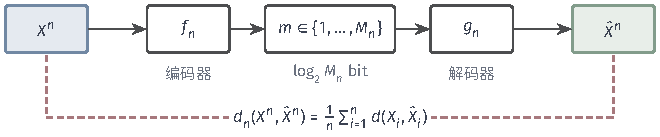
\includegraphics[width=112mm]{figures/07-probability/05-source-coding/tikz/rd-block-scheme/figure.pdf}
  \caption{块重构模型。蓝框是长度为$n$的源块，绿框是重构块。编码器$f_n$把整块映射成$M_n$个编号之一，编号要用约$\log_2M_n$\,bit描述；解码器$g_n$只凭编号输出整块重构。红色虚线表示按式~\eqref{eq:rd-block-distortion}逐符号比较两块。}
  \label{fig:rd-block-scheme}
\end{BookInlineFigure}

$M$不必是$2$的幂。把很多个块连起来发送时，$k$个编号一共有$M^{k}$种组合，用$\lceil k\log_2M\rceil$个bit就能区分，所以$\log_2M$正是每块平均要付出的bit数，除以$n$得到每个源符号的份额。码率只数编号的个数，不涉及编号怎样写成二进制串，也不对编号再作第~\ref{chap:lossless-coding}章的变长压缩；本章所说的码率都是这种固定描述的码率。

码本一旦固定，编码器怎么选最好？对每个$x^{n}$，期望失真中它的那一项是$d_n(x^{n},g_n(f_n(x^{n})))$，只依赖它被送到哪个码字。把每个$x^{n}$送到使$d_n$最小的码字，就同时使每一项最小，期望失真自然最小。所以在给定码本时，最优编码器就是\term{最近码字编码器}（nearest-codeword encoder），一个码本就决定了整个码。这与第~\ref{chap:quantization}章固定重构值后按最近邻划分区域是同一件事，只是“点”换成了整块。

\paragraph{几个简单的码}
回到开头的雨天记录：$X_i\sim\operatorname{Bern}(0.3)$，$1$表示下雨，用Hamming失真。最省的做法是不传任何信息，接收方一律猜“不下雨”。这时$M=1$，码率为$0$，错误比例是下雨的概率：
\[
  R=0,\qquad \mathbb{E}d_n=\mathbb{P}(X_i=1)=0.3 .
\]
另一个极端是逐天照传，$n=1$，$M=2$，码率为$1$，失真为$0$。

块长$n=3$时，可以只用两个码字$\{000,111\}$。在最近码字编码下，一块里$1$的个数$K$不超过$1$时送$000$，否则送$111$，这就是多数表决。$K\sim\operatorname{Bin}(3,0.3)$，
\[
  \begin{gathered}
  \mathbb{P}(K=0)=0.343,\quad \mathbb{P}(K=1)=0.441,\\
  \mathbb{P}(K=2)=0.189,\quad \mathbb{P}(K=3)=0.027 .
  \end{gathered}
\]
$K=1$或$K=2$时恰好错一位，$K=0$或$3$时不错，所以
\[
  \mathbb{E}d_3=\frac{1}{3}\,(0.441+0.189)=0.21,\qquad R=\frac{\log_2 2}{3}=\frac13 .
\]

图~\ref{fig:rd-hamming-cube}把这个码画在三维立方体上。八个顶点是全部源块，相邻顶点只差一位，所以沿棱走一步就是一个Hamming错误。蓝色顶点被送到$000$，黄色顶点被送到$111$，两块区域就是两个码字的最近邻区域。

\begin{BookInlineFigure}
  \centering
  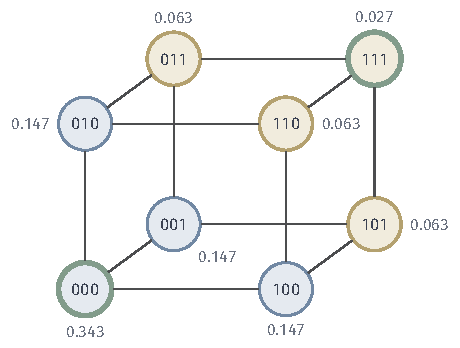
\includegraphics[width=78mm]{figures/07-probability/05-source-coding/tikz/rd-hamming-cube/figure.pdf}
  \caption{块长$3$的码本$\{000,111\}$。立方体的八个顶点是全部源块，旁边的数是它在$\operatorname{Bern}(0.3)$信源下的概率；绿色粗圈是两个码字。蓝色顶点距$000$更近，黄色顶点距$111$更近。蓝色区域的概率是$0.343+3\times0.147=0.784$，其中三个只有一位为$1$的顶点各贡献一个错误。}
  \label{fig:rd-hamming-cube}
\end{BookInlineFigure}

再换一个码本$\{000,100,010,001\}$，$M=4$，码率$\tfrac23$。$K\leq1$的块都能精确重构；$K=2$时最近码字错一位，$K=3$时错两位：
\[
  \mathbb{E}d_3=\frac{1}{3}\,(0.189\times1+0.027\times2)=0.081,\qquad R=\frac{\log_2 4}{3}=\frac23 .
\]
它把码字都放在概率大的地方，利用了“下雨少”这一规律。

还有一种不需要新码本的组合办法。把长块的前一部分符号逐个照传、其余部分一律猜$0$：照传的比例为$\lambda$时，码率为$\lambda$，失真为$0.3(1-\lambda)$。这种在不同方案之间按比例分配符号的做法称为\term{分时}（time sharing），它在码率—失真平面上连出两点之间的线段。

图~\ref{fig:rd-simple-codes}把这些码画在一起。重复码在分时线段的上方：同样码率$\tfrac13$，分时的失真只有$0.2$。四码字的码在线段下方，同样码率$\tfrac23$，分时的失真是$0.1$，它做到了$0.081$。可见简单的组合并不总是最好，块长与码本的选择都影响结果。我们要找的是所有方案都越不过的那条边界。

\begin{BookInlineFigure}
  \centering
  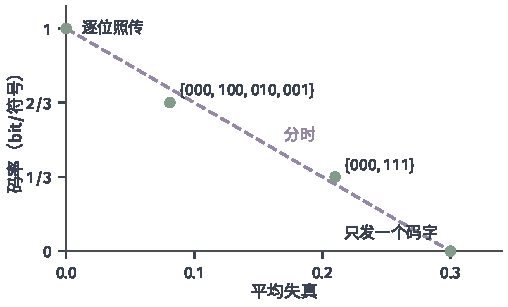
\includegraphics[width=86mm]{figures/07-probability/05-source-coding/matplotlib/rd-simple-codes/figure.pdf}
  \caption{$\operatorname{Bern}(0.3)$信源在Hamming失真下几个简单码的码率与平均失真（绿点）：只发一个码字、逐位照传、块长$3$的重复码$\{000,111\}$和码本$\{000,100,010,001\}$。紫色虚线是前两个方案之间的分时。}
  \label{fig:rd-simple-codes}
\end{BookInlineFigure}

\paragraph{渐近可达性}
单个块长的码受到整数效应的牵制：$M$只能是整数，码字只能放在格点上。为了得到一个干净的极限，我们看块长不断增长的一列码。

\begin{definition}[可达码率失真对]
\label{def:rd-achievable}
若对每个$n\geq1$都有一个$(n,M_n)$码，使
\begin{equation}
  \limsup_{n\to\infty}\frac{\log_2M_n}{n}\leq R,\qquad
  \limsup_{n\to\infty}\mathbb{E}\bigl[d_n\bigl(X^{n},g_n(f_n(X^{n}))\bigr)\bigr]\leq D,
  \label{eq:rd-achievable}
\end{equation}
则称$(R,D)$为\term{可达码率失真对}（achievable rate-distortion pair）。对给定的$D$，所有使$(R,D)$可达的$R$的下确界记为$R_{\mathrm{op}}(D)$，称为\term{操作率失真函数}（operational rate-distortion function）。
\end{definition}

定义中两个上极限分别留出了余地：码率可以比$R$稍大，只要最终不超过$R$；失真也一样。有限块长的码不在定义之内，它们只是这一列中的成员。若$(R,D)$可达，那么任何更大的$R'$与$D'$也可达，所以可达的点组成码率—失真平面中一块向右上方延伸的区域，$R_{\mathrm{op}}$是它的下边界。

\paragraph{三种失真要求}
“失真不超过$D$”还可以有别的读法，它们给出不同的极限，需要事先分清。式~\eqref{eq:rd-achievable}用的是期望失真：对源块的分布平均以后不超过$D$，个别块的失真可以很大。第二种是逐块保证，要求每一个可能的源块都满足$d_n\leq D$。第三种是超额失真概率要求，即
\[
  \mathbb{P}\bigl(d_n(X^{n},\hat{X}^{n})>D\bigr)\to0 ,
\]
允许失真超标，但超标的概率要趋于零。

若失真有上界$d_{\max}=\max_{x,\hat{x}}d(x,\hat{x})<\infty$，后两种要求都强于期望失真要求。把期望按是否超标分成两部分：
\[
  \mathbb{E}d_n\leq D\cdot\mathbb{P}(d_n\leq D)+d_{\max}\,\mathbb{P}(d_n>D)
  \leq D+d_{\max}\,\mathbb{P}(d_n>D).
\]
超额失真概率趋零时右端趋于$D$，所以满足第三种要求的码列也满足期望失真要求。反过来不成立：对一半的块照传、另一半一律猜$0$的码，期望失真可以很小，超标概率却始终是$\tfrac12$。

逐块保证则可能贵得多。仍看Hamming失真与$0<D<\tfrac12$。一个码字能“照顾”到的源块，是与它相差不超过$nD$位的那些，个数至多为$\sum_{k\leq nD}\binom{n}{k}$。对$t=D/(1-D)\leq1$，二项展开给出
\[
  1=\sum_{k=0}^{n}\binom{n}{k}D^{k}(1-D)^{n-k}
  \geq\sum_{k\leq nD}\binom{n}{k}(1-D)^{n}t^{k}
  \geq\sum_{k\leq nD}\binom{n}{k}(1-D)^{n}t^{nD},
\]
这里第二个不等号用了$k\leq nD$与$t\leq1$。而$(1-D)^{n}t^{nD}=D^{nD}(1-D)^{n-nD}=2^{-nh_2(D)}$，其中$h_2(t)=-t\log_2t-(1-t)\log_2(1-t)$是二元熵。于是
\[
  \sum_{k\leq nD}\binom{n}{k}\leq2^{nh_2(D)} .
\]

要照顾到全部$2^{n}$个源块，码字个数必须满足$M_n\cdot2^{nh_2(D)}\geq2^{n}$，即
\[
  \frac{\log_2M_n}{n}\geq1-h_2(D).
\]
这个界与下雨的概率$0.3$完全无关：概率再小的块也必须被照顾。取$D=0.1$，右端为$1-h_2(0.1)\approx0.531$\,bit。第~\ref{sec:rd-binary}节将算出期望失真标准下只需约$0.412$\,bit，差别就来自是否允许罕见的块失真偏大。

逐块保证适合要防最坏情况的场合，超额失真概率适合要控制“几乎每块”的场合。本章以期望失真为共同标准，它与平均码长一样关心长期平均表现，也是第~\ref{chap:quantization}章评价量化器的标准。


\section{信息率失真函数}
\label{sec:rd-information-rd}

$R_{\mathrm{op}}(D)$的定义涉及所有块长、所有码本，无法直接计算。我们需要一个只看单个符号就能算的量，并且它要与码的描述能力挂钩。互信息正好起这个作用。

设$(n,M)$码的重构块为$\hat{X}^{n}=g_n(f_n(X^{n}))$。它由编号决定，至多取$M$个值，所以它能携带的关于$X^{n}$的信息有限：
\[
  I(X^{n};\hat{X}^{n})\leq H(\hat{X}^{n})\leq\log_2M=nR .
\]
第一个不等号来自
\[
  I(X^{n};\hat{X}^{n})=H(\hat{X}^{n})-H(\hat{X}^{n}\mid X^{n})
\]
与条件熵非负，第二个是取$M$个值的变量熵不超过$\log_2M$。所以码率至少要容纳重构与源之间的互信息。重构必须足够接近源，这又迫使互信息不能太小。下面在单个符号上精确地表述这种张力：失真不超过$D$时，互信息最少是多少。

这里沿用第~\ref{chap:information-measures}章的熵、条件熵与互信息，只把对数换成以$2$为底，数值都除以$\ln2$，单位从nat变成bit。有限字母表上，
\[
  I(X;\hat{X})=\sum_{x,\hat{x}}p(x,\hat{x})\log_2\frac{p(x,\hat{x})}{p(x)\,r(\hat{x})},
\]
其中$r$是$\hat{X}$的分布；它就是联合分布相对边缘乘积的KL散度，非负，且为零当且仅当$X$与$\hat{X}$独立。

\subsection{重构条件分布}
\label{sec:rd-test-channels}

单个符号上，一个“重构规律”就是给定源值$x$时，重构值怎样选择。允许这种选择带有随机性，用条件分布描述它。

设$\mathcal{X}$与$\hat{\mathcal{X}}$是有限集，$p(x)=P_X(\{x\})$。一个\term{测试信道}（test channel）是一族条件概率$q(\hat{x}\mid x)\geq0$，对每个$x$有$\sum_{\hat{x}}q(\hat{x}\mid x)=1$。它与源分布一起确定联合分布$p(x)q(\hat{x}\mid x)$，重构的边缘分布是
\begin{equation}
  r_q(\hat{x})=\sum_{x}p(x)\,q(\hat{x}\mid x).
  \label{eq:rd-output-marginal}
\end{equation}
把$q$看作一个随机的“重构器”：输入$x$，按$q(\cdot\mid x)$抽一个$\hat{x}$输出。它的平均失真与互信息分别是
\begin{equation}
  \mathbb{E}d(X,\hat{X})=\sum_{x,\hat{x}}p(x)\,q(\hat{x}\mid x)\,d(x,\hat{x}),
  \label{eq:rd-test-distortion}
\end{equation}
\begin{equation}
  I(P_X,q)=\sum_{x,\hat{x}}p(x)\,q(\hat{x}\mid x)\log_2\frac{q(\hat{x}\mid x)}{r_q(\hat{x})}.
  \label{eq:rd-test-information}
\end{equation}
式~\eqref{eq:rd-test-information}中约定$0\log_20=0$；若$p(x)q(\hat{x}\mid x)>0$，则$r_q(\hat{x})>0$，分母不会为零。

\begin{definition}[信息率失真函数]
\label{def:rd-information-rd}
给定源分布$P_X$与失真函数$d$，对$D\geq0$令
\begin{equation}
  R(D)=\inf\Bigl\{I(P_X,q):\ q\text{为测试信道},\ \mathbb{E}d(X,\hat{X})\leq D\Bigr\},
  \label{eq:rd-information-rd}
\end{equation}
约定空集的下确界为$+\infty$。$R(D)$称为\term{信息率失真函数}（information rate-distortion function），单位是bit每源符号。
\end{definition}

式~\eqref{eq:rd-information-rd}的优化变量只有测试信道$q$。源分布$P_X$是给定的，不参与优化；改变的只是“看到$x$以后怎样重构”。下一部分研究信道时问题方向相反：信道的条件分布固定，改变的是输入分布。两个问题都优化互信息，但一个求最小、一个求最大，变量也不同。

测试信道是一个理论对象，不是编码器。真正的编码器看到整块源符号，确定地输出一个编号；测试信道只作用在单个符号上，并且允许抛硬币。它在本章有两个用处：在第~\ref{sec:rd-coding-theorem}节的下界证明中，任意块编码都会诱导出一个测试信道；在可达性证明中，最优测试信道指导怎样随机生成码本。$R(D)$与$R_{\mathrm{op}}(D)$相等是需要证明的定理，现在只把$R(D)$当作一个优化问题来研究。

一般的取值空间中，测试信道是从$\mathcal{X}$到$\hat{\mathcal{X}}$的Markov核（第~\ref{chap:conditional-distributions}章），互信息用联合分布相对边缘乘积的KL散度定义，允许取$+\infty$，式~\eqref{eq:rd-information-rd}的写法不变。本节余下部分先在有限字母表上讨论，一般情形放在第~\ref{sec:rd-feasible-range}节末尾。

\paragraph{三个测试信道}
仍取$X\sim\operatorname{Bern}(0.3)$与Hamming失真。第一个测试信道不看输入，一律输出$0$。这时$\hat{X}$是常数，与$X$独立，
\[
  I=0,\qquad \mathbb{E}d=\mathbb{P}(X=1)=0.3 .
\]

第二个测试信道以概率$0.1$把输入翻转：$q(1\mid0)=q(0\mid1)=0.1$。平均失真正好是翻转概率$0.1$。由式~\eqref{eq:rd-output-marginal}，
\[
  r_q(1)=0.7\times0.1+0.3\times0.9=0.34 .
\]
给定$X$时$\hat{X}$的熵是$h_2(0.1)$，于是
\[
  I=H(\hat{X})-H(\hat{X}\mid X)=h_2(0.34)-h_2(0.1)\approx0.9248-0.4690=0.4558 .
\]

第三个测试信道取$q(1\mid0)=\tfrac1{28}$，$q(0\mid1)=\tfrac14$：常见的$0$几乎不动，罕见的$1$有四分之一被改成$0$。平均失真仍然是
\[
  \mathbb{E}d=0.7\times\frac{1}{28}+0.3\times\frac14=0.025+0.075=0.1 .
\]
重构边缘为
\[
  r_q(1)=0.7\times\frac1{28}+0.3\times\frac34=0.25 .
\]

给定$X=0$与$X=1$时$\hat{X}$的熵分别是$h_2(\tfrac1{28})$与$h_2(\tfrac14)$，按$p(x)$平均得条件熵，于是
\[
  I=h_2(0.25)-0.7\,h_2\Bigl(\frac1{28}\Bigr)-0.3\,h_2\Bigl(\frac14\Bigr)
  \approx0.8113-0.1556-0.2434=0.4123 .
\]
同样的失真，第三个信道比第二个少用了约$0.044$\,bit的信息。它把错误集中在罕见符号上：把一个$1$改成$0$让重构更“像”最常见的结果，重构本身更可预测，需要的描述更少。第~\ref{sec:rd-binary}节将证明$0.4123$正是$R(0.1)$。

图~\ref{fig:rd-test-channel-cloud}把所有二元测试信道一次画出来。$q(1\mid0)$与$q(0\mid1)$各取网格上的值，每个测试信道对应一个点（平均失真，互信息）。$R(D)$就是这团点云的下边界：在竖线$D$的左侧所有点中，最低的高度。

\begin{BookInlineFigure}
  \centering
  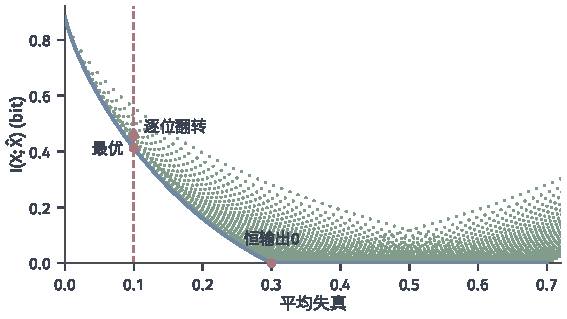
\includegraphics[width=96mm]{figures/07-probability/05-source-coding/matplotlib/rd-test-channel-cloud/figure.pdf}
  \caption{$\operatorname{Bern}(0.3)$信源与Hamming失真下全部二元测试信道的平均失真与互信息。绿点：$q(1\mid0)$与$q(0\mid1)$各取$0,\tfrac1{60},\dots,1$共$61\times61$个组合。蓝线是点云的下边界$R(D)$，其公式在第~\ref{sec:rd-binary}节导出。红点依次是以$0.1$翻转的测试信道、$D=0.1$时的最优测试信道和恒输出$0$；红色虚线是$D=0.1$。}
  \label{fig:rd-test-channel-cloud}
\end{BookInlineFigure}

\subsection{单调性与凸性}
\label{sec:rd-convexity}

点云的下边界看上去单调下降、向下凸。单调性只需比较可行集合。

失真预算放宽时，满足$\mathbb{E}d\leq D$的测试信道都满足$\mathbb{E}d\leq D'$，其中$D<D'$。在更大的集合上取下确界只会更小，所以$R(D')\leq R(D)$，$R$非增。

凸性来自互信息对测试信道的凸性。证明要用一个关于两组非负数的不等式，它把KL散度非负的论证推广到未归一化的数组。

\begin{lemma}[对数和不等式]
\label{lem:rd-log-sum}
设$a_1,\dots,a_k\geq0$，$b_1,\dots,b_k>0$，$a=\sum_ia_i$，$b=\sum_ib_i$。则
\begin{equation}
  \sum_{i=1}^{k}a_i\log_2\frac{a_i}{b_i}\geq a\log_2\frac{a}{b},
  \label{eq:rd-log-sum}
\end{equation}
约定$0\log_20=0$。
\end{lemma}

\begin{proof}
$a=0$时两边都为$0$。设$a>0$，记$\phi(t)=t\log_2t$（$\phi(0)=0$），它在$[0,\infty)$上凸，因为$t>0$时$\phi''(t)=1/(t\ln2)>0$。左端可以写成
\[
  \sum_{i}a_i\log_2\frac{a_i}{b_i}=b\sum_{i}\frac{b_i}{b}\,\phi\Bigl(\frac{a_i}{b_i}\Bigr).
\]
权重$b_i/b$非负且和为$1$，由Jensen不等式，
\[
  \sum_{i}\frac{b_i}{b}\,\phi\Bigl(\frac{a_i}{b_i}\Bigr)\geq\phi\Bigl(\sum_{i}\frac{b_i}{b}\cdot\frac{a_i}{b_i}\Bigr)=\phi\Bigl(\frac{a}{b}\Bigr)=\frac{a}{b}\log_2\frac{a}{b}.
\]
两边乘以$b$即得式~\eqref{eq:rd-log-sum}。
\end{proof}

\begin{lemma}[互信息对测试信道的凸性]
\label{lem:rd-mi-convex}
固定有限字母表上的源分布$P_X$。对测试信道$q_1,q_2$与$\lambda\in[0,1]$，令$q_\lambda=\lambda q_1+(1-\lambda)q_2$，则
\begin{equation}
  I(P_X,q_\lambda)\leq\lambda\,I(P_X,q_1)+(1-\lambda)\,I(P_X,q_2).
  \label{eq:rd-mi-convex}
\end{equation}
\end{lemma}

\begin{proof}
$q_\lambda$的每一行仍是概率分布，所以它是测试信道。固定一对$(x,\hat{x})$，记
\[
  a_j=p(x)\,q_j(\hat{x}\mid x),\qquad b_j=p(x)\,r_{q_j}(\hat{x}),\qquad j=1,2 .
\]
由式~\eqref{eq:rd-output-marginal}，$r_q$对$q$是线性的，所以$q_\lambda$对应的两个量正好是$\lambda a_1+(1-\lambda)a_2$与$\lambda b_1+(1-\lambda)b_2$。

式~\eqref{eq:rd-test-information}在$(x,\hat{x})$处的项是$a\log_2(a/b)$的形式。对两项$\lambda a_1,(1-\lambda)a_2$与$\lambda b_1,(1-\lambda)b_2$用引理~\ref{lem:rd-log-sum}（分母为零的项分子也为零，可以略去），得
\[
  \bigl(\lambda a_1+(1-\lambda)a_2\bigr)\log_2\frac{\lambda a_1+(1-\lambda)a_2}{\lambda b_1+(1-\lambda)b_2}
  \leq\lambda\,a_1\log_2\frac{a_1}{b_1}+(1-\lambda)\,a_2\log_2\frac{a_2}{b_2}.
\]
对所有$(x,\hat{x})$求和，左端是$I(P_X,q_\lambda)$，右端是式~\eqref{eq:rd-mi-convex}的右端。
\end{proof}

\begin{theorem}[$R(D)$的单调性与凸性]
\label{thm:rd-convex}
有限字母表上，$R$在$[0,\infty)$上非增。在$R$取有限值的区间上，对任意$D_1,D_2$与$\lambda\in[0,1]$，
\begin{equation}
  R\bigl(\lambda D_1+(1-\lambda)D_2\bigr)\leq\lambda R(D_1)+(1-\lambda)R(D_2).
  \label{eq:rd-convex}
\end{equation}
\end{theorem}

\begin{proof}
非增性已经说明。取$\varepsilon>0$，按下确界的定义取测试信道$q_1,q_2$，使
\[
  \mathbb{E}_{q_j}d\leq D_j,\qquad I(P_X,q_j)\leq R(D_j)+\varepsilon,\qquad j=1,2 .
\]
式~\eqref{eq:rd-test-distortion}对$q$是线性的，所以$q_\lambda$的平均失真是
\[
  \lambda\,\mathbb{E}_{q_1}d+(1-\lambda)\,\mathbb{E}_{q_2}d\leq\lambda D_1+(1-\lambda)D_2 ,
\]
$q_\lambda$在后者的可行集合中。

由$R$的定义与引理~\ref{lem:rd-mi-convex}，
\[
  R\bigl(\lambda D_1+(1-\lambda)D_2\bigr)\leq I(P_X,q_\lambda)
  \leq\lambda R(D_1)+(1-\lambda)R(D_2)+\varepsilon .
\]
令$\varepsilon\to0$即得式~\eqref{eq:rd-convex}。
\end{proof}

证明中把两个测试信道按比例混合：对每个输入，先以概率$\lambda$决定用$q_1$还是$q_2$，再按选中的那个重构。失真随混合线性变化，互信息却至多线性变化，这就是凸性。

块编码中的分时是同一想法的操作版本。设两列码分别达到$(R_1,D_1)$与$(R_2,D_2)$。块长为$n$时，前$\lfloor\lambda n\rfloor$个符号用第一列中相应块长的码，其余符号用第二列的码，编号合起来发送。码率与失真都按符号比例加权，趋于$\lambda R_1+(1-\lambda)R_2$与$\lambda D_1+(1-\lambda)D_2$，所以可达区域也是凸的。

图~\ref{fig:rd-convexity}比较这两种混合。$q_1$是照传，$q_2$是恒输出$0$，各取一半。混合后的测试信道在$X=0$时输出$0$，在$X=1$时以$\tfrac12$的概率输出$1$，失真为$0.15$。由$r_q(1)=0.15$与$H(\hat{X}\mid X)=0.3\,h_2(\tfrac12)$，它的互信息是
\[
  I=h_2(0.15)-0.3\approx0.6098-0.3=0.3098 .
\]
这低于两端点连线在$D=0.15$处的高度$0.4406$。同样比例的分时只能落在连线上，混合测试信道已经越过了它；而$R(0.15)\approx0.2715$又比混合更低。

\begin{BookInlineFigure}
  \centering
  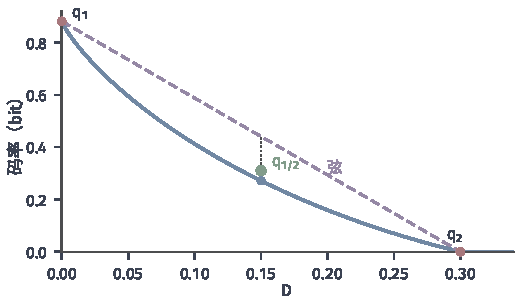
\includegraphics[width=88mm]{figures/07-probability/05-source-coding/matplotlib/rd-convexity/figure.pdf}
  \caption{$\operatorname{Bern}(0.3)$与Hamming失真下$R(D)$的凸性。红点$q_1$是照传（$D=0$，$I=h_2(0.3)$），$q_2$是恒输出$0$（$D=0.3$，$I=0$），紫色虚线是两者之间的弦，也是分时所能达到的点。绿点是两个测试信道各占一半的混合，高$0.3098$，蓝点是同一失真$0.15$下的$R(0.15)\approx0.2715$。}
  \label{fig:rd-convexity}
\end{BookInlineFigure}

\subsection{可行范围与零码率失真}
\label{sec:rd-feasible-range}

$R(D)$在哪些$D$上有限，在哪里降到零？下确界能否取到？这些问题决定了曲线的两个端点，也为编码定理的证明提供需要的连续性。本小节先设$\mathcal{X}$与$\hat{\mathcal{X}}$有限，$d$取非负有限值。

\paragraph{最小可行失真}
任何测试信道的平均失真都不会低于“每个源值都用它最好的重构”时的失真。对每个$x$，$d(x,\cdot)$按$q(\cdot\mid x)$的平均不小于它的最小值，再按$p(x)$平均得到$\mathbb{E}d\geq D_{\min}$，其中
\begin{equation}
  D_{\min}=\sum_{x}p(x)\min_{\hat{x}}d(x,\hat{x}).
  \label{eq:rd-dmin}
\end{equation}
把每个$x$确定地送到一个使$d(x,\cdot)$最小的$\hat{x}$，就达到$D_{\min}$。所以$D<D_{\min}$时可行集合为空，$R(D)=+\infty$；$D\geq D_{\min}$时可行集合非空。

另一端，若$\hat{X}$与$X$独立，平均失真是对重构边缘$r$的加权平均：
\[
  \mathbb{E}d=\sum_{\hat{x}}r(\hat{x})\sum_{x}p(x)d(x,\hat{x})\geq\min_{\hat{x}}\sum_{x}p(x)d(x,\hat{x}).
\]
右端记为
\begin{equation}
  D_{\max}=\min_{\hat{x}\in\hat{\mathcal{X}}}\sum_{x}p(x)\,d(x,\hat{x}),
  \label{eq:rd-dmax}
\end{equation}
它是只输出一个最佳常量时的失真，称为\term{零码率失真}（zero-rate distortion）。只输出一个常量不需要任何描述，所以$D\geq D_{\max}$时$R(D)=0$。

\begin{theorem}[最优测试信道的存在与$R$的连续性]
\label{thm:rd-existence}
设$\mathcal{X},\hat{\mathcal{X}}$有限，$d$非负有限。对每个$D\geq D_{\min}$，式~\eqref{eq:rd-information-rd}中的下确界可以取到，并且$R(D)\leq H(X)$。$R$在$[D_{\min},\infty)$上连续。
\end{theorem}

\begin{proof}
把测试信道看成$\mathbb{R}^{\lvert\mathcal{X}\rvert\times\lvert\hat{\mathcal{X}}\rvert}$中的矩阵。各行非负且和为$1$的矩阵组成有界闭集，式~\eqref{eq:rd-test-distortion}对$q$线性，$\mathbb{E}d\leq D$是一个闭的半空间。两者之交$\mathcal{Q}(D)$是非空紧集。

互信息对$q$连续。把式~\eqref{eq:rd-test-information}中的对数拆开，并按式~\eqref{eq:rd-output-marginal}合并$\hat{x}$相同的项，得
\[
  I(P_X,q)=\sum_{x,\hat{x}}p(x)\,\phi\bigl(q(\hat{x}\mid x)\bigr)-\sum_{\hat{x}}\phi\bigl(r_q(\hat{x})\bigr),
\]
其中$\phi(t)=t\log_2t$在$[0,1]$上连续，$r_q$对$q$线性。连续函数在非空紧集上取到最小值，所以下确界可以取到。又$I(P_X,q)\leq H(X)$对一切$q$成立，因为$I=H(X)-H(X\mid\hat{X})$，故$R(D)\leq H(X)$。

连续性先看内部。$R$在$[D_{\min},\infty)$上取有限值并且是凸函数，开区间上的凸函数连续，所以$R$在$(D_{\min},\infty)$上连续。

在端点$D_{\min}$处，取$D_k\downarrow D_{\min}$与相应的最优测试信道$q_k\in\mathcal{Q}(D_k)$。所有$q_k$落在紧集$\mathcal{Q}(D_1)$中，取收敛子列$q_{k_j}\to q$。由失真的线性与连续性，$q$的平均失真不超过$D_{\min}$，于是
\[
  R(D_{\min})\leq I(P_X,q)=\lim_{j\to\infty}R(D_{k_j}).
\]
另一方面$R$非增，$R(D_{k_j})\leq R(D_{\min})$。两边夹住，$R(D_k)\to R(D_{\min})$。
\end{proof}

\begin{theorem}[零码率失真]
\label{thm:rd-zero-rate}
在定理~\ref{thm:rd-existence}的条件下，$R(D)=0$当且仅当$D\geq D_{\max}$。在$[D_{\min},D_{\max}]$上$R$严格递减。
\end{theorem}

\begin{proof}
$D\geq D_{\max}$时恒输出最佳常量可行，互信息为零。反之设$R(D)=0$，由定理~\ref{thm:rd-existence}，存在可行的$q$使$I(P_X,q)=0$，即$X$与$\hat{X}$独立。由式~\eqref{eq:rd-dmax}前的计算，它的平均失真至少为$D_{\max}$，所以$D\geq D_{\max}$。

严格递减用反证。设$D_{\min}\leq D_1<D_2\leq D_{\max}$且$R(D_1)=R(D_2)$。由刚证明的结论，$D_1<D_{\max}$蕴含$R(D_1)>0$。若$D_2<D_{\max}$，把$D_2$写成$D_1$与$D_{\max}$的凸组合$D_2=\lambda D_1+(1-\lambda)D_{\max}$，$\lambda\in(0,1)$，由式~\eqref{eq:rd-convex}，
\[
  R(D_2)\leq\lambda R(D_1)+(1-\lambda)\cdot0<R(D_1),
\]
其中最后一步用了$R(D_1)>0$，与假设矛盾。若$D_2=D_{\max}$，则$R(D_1)=0$，与$D_1<D_{\max}$矛盾。
\end{proof}

当$\mathcal{X}=\hat{\mathcal{X}}$且$d(x,\hat{x})=0$当且仅当$x=\hat{x}$时，$D_{\min}=0$，而$\mathbb{E}d=0$迫使$\hat{X}=X$，于是$R(0)=I(X;X)=H(X)$。零失真的码率回到第~\ref{chap:lossless-coding}章的熵。雨天记录的例子中$D_{\min}=0$，$R(0)=h_2(0.3)$；零码率失真$D_{\max}=\min\{0.3,0.7\}=0.3$，就是一律猜“不下雨”。

\paragraph{一个$D_{\min}>0$的例子}
设$X$在$\{0,1,2\}$上取值，概率为$(0.3,0.4,0.3)$，而重构只能取$\hat{\mathcal{X}}=\{0,2\}$，失真为平方误差。$x=1$离两个重构值都是$1$，所以由式~\eqref{eq:rd-dmin}，
\[
  D_{\min}=0.4\times1=0.4 .
\]
两个常量重构的平均失真都是$0.4\times1+0.3\times4=1.6$，所以$D_{\max}=1.6$。

$D=D_{\min}$时，$0$必须重构为$0$，$2$必须重构为$2$，否则会多出$4$的失真；只有$x=1$可以自由选择。设它以概率$a$重构为$2$，则$\mathbb{P}(\hat{X}=2)=0.3+0.4a$，$H(\hat{X}\mid X)=0.4\,h_2(a)$，
\[
  I(a)=h_2(0.3+0.4a)-0.4\,h_2(a).
\]

用$h_2'(t)=\log_2\frac{1-t}{t}$求导，
\[
  I'(a)=0.4\log_2\frac{0.7-0.4a}{0.3+0.4a}-0.4\log_2\frac{1-a}{a}.
\]
令其为零，得$a(0.7-0.4a)=(1-a)(0.3+0.4a)$，展开后$0.7a=0.3+0.1a$，即$a=\tfrac12$。$I$是测试信道的凸函数，在这条线段上也凸，所以这是最小点：
\[
  R(D_{\min})=I\Bigl(\frac12\Bigr)=h_2(0.5)-0.4=0.6 .
\]
对照$a=0$时的$h_2(0.3)\approx0.881$与源熵$H(X)\approx1.571$：零失真不可行，在最小失真处也不必把源描述得一清二楚，那个处在中间、怎样重构都一样差的符号正好用来“抛硬币”。

图~\ref{fig:rd-ternary-range}画出这个例子的整条曲线。左侧浅红区域不可行；曲线从$(0.4,0.6)$开始，严格下降，在$D_{\max}=1.6$处降到零，之后保持为零。

\begin{BookInlineFigure}
  \centering
  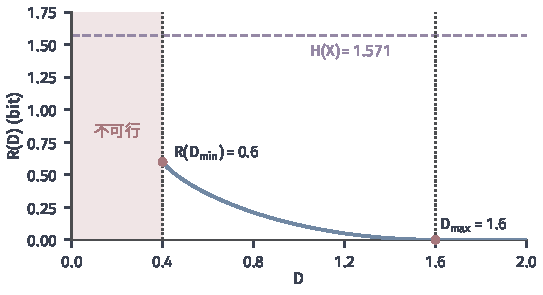
\includegraphics[width=92mm]{figures/07-probability/05-source-coding/matplotlib/rd-ternary-range/figure.pdf}
  \caption{三元信源$p=(0.3,0.4,0.3)$、重构字母表$\{0,2\}$与平方失真的$R(D)$（蓝线），由第~\ref{sec:rd-computation}节的算法逐点计算。浅红区域$D<D_{\min}=0.4$不可行；红点是$(D_{\min},0.6)$与$(D_{\max},0)$；紫色虚线是源熵$H(X)\approx1.571$\,bit。}
  \label{fig:rd-ternary-range}
\end{BookInlineFigure}

\paragraph{一般重构空间}
重构值取实数或其他无限集合时，上面每一步都要重新核对。$d$需要对乘积$\sigma$代数可测，平均失真才有定义；可行的Markov核要组成某种意义下的紧集，互信息要对这种收敛下半连续，下确界才能取到。这些条件并不自动成立。

设$X\sim\operatorname{Bern}(\tfrac12)$，重构只能取开区间$(0,1)$中的值，$d(x,\hat{x})=\lvert x-\hat{x}\rvert$。把式~\eqref{eq:rd-dmin}中的最小值换成下确界，$D_{\min}$仍是$0$，但没有重构值能让失真为零，平均失真为$0$的测试信道不存在，$R(0)=+\infty$。

另一方面，对任意$\varepsilon\in(0,\tfrac12)$，把$0$重构为$\varepsilon$、把$1$重构为$1-\varepsilon$，平均失真为$\varepsilon$，互信息为$1$。所以$R(D)\leq1$对一切$D>0$成立，$R$在$0$处从有限值跳到$+\infty$。这里$\hat{\mathcal{X}}$不紧，下确界“存在”只是一个数，最优重构并未取到，定理~\ref{thm:rd-existence}的结论也随之失效。


\section{率失真编码定理}
\label{sec:rd-coding-theorem}

现在有两个函数：$R_{\mathrm{op}}(D)$由所有块编码决定，$R(D)$由单个符号上的优化决定。本节证明它们相等。证明分两半：任何码的码率都不能低于$R(D)$，这是下界；存在一列码以任意接近$R(D)$的码率达到失真$D$，这是可达性。

本节的设定是：$\mathcal{X}$与$\hat{\mathcal{X}}$有限，信源无记忆，失真按式~\eqref{eq:rd-block-distortion}可分，并且$d_{\max}=\max_{x,\hat{x}}d(x,\hat{x})<\infty$（有限字母表上这自动成立）。由于每个符号的失真都不低于它的最佳重构，任何码都满足$\mathbb{E}d_n\geq D_{\min}$，所以$D<D_{\min}$时没有可达对，只需讨论$D\geq D_{\min}$。

\begin{theorem}[率失真编码定理]
\label{thm:rd-coding}
在上述设定下，对每个$D\geq D_{\min}$，
\begin{equation}
  R_{\mathrm{op}}(D)=R(D).
  \label{eq:rd-coding-theorem}
\end{equation}
\end{theorem}

定理只说极限。它不告诉我们给定块长$n$时最好的码有多好，也不给出能在合理时间内运行的编码器；这两点在本节末尾再谈。

\subsection{码率的下界}
\label{sec:rd-converse}

任取一个$(n,M)$码，记编号为$J=f_n(X^{n})$，重构为$\hat{X}^{n}=g_n(J)$，期望失真为$\Delta=\mathbb{E}d_n(X^{n},\hat{X}^{n})$。目标是证明
\begin{equation}
  \frac{\log_2M}{n}\geq R(\Delta).
  \label{eq:rd-converse}
\end{equation}
思路是图~\ref{fig:rd-converse-chain}：所有源符号都挤过一个只有$M$个值的编号；把每一对$(X_i,\hat{X}_i)$单独拿出来，得到$n$个单符号测试信道；它们的平均又是一个测试信道，失真恰好是$\Delta$。

\begin{BookInlineFigure}
  \centering
  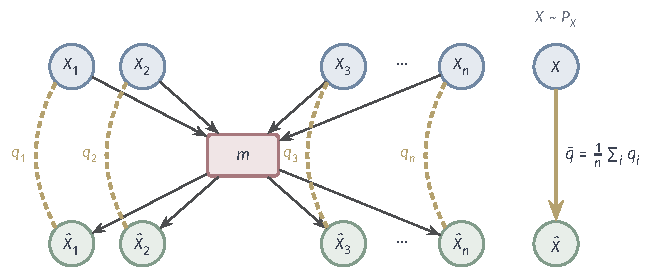
\includegraphics[width=110mm]{figures/07-probability/05-source-coding/tikz/rd-converse-chain/figure.pdf}
  \caption{下界证明的结构。蓝色源符号全部经过红框中的编号$J$（至多$M_n$个值）才到达绿色重构。黄色虚线表示每一对$(X_i,\hat{X}_i)$的条件分布，它是一个单符号测试信道$q_i$；右侧是它们的平均$\bar{q}$，输入仍服从$P_X$。}
  \label{fig:rd-converse-chain}
\end{BookInlineFigure}

\paragraph{第一步：编号限制信息}
$X^{n}\to J\to\hat{X}^{n}$构成Markov链：$\hat{X}^{n}$是$J$的函数，给定$J$后不再依赖$X^{n}$。由第~\ref{chap:information-measures}章的数据处理不等式，后处理不增加信息，
\[
  I(X^{n};\hat{X}^{n})\leq I(X^{n};J)\leq H(J)\leq\log_2M .
\]
第二个不等号是$I(X^{n};J)=H(J)-H(J\mid X^{n})$与条件熵非负，第三个是$J$只取$M$个值。

\paragraph{第二步：拆成单个符号}
把互信息写成源块的熵减去给定重构后的条件熵。信源无记忆，各$X_i$独立，联合熵可加：
\[
  H(X^{n})=\sum_{i=1}^{n}H(X_i).
\]
条件熵用链式法则逐个展开，再用“条件越多熵越小”去掉多余的条件：
\[
  H(X^{n}\mid\hat{X}^{n})=\sum_{i=1}^{n}H(X_i\mid X_1,\dots,X_{i-1},\hat{X}^{n})\leq\sum_{i=1}^{n}H(X_i\mid\hat{X}_i).
\]
两式相减，得到
\[
  I(X^{n};\hat{X}^{n})\geq\sum_{i=1}^{n}\bigl(H(X_i)-H(X_i\mid\hat{X}_i)\bigr)=\sum_{i=1}^{n}I(X_i;\hat{X}_i).
\]

\paragraph{第三步：平均成一个测试信道}
记第$i$个位置的条件分布为
\[
  q_i(\hat{x}\mid x)=\mathbb{P}(\hat{X}_i=\hat{x}\mid X_i=x),
\]
对$p(x)>0$的$x$定义，其余$x$任取一个分布。因为每个$X_i$都服从$P_X$，第$i$对的互信息就是$I(P_X,q_i)$。第$i$个位置的平均失真记为$\Delta_i$，它就是$q_i$在式~\eqref{eq:rd-test-distortion}中的失真。

令$\bar{q}=\frac1n\sum_iq_i$，由引理~\ref{lem:rd-mi-convex}（推广到$n$个信道的凸组合，按$n$归纳），
\[
  \frac1n\sum_{i=1}^{n}I(P_X,q_i)\geq I(P_X,\bar{q}).
\]
失真对测试信道线性，$\bar{q}$的平均失真是$\frac1n\sum_i\Delta_i$。由式~\eqref{eq:rd-block-distortion}，它正是$\Delta$。所以$\bar{q}$在$R(\Delta)$的可行集合中，$I(P_X,\bar{q})\geq R(\Delta)$。

把三步连起来：
\[
  \log_2M\geq I(X^{n};\hat{X}^{n})\geq\sum_{i=1}^{n}I(P_X,q_i)\geq n\,I(P_X,\bar{q})\geq n\,R(\Delta),
\]
这就是式~\eqref{eq:rd-converse}。

\paragraph{从单个码到渐近下界}
设$(R',D)$可达，相应码列的期望失真为$\Delta_n$，$\limsup_n\Delta_n\leq D$。对任意$\varepsilon>0$，$n$充分大时$\Delta_n\leq D+\varepsilon$，由式~\eqref{eq:rd-converse}与$R$非增，
\[
  \frac{\log_2M_n}{n}\geq R(\Delta_n)\geq R(D+\varepsilon).
\]
取上极限得$R'\geq R(D+\varepsilon)$。由定理~\ref{thm:rd-existence}，$R$在$[D_{\min},\infty)$上连续，令$\varepsilon\to0$得$R'\geq R(D)$。所以$R_{\mathrm{op}}(D)\geq R(D)$。

\paragraph{两个假设各用在哪里}
无记忆性用在第二步与第三步：$H(X^{n})=\sum_iH(X_i)$需要独立，$I(X_i;\hat{X}_i)=I(P_X,q_i)$需要每个$X_i$的分布都是$P_X$。可分失真用在第三步的最后：$\bar{q}$的失真等于块失真，靠的是块失真等于逐符号失真的平均。

去掉无记忆性，单符号的$R(D)$就不再是正确答案。设$Y\sim\operatorname{Bern}(0.3)$，令$X_1=X_2=\dots=X_n=Y$。每个$X_i$的分布仍是$\operatorname{Bern}(0.3)$，单符号的$R(0)$仍是$h_2(0.3)\approx0.881$。可是整块只有两种可能，用$1$\,bit传送$Y$就能零失真重构，码率$1/n\to0$。第二步中
\[
  H(X^{n})=h_2(0.3),\qquad \sum_{i=1}^{n}H(X_i)=n\,h_2(0.3),
\]
前者远小于后者，链条在这里断开。带记忆的信源需要按块定义信息量再取极限，本章不讨论。

\subsection{可达的码率}
\label{sec:rd-achievability}

下界说码率不能低于$R(D)$。反方向要构造码。直接设计最优码本很难，下面的办法是随机撒点：按最优测试信道的重构边缘独立地生成很多码字，证明平均而言总有一个码字离源块足够近，再由平均推出确定的好码本存在。

\paragraph{为什么随机码本能覆盖}
取达到$R(D)$的测试信道$q$（定理~\ref{thm:rd-existence}保证存在），它的重构边缘为$r=r_q$，$I=I(P_X,q)=R(D)$。对一个典型的源块$x^{n}$，随机抽一个码字$Y^{n}$，各分量独立服从$r$，它“恰好与$x^{n}$配成像是由$q$产生的一对”的概率有多大？

对一对$(x,\hat{x})$，记\term{信息密度}（information density）
\begin{equation}
  \imath(x,\hat{x})=\log_2\frac{q(\hat{x}\mid x)}{r(\hat{x})},\qquad
  \imath_n(x^{n},\hat{x}^{n})=\sum_{i=1}^{n}\imath(x_i,\hat{x}_i),
  \label{eq:rd-information-density}
\end{equation}
只在$q(\hat{x}\mid x)>0$处定义。按联合分布$p(x)q(\hat{x}\mid x)$取期望，由式~\eqref{eq:rd-test-information}，$\mathbb{E}\,\imath(X,\hat{X})=I$。$\imath_n$越大，块对$(x^{n},\hat{x}^{n})$在$q$下比在“$\hat{x}^{n}$与$x^{n}$无关”时越可能出现，倍数是$2^{\imath_n}$。

若$(X_i,\hat{X}_i)$独立地按$p(x)q(\hat{x}\mid x)$产生，大数律使$\frac1n\imath_n$集中在$I$附近，图~\ref{fig:rd-info-density}展示了这种集中。于是“像是由$q$产生的”块对，其$\imath_n$约为$nI$，从$r^{n}$中独立抽到这样的$\hat{x}^{n}$的概率约为$2^{-nI}$。要有把握至少抽中一个，码字数应超过$2^{nI}$，也就是码率略高于$I=R(D)$。

\begin{BookInlineFigure}
  \centering
  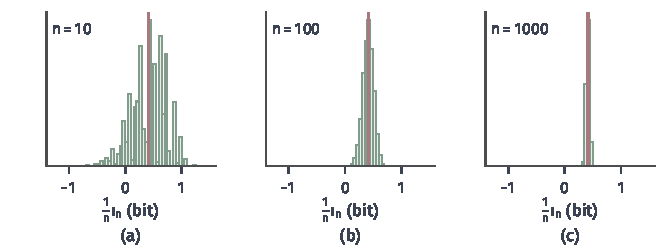
\includegraphics[width=112mm]{figures/07-probability/05-source-coding/matplotlib/rd-info-density/figure.pdf}
  \caption{$\operatorname{Bern}(0.3)$信源、Hamming失真、$D=0.1$的最优联合分布下，每符号信息密度$\frac1n\imath_n$的直方图（绿），块长$n=10,100,1000$，各$20000$个块，随机种子$722$。单个符号的$\imath$只取$0.363$、$-2.807$、$-1.585$、$1.585$四个值；红线是均值$I=R(0.1)\approx0.412$。$n=1000$时样本标准差约为$0.029$。}
  \label{fig:rd-info-density}
\end{BookInlineFigure}

下面把这个估计写成不等式。对$\gamma>0$与$D'\geq0$，令
\[
  \mathcal{A}=\Bigl\{(x^{n},\hat{x}^{n}):\ q^{n}(\hat{x}^{n}\mid x^{n})>0,\ \imath_n(x^{n},\hat{x}^{n})\leq\log_2\gamma,\ d_n(x^{n},\hat{x}^{n})\leq D'\Bigr\},
\]
其中$q^{n}$是$q$逐符号作用于整块的条件概率，即各分量$q(\hat{x}_i\mid x_i)$的乘积。$\mathcal{A}$中的块对失真达标，信息密度又不过大，称为\term{失真典型集}（distortion-typical set）。对固定的$x^{n}$，把与它配成$\mathcal{A}$中块对的重构块全体记为$\mathcal{A}(x^{n})$。

\begin{lemma}[随机码本的覆盖]
\label{lem:rd-covering}
设码字$C_1,\dots,C_M$相互独立，各分量独立服从$r$，并与$X^{n}$独立。令$(X^{n},\hat{X}^{n})$按$\prod_ip(x_i)q(\hat{x}_i\mid x_i)$分布。则
\begin{equation}
  \mathbb{P}\bigl(\text{没有}C_m\in\mathcal{A}(X^{n})\bigr)\leq\mathbb{P}\bigl((X^{n},\hat{X}^{n})\notin\mathcal{A}\bigr)+\mathrm{e}^{-M/\gamma}.
  \label{eq:rd-covering}
\end{equation}
\end{lemma}

\begin{proof}
固定$x^{n}$，令
\[
  g(x^{n})=\sum_{\hat{x}^{n}\in\mathcal{A}(x^{n})}q^{n}(\hat{x}^{n}\mid x^{n}),
\]
它是按测试信道重构时落入$\mathcal{A}(x^{n})$的概率。对$\hat{x}^{n}\in\mathcal{A}(x^{n})$，由式~\eqref{eq:rd-information-density}，
\[
  r^{n}(\hat{x}^{n})=q^{n}(\hat{x}^{n}\mid x^{n})\,2^{-\imath_n(x^{n},\hat{x}^{n})}\geq\frac{1}{\gamma}\,q^{n}(\hat{x}^{n}\mid x^{n}),
\]
其中$r^{n}(\hat{x}^{n})=\prod_ir(\hat{x}_i)$。对$\mathcal{A}(x^{n})$求和，单个码字落入$\mathcal{A}(x^{n})$的概率至少是$g(x^{n})/\gamma$。

$M$个码字独立，全部落空的概率是
\[
  \Bigl(1-\mathbb{P}\bigl(C_1\in\mathcal{A}(x^{n})\bigr)\Bigr)^{M}\leq\Bigl(1-\frac{g(x^{n})}{\gamma}\Bigr)^{M}\leq\exp\Bigl(-\frac{M\,g(x^{n})}{\gamma}\Bigr),
\]
最后一步用了$1-u\leq\mathrm{e}^{-u}$。

再把指数关于$g$放大成线性函数。对$c\geq0$，$t\mapsto\mathrm{e}^{-ct}$在$[0,1]$上凸，图像在两端点连线之下：
\[
  \mathrm{e}^{-ct}\leq(1-t)+t\,\mathrm{e}^{-c}\leq1-t+\mathrm{e}^{-c},\qquad t\in[0,1].
\]
取$c=M/\gamma$，$t=g(x^{n})$，全部落空的概率至多为$1-g(x^{n})+\mathrm{e}^{-M/\gamma}$。

最后对$x^{n}$按$P_X^{n}$平均。$1-g(X^{n})$的期望正是$(X^{n},\hat{X}^{n})\notin\mathcal{A}$的概率，于是得到式~\eqref{eq:rd-covering}。
\end{proof}

式~\eqref{eq:rd-covering}右端两项各有分工。第一项是测试信道本身“不典型”的概率，由大数律控制；第二项是码字太少、撒网不够密的代价，只要$M$远大于$\gamma\approx2^{nI}$就可忽略。

\begin{theorem}[可达性]
\label{thm:rd-achievability}
在本节设定下，对$D\geq D_{\min}$与任意$R'>R(D)$，$(R',D)$可达。于是$R_{\mathrm{op}}(D)\leq R(D)$。
\end{theorem}

\begin{proof}
取$\delta>0$，令$I=R(D)$，$q$为达到$R(D)$的测试信道，$\mathbb{E}_qd\leq D$。下面分四步。

\emph{码本大小。}令$\gamma_n=2^{n(I+\delta)}$，$M_n=\lceil2^{n(I+2\delta)}\rceil$，$D'=D+\delta$。码率满足
\[
  \frac{\log_2M_n}{n}\leq\frac{\log_2\bigl(2^{n(I+2\delta)}+1\bigr)}{n}\to I+2\delta .
\]

\emph{覆盖失败的概率。}$(X_i,\hat{X}_i)$独立同分布，$\imath(X_i,\hat{X}_i)$只取有限个值，均值为$I$；$d(X_i,\hat{X}_i)$有界，均值不超过$D$。由第~\ref{chap:laws-of-large-numbers}章的弱大数律，
\[
  \mathbb{P}\Bigl(\frac1n\imath_n>I+\delta\Bigr)\to0,\qquad \mathbb{P}\bigl(d_n>D+\delta\bigr)\to0 .
\]
所以式~\eqref{eq:rd-covering}的第一项趋于零。第二项中$M_n/\gamma_n\geq2^{n\delta}$，故
\[
  \mathrm{e}^{-M_n/\gamma_n}\leq\exp(-2^{n\delta})\to0 .
\]记右端为$\varepsilon_n$，$\varepsilon_n\to0$。

\emph{随机码的平均失真。}用最近码字编码器。只要有一个$C_m\in\mathcal{A}(X^{n})$，最近码字的失真就不超过$D+\delta$；否则失真不超过$d_{\max}$。对源与码本一起取期望，
\[
  \mathbb{E}\bigl[d_n(X^{n},\hat{X}^{n})\bigr]\leq D+\delta+d_{\max}\,\varepsilon_n .
\]

\emph{从随机码本到确定码本。}左端是对随机码本取平均后的期望失真，平均值不超过某个数，至少有一个码本的期望失真不超过这个数。于是对每个充分大的$n$，存在确定的$(n,M_n)$码，期望失真不超过$D+\delta+d_{\max}\varepsilon_n$。对较小的$n$随便取一个码，不影响上极限。这说明$(I+2\delta,D+\delta)$可达。

$\delta$可以任意小。给定$R'>I$，对一切满足$I+2\delta\leq R'$的$\delta$，$(R',D+\delta)$都可达。下面的对角线论证说明$(R',D)$也可达。
\end{proof}

\paragraph{边界点的极限处理}
设对每个$k$，$(R',D+\tfrac1k)$可达，相应的码列为$\mathcal{C}^{(k)}$。由上极限的定义，存在$N_k$，使$n\geq N_k$时$\mathcal{C}^{(k)}$中块长为$n$的码满足
\[
  \frac{\log_2M_n}{n}\leq R'+\frac1k,\qquad \mathbb{E}d_n\leq D+\frac2k .
\]
可以取$N_1<N_2<\cdots$。对$N_k\leq n<N_{k+1}$，块长$n$时使用$\mathcal{C}^{(k)}$中的码。$n\to\infty$时所用的$k$也趋于无穷，所以新码列满足式~\eqref{eq:rd-achievable}，$(R',D)$可达。可达区域在这个意义下是闭的。

至此$R_{\mathrm{op}}(D)\leq R(D)$，与第~\ref{sec:rd-converse}节的下界合起来，定理~\ref{thm:rd-coding}得证。在$D=D_{\min}$处，下界用到了$R$在端点的右连续，可达性则靠这里的极限处理；两边都不要求在端点处有特别的构造。

\paragraph{有限块长与计算代价}
定理只保证极限。先给极限一个记号：由定理~\ref{thm:rd-zero-rate}，$R$在$[D_{\min},D_{\max}]$上严格递减，它的反函数记为$D(R)$，称为\term{失真率函数}（distortion-rate function），表示码率为$R$时能达到的最小失真。雨天记录中$D(0.5)\approx0.0742$，即$R(D)=0.5$的解。

图~\ref{fig:rd-finite-codes}(a)用穷举给出$n\leq4$时每种码本大小下最好的码，它们都在曲线上方不远处，码率$\tfrac12$时最好的失真从$n=2$的$0.15$降到$n=4$的约$0.136$，离$D(0.5)$仍有距离。图~\ref{fig:rd-finite-codes}(b)是按证明构造的随机码本：码率固定为$\tfrac12$，块长到$36$时平均失真约为$0.097$，仍明显高于极限。

\begin{BookInlineFigure}
  \centering
  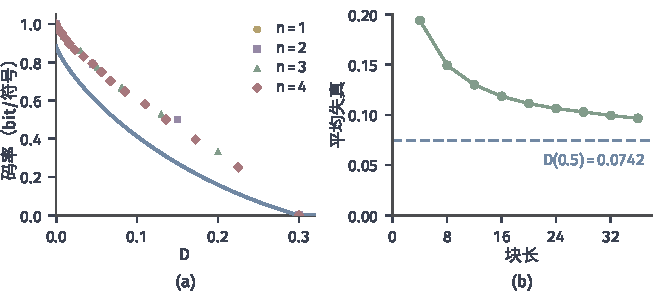
\includegraphics[width=112mm]{figures/07-probability/05-source-coding/matplotlib/rd-finite-codes/figure.pdf}
  \caption{$\operatorname{Bern}(0.3)$信源与Hamming失真下的有限块长码。(a)对$n=1,2,3,4$穷举全部码本，每种码本大小$M$下期望失真最小的码（不同颜色与形状），横坐标为失真，纵坐标为$\log_2M/n$；蓝线是$R(D)$。(b)码率$\tfrac12$的随机码本，码字各分量独立服从$\operatorname{Bern}(0.265)$（码率$\tfrac12$对应的最优重构边缘），最近码字编码；每个$n$用$40$个码本、每个码本$250$个源块估计平均失真，随机种子$722$。蓝色虚线是$D(0.5)\approx0.0742$。}
  \label{fig:rd-finite-codes}
\end{BookInlineFigure}

收敛慢的原因可以从证明中看出：$\frac1n\imath_n$与$d_n$的波动按$n^{-1/2}$缩小，要让它们都落在$\delta$以内，$n$要远大于$\delta^{-2}$。计算上，最近码字编码要在$2^{nR}$个码字中搜索，$n=36$、$R=\tfrac12$时已有约$2.6\times10^{5}$个码字。证明给出的是存在性，构造搜索代价低的好码是另一个问题，本章不讨论。


\section{可解析的模型}
\label{sec:rd-analytic}

编码定理把问题交还给式~\eqref{eq:rd-information-rd}的优化。少数模型可以精确求解，办法都是两步：先证明一个对所有满足失真约束的测试信道都成立的互信息下界，再构造一个测试信道使下界取等号。下界说“不可能更省”，构造说“确实能做到”，两者相遇处就是$R(D)$。

构造时常常反过来想：不直接写$q(\hat{x}\mid x)$，而是先给出$\hat{X}$的分布，再说明$X$怎样由$\hat{X}$加上一个独立的“误差”得到。这种从重构到源的描述称为\term{反向测试信道}（backward test channel）。只要它产生的$X$恰好服从给定的源分布，对$X$取条件就得到一个普通的测试信道。

\subsection{二元信源}
\label{sec:rd-binary}

开头的雨天记录现在可以算到底。设$X\sim\operatorname{Bern}(p)$，失真为Hamming失真。交换符号$0$与$1$不改变问题，所以不妨设$p\leq\tfrac12$。由第~\ref{sec:rd-feasible-range}节，$D_{\min}=0$，$D_{\max}=p$，零码率时一律输出更常见的$0$。

\begin{theorem}[二元信源的率失真函数]
\label{thm:rd-binary}
设$X\sim\operatorname{Bern}(p)$，$0\leq p\leq\tfrac12$，失真为式~\eqref{eq:rd-hamming}。则
\begin{equation}
  R(D)=\begin{cases}
    h_2(p)-h_2(D), & 0\leq D\leq p,\\
    0, & D\geq p.
  \end{cases}
  \label{eq:rd-binary}
\end{equation}
\end{theorem}

\begin{proof}
$D\geq p$时由定理~\ref{thm:rd-zero-rate}得$R(D)=0$。下面设$0\leq D<p$，于是$p>0$。

\emph{下界。}任取满足$\mathbb{E}d\leq D$的测试信道，令$E=X\oplus\hat{X}$为模$2$和，$E=1$表示重构出错，$\mathbb{P}(E=1)=\mathbb{E}d\leq D$。给定$\hat{X}$时，$X\mapsto X\oplus\hat{X}$是一一对应，条件熵不变，所以
\[
  H(X\mid\hat{X})=H(E\mid\hat{X})\leq H(E)=h_2\bigl(\mathbb{P}(E=1)\bigr)\leq h_2(D).
\]
最后一步用了$h_2$在$[0,\tfrac12]$上递增，以及$\mathbb{P}(E=1)\leq D<\tfrac12$。于是
\[
  I(X;\hat{X})=H(X)-H(X\mid\hat{X})\geq h_2(p)-h_2(D).
\]

\emph{达到下界。}令
\[
  r=\frac{p-D}{1-2D}.
\]
由$0\leq D<p\leq\tfrac12$，分子与分母都为正；又$p\leq\tfrac12<1-D$，所以$p-D<1-2D$，$r\in(0,1)$。取相互独立的$\hat{X}\sim\operatorname{Bern}(r)$与$Z\sim\operatorname{Bern}(D)$，令$X=\hat{X}\oplus Z$。

$X=1$当且仅当$\hat{X}$与$Z$恰有一个为$1$，
\[
  \mathbb{P}(X=1)=r(1-D)+(1-r)D=D+r(1-2D)=p ,
\]
所以$X$恰好服从源分布，$(X,\hat{X})$的联合分布给出一个测试信道。它的失真是$\mathbb{P}(X\neq\hat{X})=\mathbb{P}(Z=1)=D$。$Z$与$\hat{X}$独立，
\[
  I(X;\hat{X})=H(X)-H(X\mid\hat{X})=h_2(p)-H(Z\mid\hat{X})=h_2(p)-h_2(D),
\]
与下界相等。
\end{proof}

下界的证明说明了等号何时成立：错误指示$E$必须与$\hat{X}$独立，并且错误率恰为$D$。构造的反向测试信道正好满足这两点。图~\ref{fig:rd-binary-test-channels}(a)画出$p=0.3$、$D=0.1$时的反向信道：$\hat{X}\sim\operatorname{Bern}(0.25)$，再以$0.1$的概率翻转，得到$\operatorname{Bern}(0.3)$。

用Bayes公式换回从$X$到$\hat{X}$的方向。$X=0$而$\hat{X}=1$需要$\hat{X}=1$且$Z=1$；$X=1$而$\hat{X}=0$需要$\hat{X}=0$且$Z=1$。于是
\[
  \begin{aligned}
  q(1\mid0)&=\frac{rD}{1-p}=\frac{0.25\times0.1}{0.7}=\frac1{28},\\
  q(0\mid1)&=\frac{(1-r)D}{p}=\frac{0.75\times0.1}{0.3}=\frac14 ,
  \end{aligned}
\]
这就是第~\ref{sec:rd-test-channels}节第三个测试信道，图~\ref{fig:rd-binary-test-channels}(b)画出了它。由式~\eqref{eq:rd-binary}，
\[
  R(0.1)=h_2(0.3)-h_2(0.1)\approx0.8813-0.4690=0.4123 .
\]

\begin{BookInlineFigure}
  \centering
  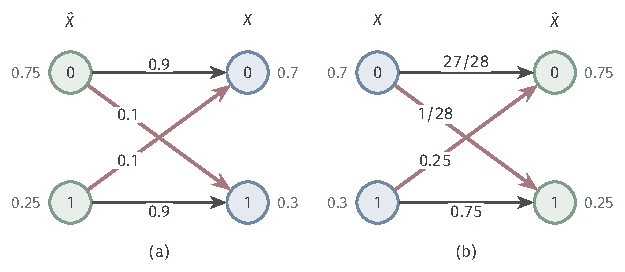
\includegraphics[width=106mm]{figures/07-probability/05-source-coding/tikz/rd-binary-test-channels/figure.pdf}
  \caption{$X\sim\operatorname{Bern}(0.3)$、Hamming失真、$D=0.1$的最优测试信道。(a)反向形式：绿色的$\hat{X}\sim\operatorname{Bern}(0.25)$经过独立的翻转（红箭头，概率$0.1$）得到蓝色的$X$，节点旁的数是边缘概率。(b)由Bayes公式得到的正向形式$q(\hat{x}\mid x)$，罕见符号$1$被改错的概率$\tfrac14$远大于常见符号$0$的$\tfrac1{28}$。}
  \label{fig:rd-binary-test-channels}
\end{BookInlineFigure}

开头的问题有了答案：允许错$10\%$，每天只需约$0.412$\,bit，不到无损所需$0.881$\,bit的一半，远少于按比例打折的$0.881\times0.9\approx0.793$。第~\ref{sec:rd-block-model}节中要求每一块都不超过$10\%$错误时至少需要$0.531$\,bit；期望失真要求允许少数块错得多，于是更省。

\paragraph{源概率与端点}
图~\ref{fig:rd-binary-curves}画出三个源概率下的曲线，可以对照式~\eqref{eq:rd-binary}逐项检查。
\begin{itemize}
  \item $D=0$时$R(0)=h_2(p)=H(X)$，回到无损编码的熵。
  \item 曲线在$D_{\max}=p$处降到零，零码率失真由源概率决定：$p=0.1$时一律猜$0$只错$10\%$，$p=\tfrac12$时要错一半。
  \item 均匀信源$p=\tfrac12$时$R(D)=1-h_2(D)$，这只是$p$的一个取值，曲线最高，因为每个符号最难预测。
  \item 退化情形$p=0$时信源是常数$0$，$D_{\max}=0$，$R\equiv0$；这时$h_2(p)-h_2(D)$在$D>0$时为负，公式只能在$0\leq D\leq p$上使用。
\end{itemize}

曲线的斜率是$R'(D)=-h_2'(D)=-\log_2\frac{1-D}{D}$，$D\downarrow0$时趋于$-\infty$。允许极少量的错误就能省下相当多的码率，这是有损压缩在低失真端最划算的原因；越往后，每多容忍一点失真省下的码率越少。

\begin{BookInlineFigure}
  \centering
  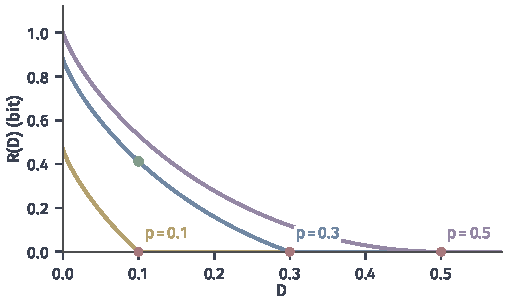
\includegraphics[width=86mm]{figures/07-probability/05-source-coding/matplotlib/rd-binary-curves/figure.pdf}
  \caption{$\operatorname{Bern}(p)$信源在Hamming失真下的$R(D)$，$p=0.1$（黄）、$0.3$（蓝）、$0.5$（紫）。红点是零码率失真$D_{\max}=p$，曲线在纵轴上的截距是$h_2(p)$。绿点是贯穿例子$(0.1,0.4123)$。}
  \label{fig:rd-binary-curves}
\end{BookInlineFigure}

\subsection{高斯信源}
\label{sec:rd-gaussian}

开头的第二个问题涉及实值信源与平方失真。这里重构值连续变化，第~\ref{sec:rd-coding-theorem}节的有限字母表证明不能直接搬用；我们先在信息率失真函数的层面上求解，再说明编码定理在这里的地位。计算需要一个关于微分熵的不等式，它也会在第~\ref{chap:gaussian-channel-capacity}章计算高斯信道容量时用到。

本小节沿用第~\ref{chap:information-measures}章的微分熵，换成以bit计：对有密度$f$的实值随机变量，
\[
  h(X)=-\int_{\mathbb{R}}f(x)\log_2f(x)\,\mathrm{d}x ,
\]
前提是这个积分有意义。KL散度同样以bit计，即在第~\ref{chap:distribution-comparison}章的定义中把$\ln$换成$\log_2$，它仍然非负，且为零当且仅当两个分布相同。

\subsubsection{高斯分布的熵上界}
\label{sec:rd-gaussian-entropy}

方差固定时，哪种分布的不确定性最大？图~\ref{fig:rd-gaussian-entropy}中三个密度均值都是$0$、方差都是$1$。均匀分布把质量平铺在$[-\sqrt3,\sqrt3]$上，Laplace分布尖峰更高、尾部更厚，高斯分布介于两者之间。它们的微分熵分别是
\[
  \log_2(2\sqrt3)\approx1.792,\qquad \log_2(\sqrt2\,\mathrm{e})\approx1.943,\qquad \frac12\log_2(2\pi\mathrm{e})\approx2.047 ,
\]
第二个用了Laplace分布$\operatorname{Laplace}(0,b)$的方差$2b^{2}=1$与熵$\log_2(2\mathrm{e}b)$。高斯最大，这不是巧合。

\begin{BookInlineFigure}
  \centering
  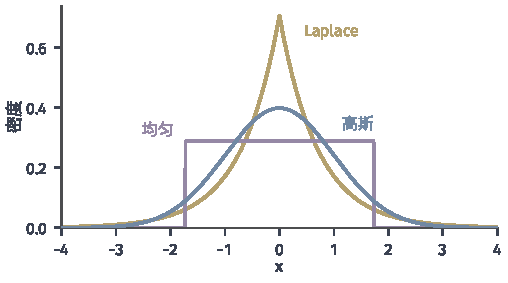
\includegraphics[width=86mm]{figures/07-probability/05-source-coding/matplotlib/rd-gaussian-entropy/figure.pdf}
  \caption{均值为$0$、方差为$1$的三个密度：标准高斯（蓝，$h\approx2.047$\,bit）、$\operatorname{Laplace}(0,1/\sqrt2)$（黄，$h\approx1.943$\,bit）、$[-\sqrt3,\sqrt3]$上的均匀分布（紫，$h\approx1.792$\,bit）。三个熵值也用数值积分核对过。}
  \label{fig:rd-gaussian-entropy}
\end{BookInlineFigure}

\begin{theorem}[固定方差的熵上界]
\label{thm:rd-gaussian-max-entropy}
设实值随机变量$X$有密度$f$，均值为$\mu$，方差$\sigma^{2}\in(0,\infty)$。则定义$h(X)$的积分有意义，取值于$[-\infty,\infty)$，并且
\begin{equation}
  h(X)\leq\frac12\log_2(2\pi\mathrm{e}\sigma^{2}),
  \label{eq:rd-gaussian-max-entropy}
\end{equation}
等号成立当且仅当$X\sim\mathcal{N}(\mu,\sigma^{2})$。
\end{theorem}

\begin{proof}
取同均值、同方差的高斯密度作参考，
\[
  g(x)=\frac{1}{\sqrt{2\pi\sigma^{2}}}\exp\Bigl(-\frac{(x-\mu)^{2}}{2\sigma^{2}}\Bigr).
\]
先算$-\log_2g$在$f$下的期望。由$g$的表达式，
\[
  -\log_2g(x)=\frac12\log_2(2\pi\sigma^{2})+(\log_2\mathrm{e})\frac{(x-\mu)^{2}}{2\sigma^{2}},
\]
它是$x$的二次函数，在$f$下可积。由$\mathbb{E}(X-\mu)^{2}=\sigma^{2}$，
\[
  -\int f\log_2g\,\mathrm{d}x=\frac12\log_2(2\pi\sigma^{2})+\frac{\log_2\mathrm{e}}{2}=\frac12\log_2(2\pi\mathrm{e}\sigma^{2}).
\]

再看KL散度的被积函数$f\log_2(f/g)$（在$f>0$处）。由$\ln t\geq1-1/t$，
\[
  f\ln\frac{f}{g}\geq f-g ,
\]
所以它的负部不超过$g$，可积。于是KL散度
\[
  D_{\mathrm{KL}}(f\Vert g)=\int f\log_2\frac{f}{g}\,\mathrm{d}x
\]
有意义，取值于$[0,\infty]$。

在$f>0$处写$f\log_2f=f\log_2(f/g)+f\log_2g$。右端第一项负部可积，第二项可积，所以$f\log_2f$的负部可积，$\int f\log_2f\,\mathrm{d}x$有意义且大于$-\infty$。这说明$h(X)$有意义，取值于$[-\infty,\infty)$，并且
\[
  h(X)=-\int f\log_2\frac{f}{g}\,\mathrm{d}x-\int f\log_2g\,\mathrm{d}x=\frac12\log_2(2\pi\mathrm{e}\sigma^{2})-D_{\mathrm{KL}}(f\Vert g).
\]
KL散度非负，得到式~\eqref{eq:rd-gaussian-max-entropy}。等号成立当且仅当$D_{\mathrm{KL}}(f\Vert g)=0$，即$f=g$几乎处处，也就是$X\sim\mathcal{N}(\mu,\sigma^{2})$。
\end{proof}

证明里的关键是：$-\log_2g$只是$x$的二次函数，它在任何同方差分布下的平均都一样。于是“$f$的熵比高斯少多少”恰好就是$f$与高斯的KL散度。条件中的方差有限保证了这个平均有限；$h(X)$可以是$-\infty$（例如密度在某些点附近极度集中），不等式仍然成立，只是没有信息量。没有方差限制时，微分熵没有上界：$\operatorname{Unif}(0,a)$的熵$\log_2a$随$a$无限增大。

\subsubsection{高斯率失真函数}
\label{sec:rd-gaussian-rd}

设$X\sim\mathcal{N}(\mu,\sigma^{2})$，$\sigma^{2}>0$，失真为平方误差。测试信道是从$\mathbb{R}$到$\mathbb{R}$的Markov核，$R(D)$仍按式~\eqref{eq:rd-information-rd}定义，互信息是联合分布相对边缘乘积的KL散度，可以为$+\infty$。

\begin{theorem}[高斯信源的率失真函数]
\label{thm:rd-gaussian}
在上述设定下，
\begin{equation}
  R(D)=\begin{cases}
    \dfrac12\log_2\dfrac{\sigma^{2}}{D}, & 0<D<\sigma^{2},\\
    0, & D\geq\sigma^{2},
  \end{cases}
  \label{eq:rd-gaussian}
\end{equation}
且$R(0)=+\infty$。单位是bit每个实值源符号。
\end{theorem}

\begin{proof}
把$X$与$\hat{X}$同时减去$\mu$，平方误差与互信息都不变，所以不妨设$\mu=0$。$D\geq\sigma^{2}$时恒输出$0$，失真为$\mathbb{E}X^{2}=\sigma^{2}\leq D$，互信息为零。下面设$0<D<\sigma^{2}$，分下界与达到两部分。

\emph{下界的分解。}任取满足$\mathbb{E}(X-\hat{X})^{2}\leq D$的联合分布。若$I(X;\hat{X})=+\infty$无需证明，下设它有限。这时联合分布对$P_X\otimes P_{\hat{X}}$绝对连续，记Radon–Nikodym导数为$\lambda(x,\hat{x})$，则互信息是$\log_2\lambda(X,\hat{X})$的期望。$P_X$有密度$f=\varphi_{\sigma^{2}}$（方差为$\sigma^{2}$的零均值高斯密度），所以给定$\hat{X}=\hat{x}$时$X$的条件分布有密度$p(x\mid\hat{x})=\lambda(x,\hat{x})f(x)$，并且
\[
  I(X;\hat{X})=\mathbb{E}\Bigl[\log_2\frac{p(X\mid\hat{X})}{f(X)}\Bigr].
\]

\emph{条件高斯参考。}引入一个“猜测”的条件密度$w(x\mid\hat{x})=\varphi_D(x-\hat{x})$，即以$\hat{x}$为中心、方差为$D$的高斯密度。把对数拆成两项：
\[
  \log_2\frac{p(X\mid\hat{X})}{f(X)}=\log_2\frac{p(X\mid\hat{X})}{w(X\mid\hat{X})}+\log_2\frac{w(X\mid\hat{X})}{f(X)} .
\]
第二项写开是
\[
  \frac12\log_2\frac{\sigma^{2}}{D}-\frac{\log_2\mathrm{e}}{2}\Bigl(\frac{(X-\hat{X})^{2}}{D}-\frac{X^{2}}{\sigma^{2}}\Bigr),
\]
由$\mathbb{E}X^{2}=\sigma^{2}$与$\mathbb{E}(X-\hat{X})^{2}\leq D$，它可积，期望至少为
\[
  \frac12\log_2\frac{\sigma^{2}}{D}-\frac{\log_2\mathrm{e}}{2}\,(1-1)=\frac12\log_2\frac{\sigma^{2}}{D}.
\]

\emph{条件KL非负。}左端与第二项都可积，所以第一项可积。对$\hat{X}$取条件，第一项的条件期望是条件分布$p(\cdot\mid\hat{X})$相对参考$w(\cdot\mid\hat{X})$的KL散度，非负；再对$\hat{X}$平均仍非负。于是
\[
  I(X;\hat{X})\geq\frac12\log_2\frac{\sigma^{2}}{D}.
\]

\emph{达到下界。}取相互独立的$\hat{X}\sim\mathcal{N}(0,\sigma^{2}-D)$与$Z\sim\mathcal{N}(0,D)$，令$X=\hat{X}+Z$。独立高斯之和仍是高斯，$X\sim\mathcal{N}(0,\sigma^{2})$，失真$\mathbb{E}(X-\hat{X})^{2}=\mathbb{E}Z^{2}=D$。这时条件密度$p(\cdot\mid\hat{x})$恰是参考$w(\cdot\mid\hat{x})$，第一项恒为零；第二项中$\mathbb{E}(X-\hat{X})^{2}=D$，期望恰为$\tfrac12\log_2(\sigma^{2}/D)$。下界取到。

\emph{零失真。}$D=0$时可行的联合分布必须满足$\hat{X}=X$几乎必然，联合分布集中在对角线上，而$P_X\otimes P_X$给对角线的概率为零，联合分布不对乘积绝对连续，互信息为$+\infty$。
\end{proof}

\paragraph{改写成熵差}
当相关的微分熵都有限时，上面的下界有一个更直观的读法。此时$I(X;\hat{X})=h(X)-h(X\mid\hat{X})$。给定$\hat{X}$后，$X$与误差$X-\hat{X}$只差一个已知的平移，条件熵相同；条件化不增加熵；再对误差用定理~\ref{thm:rd-gaussian-max-entropy}，其方差不超过$\mathbb{E}(X-\hat{X})^{2}\leq D$：
\[
  h(X\mid\hat{X})=h(X-\hat{X}\mid\hat{X})\leq h(X-\hat{X})\leq\frac12\log_2(2\pi\mathrm{e}D).
\]
于是
\[
  I(X;\hat{X})\geq\frac12\log_2(2\pi\mathrm{e}\sigma^{2})-\frac12\log_2(2\pi\mathrm{e}D)=\frac12\log_2\frac{\sigma^{2}}{D},
\]
与定理一致：重构后剩下的不确定性，至多是一个方差为$D$的高斯误差的不确定性。

这个读法要求每个熵项都有意义且有限，否则会出现“无穷减无穷”；例如$\hat{X}$只取有限个值时，给定$\hat{X}$后$X$的条件熵要逐值核对。上面的证明只用条件KL，不需要这些前提，两者的数学内容相同：熵上界的证明本身就是相对高斯参考的KL非负。

\paragraph{几何图景}
达到下界的反向测试信道是$X=\hat{X}+Z$，$\hat{X}$与$Z$独立。在均方意义下，独立且零均值就是正交，于是$\sigma^{2}=(\sigma^{2}-D)+D$是一个勾股关系，图~\ref{fig:rd-gaussian-geometry}画出了这个直角三角形。最优重构是源的一个“缩短的影子”：它的方差只有$\sigma^{2}-D$，不是$\sigma^{2}$。

从$X$看，$(X,\hat{X})$是联合高斯，$\operatorname{Cov}(X,\hat{X})=\sigma^{2}-D$。记$a=1-D/\sigma^{2}$，由二元高斯的条件分布，
\[
  \mathbb{E}[\hat{X}\mid X]=aX,\qquad \operatorname{Var}(\hat{X}\mid X)=(\sigma^{2}-D)-\frac{(\sigma^{2}-D)^{2}}{\sigma^{2}}=aD .
\]
所以正向测试信道是$q(\cdot\mid x)=\mathcal{N}(ax,aD)$：先把$x$向$0$收缩到$ax$，再加上方差为$aD$的独立噪声。

\begin{BookInlineFigure}
  \centering
  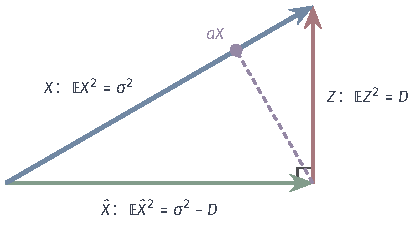
\includegraphics[width=72mm]{figures/07-probability/05-source-coding/tikz/rd-gaussian-geometry/figure.pdf}
  \caption{高斯最优测试信道的均方几何，$\sigma^{2}=1$，$D=\tfrac14$。向量长度表示均方根：绿色$\hat{X}$与红色误差$Z$独立因而正交，合成蓝色的$X$。紫点是$\hat{X}$在$X$方向上的投影$aX$，$a=1-D/\sigma^{2}=\tfrac34$，紫色虚线垂直于$X$。}
  \label{fig:rd-gaussian-geometry}
\end{BookInlineFigure}

\paragraph{各个区间的码率}
式~\eqref{eq:rd-gaussian}的三段各有含义。
\begin{itemize}
  \item $0<D<\sigma^{2}$时，反解得失真率函数$D(R)=\sigma^{2}2^{-2R}$：每多$1$\,bit，均方误差降为四分之一。$\sigma^{2}=1$、$D=\tfrac14$时恰需$1$\,bit。
  \item $D\geq\sigma^{2}$时不需要描述，输出均值即可，零码率失真就是方差。
  \item $D\downarrow0$时$R(D)\to\infty$：连续取值的信源不能用有限码率精确描述，这与有限字母表上$R(0)=H(X)$的情形不同。
\end{itemize}
均值$\mu$只影响平移，不改变码率。退化的$\sigma^{2}=0$是确定的源$X=\mu$，对一切$D\geq0$有$R(D)=0$，公式~\eqref{eq:rd-gaussian}不适用。

\paragraph{编码定理与有限量化器}
定理~\ref{thm:rd-gaussian}是关于信息率失真函数的结论。要说$R(D)$也是高斯信源在平方失真下的最低渐近码率，还需要把编码定理推广到连续字母表与无界失真：可以先把源与重构离散化、截断尾部，在有限字母表上用第~\ref{sec:rd-coding-theorem}节的定理，再控制离散化与尾部带来的误差。结论成立，但证明较长，读者可查阅~\scite{math-cover2006information}。

承认这一点，就能回答开头的第二个问题。图~\ref{fig:rd-gaussian-quantizers}对标准高斯信源比较几类方案。码率为$1$\,bit时，极限是$D(1)=0.25$，而第~\ref{chap:quantization}章的两点最优量化器只做到$1-2/\pi\approx0.363$。反过来看，失真$0.363$只需
\[
  R(0.363)=\frac12\log_2\frac{1}{0.363}\approx0.730
\]
bit，逐个量化多用了约$0.27$\,bit。四点、八点、十六点的Lloyd–Max量化器与极限之间也一直有差距。

\begin{BookInlineFigure}
  \centering
  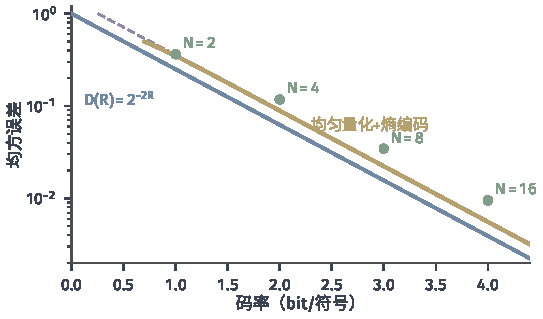
\includegraphics[width=92mm]{figures/07-probability/05-source-coding/matplotlib/rd-gaussian-quantizers/figure.pdf}
  \caption{标准高斯信源在平方失真下的码率与均方误差，纵轴为对数刻度。蓝线是$D(R)=2^{-2R}$。绿点是$N=2,4,8,16$个重构值的Lloyd–Max量化器，码率取定长索引的$\log_2N$。黄线是步长从$3$减小到$0.1$的均匀量化器（重构取区间条件均值），码率取索引的熵，即理想无损压缩索引后的平均长度。紫色虚线是蓝线向右平移$\tfrac12\log_2\frac{\pi\mathrm{e}}{6}\approx0.2546$\,bit。}
  \label{fig:rd-gaussian-quantizers}
\end{BookInlineFigure}

把均匀量化器的索引再作无损压缩（第~\ref{chap:quantization}章），黄线比定长索引好得多，但在高码率时与极限保持一个固定的水平距离。这个距离可以用高分辨率近似估计。步长$\Delta$很小时，均方误差约为$\Delta^{2}/12$，索引的熵约为$h(X)-\log_2\Delta$，所以码率约为
\[
  h(X)-\frac12\log_2(12D).
\]
而由式~\eqref{eq:rd-gaussian}与$h(X)=\frac12\log_2(2\pi\mathrm{e}\sigma^{2})$，$R(D)=h(X)-\frac12\log_2(2\pi\mathrm{e}D)$。两者相减，差距约为
\[
  \frac12\log_2\frac{2\pi\mathrm{e}}{12}=\frac12\log_2\frac{\pi\mathrm{e}}{6}\approx0.2546
\]
bit。这只是近似推导，数值计算印证了它：步长$0.25$时，索引熵为$4.051$\,bit，均方误差为$0.00518$，而这个失真下的$R(D)$约为$3.796$\,bit，差$0.2546$\,bit。逐值量化的格子是一维区间，要再缩小这段差距，只能把许多值合在一起量化，这正是长块编码所做的事。

\subsection{多分量的码率分配}
\label{sec:rd-allocation}

一个测量向量有几个独立的高斯分量，方差各不相同，总的平方误差预算为$D$。码率该怎样分给各分量？直觉是方差大的分量多给，但给多少、方差小的分量是否要给，需要计算。

\paragraph{独立分量的分解}
设$\bm{X}=(X_1,\dots,X_m)$的分量相互独立，$X_k\sim\mathcal{N}(0,\sigma_k^{2})$，$\sigma_k^{2}>0$。把整个向量看成一个源符号，失真取$\lVert\bm{x}-\hat{\bm{x}}\rVert_2^{2}$，$R(D)$表示每个向量所需的bit数。记$R_k(D_k)$为第$k$个分量按式~\eqref{eq:rd-gaussian}的率失真函数，其中$\sigma^{2}$换成$\sigma_k^{2}$。

\begin{theorem}[反注水]
\label{thm:rd-reverse-waterfilling}
在上述设定下，对$0<D<\sum_k\sigma_k^{2}$，
\begin{equation}
  R(D)=\sum_{k=1}^{m}\frac12\log_2\frac{\sigma_k^{2}}{D_k},\qquad D_k=\min\{\theta,\sigma_k^{2}\},
  \label{eq:rd-reverse-waterfilling}
\end{equation}
其中$\theta>0$由$\sum_k\min\{\theta,\sigma_k^{2}\}=D$唯一确定；$D\geq\sum_k\sigma_k^{2}$时$R(D)=0$。
\end{theorem}

\begin{proof}
\emph{下界。}任取满足失真约束的联合分布，设互信息有限。由第~\ref{chap:information-measures}章互信息的链式法则，
\[
  I(\bm{X};\hat{\bm{X}})=\sum_{k=1}^{m}I(X_k;\hat{\bm{X}}\mid X_1,\dots,X_{k-1}).
\]
记$\bm{X}_{<k}=(X_1,\dots,X_{k-1})$，再用链式法则，
\[
  I(X_k;\hat{\bm{X}},\bm{X}_{<k})=I(X_k;\bm{X}_{<k})+I(X_k;\hat{\bm{X}}\mid\bm{X}_{<k}).
\]
分量独立使右端第一项为零，所以第$k$项等于$I(X_k;\hat{\bm{X}},\bm{X}_{<k})$，它不小于$I(X_k;\hat{X}_k)$（数据处理：丢掉一部分观测不增加信息）。

记$D_k=\mathbb{E}(X_k-\hat{X}_k)^{2}$，则$\sum_kD_k\leq D$，并由定理~\ref{thm:rd-gaussian}，$I(X_k;\hat{X}_k)\geq R_k(D_k)$。于是
\[
  I(\bm{X};\hat{\bm{X}})\geq\min\Bigl\{\sum_kR_k(D_k):\ D_k\geq0,\ \sum_kD_k\leq D\Bigr\}.
\]

\emph{达到。}对任意分配$(D_k)$，各分量独立地使用定理~\ref{thm:rd-gaussian}中的最优测试信道（$D_k\geq\sigma_k^{2}$时输出$0$）。各对$(X_k,\hat{X}_k)$相互独立，互信息可加，等于$\sum_kR_k(D_k)$，失真之和为$\sum_kD_k$。所以$R(D)$等于上面这个分配问题的最小值。

\emph{求解分配。}$D_k>\sigma_k^{2}$只浪费预算，可设$0<D_k\leq\sigma_k^{2}$，目标是$\sum_k\frac12\log_2(\sigma_k^{2}/D_k)$，凸且可微，约束是线性的。由KKT条件（可参考\BookChapterRef{chap:constrained-optimality}{卷五第17章“约束问题的最优性”}），存在$\nu\geq0$与$\eta_k\geq0$使
\[
  -\frac{\log_2\mathrm{e}}{2D_k}+\nu+\eta_k=0,\qquad \eta_k\,(D_k-\sigma_k^{2})=0 .
\]
若$D_k<\sigma_k^{2}$，则$\eta_k=0$，于是$\nu>0$，记
\[
  D_k=\frac{\log_2\mathrm{e}}{2\nu}=\theta .
\]
若$D_k=\sigma_k^{2}$，则
\[
  \frac{\log_2\mathrm{e}}{2\sigma_k^{2}}=\nu+\eta_k\geq\nu,
\]
即$\sigma_k^{2}\leq\theta$。两种情形合起来就是$D_k=\min\{\theta,\sigma_k^{2}\}$。凸问题中KKT条件也是充分的，所以这确实是最小点。$\theta\mapsto\sum_k\min\{\theta,\sigma_k^{2}\}$连续、严格递增直到$\sum_k\sigma_k^{2}$，所以$\theta$唯一。
\end{proof}

这个分配称为\term{反注水}（reverse water-filling）。把每个分量的方差画成一根柱子，在高度$\theta$处画一条水平线：高于水平线的分量，失真都是$\theta$，码率是$\frac12\log_2(\sigma_k^{2}/\theta)$；低于水平线的分量干脆不描述，输出$0$，失真就是它的全部方差。方差小的分量本身离$0$不远，花码率描述它不如把预算让给方差大的分量。

\paragraph{一个三分量的例子}
取$\sigma^{2}=(4,1,0.25)$，总失真$D=1.5$。试$\theta\in[0.25,1)$：第三个分量不描述，前两个失真都是$\theta$，
\[
  2\theta+0.25=1.5,\qquad \theta=0.625 ,
\]
确实落在所设区间内。各分量的码率为
\[
  R_1=\frac12\log_2\frac{4}{0.625}\approx1.339,\qquad
  R_2=\frac12\log_2\frac{1}{0.625}\approx0.339,\qquad R_3=0 .
\]
合计约$1.678$\,bit每向量，平均每个分量约$0.559$\,bit，平均每个分量的失真是$1.5/3=0.5$。总量与每分量平均量之间只差一个因子$m$，比较时两者不能混用。

作为对照，把预算平分，每个分量都给$0.5$。第三个分量的方差只有$0.25$，给它$0.5$的失真预算用不完，它实际只产生$0.25$的失真；前两个分量需要
\[
  \frac12\log_2\frac{4}{0.5}+\frac12\log_2\frac{1}{0.5}=1.5+0.5=2
\]
bit，比反注水多出约$0.32$\,bit，总失真却只有$1.25$，浪费了预算。

图~\ref{fig:rd-reverse-waterfilling}(a)画出这个分配，(b)画出总码率随总失真的变化。$D=0.75$时水平线降到$0.25$，第三个分量开始需要描述；$D=2.25$时水平线升到$1$，第二个分量不再描述。在这两个折点，曲线的组成方式改变，但仍连续且凸。

\begin{BookInlineFigure}
  \centering
  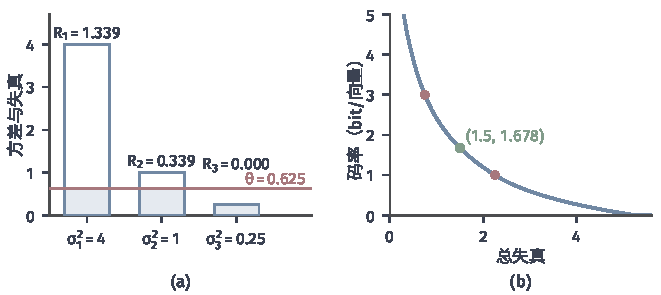
\includegraphics[width=112mm]{figures/07-probability/05-source-coding/matplotlib/rd-reverse-waterfilling/figure.pdf}
  \caption{方差为$(4,1,0.25)$的独立高斯分量的反注水。(a)总失真$1.5$时的分配：蓝框是各分量方差，浅蓝填充是分到的失真$D_k=\min\{\theta,\sigma_k^{2}\}$，红线是水平$\theta=0.625$，柱上方是各分量的码率（bit）。(b)每向量的总码率随总失真的变化；红点是分量开始或停止被描述的折点$D=0.75$与$D=2.25$，绿点是(a)中的分配。}
  \label{fig:rd-reverse-waterfilling}
\end{BookInlineFigure}

\paragraph{相关的高斯向量}
分量相关时先旋转坐标。设$\bm{X}\sim\mathcal{N}(\bm{0},\bm{\Sigma})$，协方差矩阵$\bm{\Sigma}$有正交特征分解$\bm{\Sigma}=\bm{U}\bm{\Lambda}\bm{U}^{\top}$，$\bm{\Lambda}$为特征值$\lambda_1,\dots,\lambda_m$组成的对角矩阵。令$\bm{Y}=\bm{U}^{\top}\bm{X}$，则$\bm{Y}\sim\mathcal{N}(\bm{0},\bm{\Lambda})$，各分量不相关。由第~\ref{chap:multivariate-distributions}章，联合高斯向量的分量不相关即独立。

旋转不改变问题。对任意重构$\hat{\bm{X}}$，令$\hat{\bm{Y}}=\bm{U}^{\top}\hat{\bm{X}}$。正交矩阵保持长度，
\[
  \lVert\bm{X}-\hat{\bm{X}}\rVert_2^{2}=\lVert\bm{Y}-\hat{\bm{Y}}\rVert_2^{2};
\]
$\bm{U}^{\top}$是可逆的连续映射，由第~\ref{chap:information-measures}章，双方向可测的一一变换保持互信息，$I(\bm{X};\hat{\bm{X}})=I(\bm{Y};\hat{\bm{Y}})$。所以两个问题的可行集合一一对应，目标值相同，$\bm{X}$的$R(D)$就是对特征值$\lambda_k$作反注水。

例如$\bm{\Sigma}=\begin{bmatrix}2&1\\1&2\end{bmatrix}$，特征值为$3$与$1$，特征向量为$(1,1)/\sqrt2$与$(-1,1)/\sqrt2$。总失真$D=1$时，试$\theta<1$，得$2\theta=1$，$\theta=0.5$，
\[
  R(1)=\frac12\log_2\frac{3}{0.5}+\frac12\log_2\frac{1}{0.5}\approx1.292+0.5=1.792
\]
bit每向量。若忽略相关性，把$X_1,X_2$当作两个方差为$2$的信源分别描述，最好的分法是各给$0.5$，需要$\frac12\log_2\frac{2}{0.5}\times2=2$\,bit。联合描述省下约$0.21$\,bit，来源于旋转后两个方向的方差不再相等，反注水可以把预算向方差大的方向倾斜。

\begin{BookInlineFigure}
  \centering
  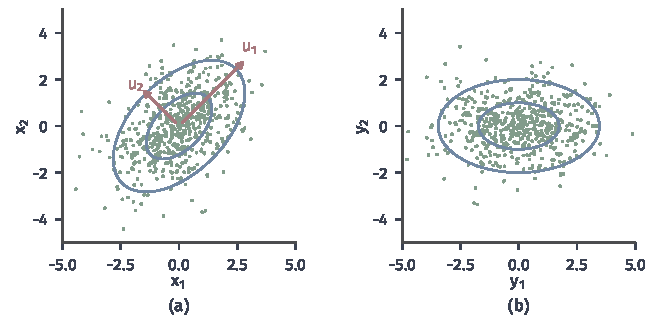
\includegraphics[width=112mm]{figures/07-probability/05-source-coding/matplotlib/rd-correlated-rotation/figure.pdf}
  \caption{相关高斯向量的旋转，$\bm{\Sigma}=\begin{bmatrix}2&1\\1&2\end{bmatrix}$，$600$个样本（绿），随机种子$722$。(a)原坐标中的样本与一倍、两倍标准差的等密度椭圆（蓝），红箭头是特征方向$\bm{u}_1,\bm{u}_2$。(b)旋转后$\bm{Y}=\bm{U}^{\top}\bm{X}$的样本，两个坐标不相关，方差分别为$3$与$1$。}
  \label{fig:rd-correlated-rotation}
\end{BookInlineFigure}

图~\ref{fig:rd-correlated-rotation}显示了旋转的作用：原坐标中两个分量一起变化，旋转后椭圆的轴与坐标轴对齐。旋转本身不改变失真和信息，它只是把问题变成可以逐分量求解的形式；码率的分配仍由特征值与水平$\theta$决定。


\section{率失真函数的计算}
\label{sec:rd-computation}

一般的有限概率表没有闭式解。第~\ref{sec:rd-feasible-range}节的三元例子只在$D_{\min}$一点能手算，整条曲线就需要数值方法。式~\eqref{eq:rd-information-rd}是一个凸优化问题，但目标中的$r_q$又依赖$q$，直接求解并不方便。Blahut–Arimoto算法把它拆成两个都有闭式解的子问题，交替求解。本节设$\mathcal{X},\hat{\mathcal{X}}$有限，$p(x)>0$对一切$x$成立（概率为零的源值可以删去），失真矩阵$d(x,\hat{x})$取非负有限值。

\paragraph{用乘子去掉约束}
失真约束先换成罚项。对$s\geq0$，令
\begin{equation}
  F_s^{\star}=\min_{q}\Bigl[I(P_X,q)+s\,\mathbb{E}d(X,\hat{X})\Bigr],
  \label{eq:rd-lagrangian}
\end{equation}
$s$称为失真乘子，单位是bit每单位失真。最小值存在，因为目标在测试信道的紧集上连续。

设$q_s$是一个最小点，$D_s$是它的平均失真。若有平均失真不超过$D_s$而互信息更小的测试信道，它的目标值也更小，与$q_s$最小矛盾。所以$I(P_X,q_s)=R(D_s)$，最小点总落在率失真曲线上。

在码率—失真平面上，目标值为常数$F$的点组成斜率为$-s$的直线$R=F-sD$。求最小就是把这条直线从下方向上平移，直到碰到可行点，第一次碰到的位置就是曲线上斜率为$-s$的切点。图~\ref{fig:rd-ba-curves}(b)画出了三条这样的支撑直线。改变$s$，切点沿曲线移动：$s$大表示失真贵，切点靠近$D_{\min}$；$s$小表示码率贵，切点靠近$D_{\max}$。

\paragraph{两个变量的目标}
困难在于$I(P_X,q)$的分母$r_q$也随$q$变化。把它换成一个自由变量。对$\hat{\mathcal{X}}$上的任一分布$r$（在$r_q>0$处$r>0$），按$\hat{x}$合并后可得
\[
  \sum_{x,\hat{x}}p(x)q(\hat{x}\mid x)\log_2\frac{q(\hat{x}\mid x)}{r(\hat{x})}
  =I(P_X,q)+\sum_{\hat{x}}r_q(\hat{x})\log_2\frac{r_q(\hat{x})}{r(\hat{x})},
\]
最后一项是$D_{\mathrm{KL}}(r_q\Vert r)\geq0$，$r=r_q$时为零。所以互信息是左端对$r$的最小值。

于是令
\begin{equation}
  J(q,r)=\sum_{x}p(x)\sum_{\hat{x}}q(\hat{x}\mid x)\Bigl[\log_2\frac{q(\hat{x}\mid x)}{r(\hat{x})}+s\,d(x,\hat{x})\Bigr],
  \label{eq:rd-ba-objective}
\end{equation}
则$F_s^{\star}=\min_{q,r}J(q,r)$。对两个变量交替求最小，每一步都有闭式解。

\paragraph{固定$r$求$q$}
引入
\begin{equation}
  Z_r(x)=\sum_{\hat{x}}r(\hat{x})\,2^{-s\,d(x,\hat{x})},\qquad
  w_r(\hat{x}\mid x)=\frac{r(\hat{x})\,2^{-s\,d(x,\hat{x})}}{Z_r(x)}.
  \label{eq:rd-ba-q-update}
\end{equation}
$w_r(\cdot\mid x)$是一个概率分布：把当前的重构边缘乘以失真的指数权重$2^{-sd}$，再归一化。由$s\,d=-\log_2(2^{-sd})$，式~\eqref{eq:rd-ba-objective}方括号中的量可以写成
\[
  \log_2\frac{q(\hat{x}\mid x)}{r(\hat{x})2^{-s\,d(x,\hat{x})}}=\log_2\frac{q(\hat{x}\mid x)}{w_r(\hat{x}\mid x)}-\log_2Z_r(x).
\]
代回去，得到
\[
  J(q,r)=\sum_{x}p(x)\,D_{\mathrm{KL}}\bigl(q(\cdot\mid x)\Vert w_r(\cdot\mid x)\bigr)-\sum_{x}p(x)\log_2Z_r(x).
\]
KL散度非负且只在两分布相同时为零，所以固定$r$时最优的$q$恰是$w_r$，最小值为
\begin{equation}
  J(w_r,r)=-\sum_{x}p(x)\log_2Z_r(x).
  \label{eq:rd-ba-j-value}
\end{equation}

式~\eqref{eq:rd-ba-q-update}有直观的含义：给定$x$，一个重构值被选中的机会正比于两件事的乘积，一是它在当前方案中被用到的频率$r(\hat{x})$，二是它离$x$有多近。失真每增加$1$，权重就乘以$2^{-s}$。

\paragraph{固定$q$求$r$}
由前面的分解，固定$q$时最优的$r$就是$r_q$，即式~\eqref{eq:rd-output-marginal}。把两步合起来，新的重构边缘是
\begin{equation}
  r^{\mathrm{new}}(\hat{x})=\sum_{x}p(x)\,w_r(\hat{x}\mid x)=r(\hat{x})\,c_r(\hat{x}),\qquad
  c_r(\hat{x})=\sum_{x}\frac{p(x)\,2^{-s\,d(x,\hat{x})}}{Z_r(x)} .
  \label{eq:rd-ba-r-update}
\end{equation}
$c_r(\hat{x})$是一个乘性修正因子：大于$1$的重构值在新方案中被用得更多。由$Z_r$的定义，
\[
  \sum_{\hat{x}}r(\hat{x})c_r(\hat{x})=\sum_{x}\frac{p(x)}{Z_r(x)}\sum_{\hat{x}}r(\hat{x})2^{-s\,d(x,\hat{x})}=\sum_xp(x)=1,
\]
所以$r^{\mathrm{new}}$仍是概率分布，且$\max_{\hat{x}}c_r(\hat{x})\geq1$。若某个$r(\hat{x})=0$，它以后永远为零，因此初值必须处处为正。

\paragraph{计算过程}
下面结合同一个例子写出计算过程。仍取$X\sim\operatorname{Bern}(0.3)$与Hamming失真，乘子取$s=\log_29\approx3.170$，于是一次错误的权重是$2^{-s}=\tfrac19$。由第~\ref{sec:rd-binary}节，$R'(D)=-\log_2\frac{1-D}{D}$，斜率为$-\log_29$的点是$D=0.1$，所以算法应收敛到$R(0.1)\approx0.4123$，目标最优值为
\[
  F_s^{\star}=R(0.1)+0.1\log_29\approx0.4123+0.3170=0.7293 .
\]

\needspace{6\baselineskip}
\paragraph{变量}
\begin{itemize}
  \item $\bm{A}$：$\lvert\mathcal{X}\rvert\times\lvert\hat{\mathcal{X}}\rvert$矩阵，元素$a_{x,\hat{x}}=2^{-s\,d(x,\hat{x})}$，计算一次后不变。例中$\bm{A}=\begin{bmatrix}1&1/9\\1/9&1\end{bmatrix}$。
  \item $r$：长度$\lvert\hat{\mathcal{X}}\rvert$的概率向量，当前重构边缘$r^{(t)}$。
  \item $Z$：长度$\lvert\mathcal{X}\rvert$的向量，归一化常数$Z^{(t)}(x)$。
  \item $q$：$\lvert\mathcal{X}\rvert\times\lvert\hat{\mathcal{X}}\rvert$矩阵，本轮的测试信道$q^{(t+1)}$，每行和为$1$。
  \item $c$：长度$\lvert\hat{\mathcal{X}}\rvert$的修正因子。
  \item $J^{(t+1)}$与$\epsilon^{(t+1)}$：本轮目标值与最优性误差界，用于停止判断；$D^{(t+1)}$与$I^{(t+1)}$：本轮测试信道的平均失真与互信息，用于报告结果。
\end{itemize}

\paragraph{初始化}
$r^{(0)}$取处处为正的分布，常用均匀分布；给定停止容差$\varepsilon>0$与最大轮数。例中
\[
  r^{(0)}=(0.5,\,0.5),\qquad \varepsilon=10^{-3}.
\]

\needspace{6\baselineskip}
\paragraph{每轮更新}
第$t+1$轮（$t=0,1,\dots$）：
\begin{enumerate}
  \item \textbf{归一化常数。}按式~\eqref{eq:rd-ba-q-update}，取$r=r^{(t)}$算出$Z^{(t)}(x)$，即矩阵$\bm{A}$的第$x$行与$r^{(t)}$的内积。例中第一轮
  \[
    Z^{(0)}(0)=0.5+\frac{0.5}{9}=\frac59,\qquad Z^{(0)}(1)=\frac{0.5}{9}+0.5=\frac59 .
  \]

  \item \textbf{测试信道。}按式~\eqref{eq:rd-ba-q-update}，$q^{(t+1)}$的第$x$行是$r^{(t)}$与$\bm{A}$第$x$行的逐元素乘积除以$Z^{(t)}(x)$。例中第一轮
  \[
    \begin{gathered}
    q^{(1)}(0\mid0)=\frac{0.5}{5/9}=0.9,\qquad q^{(1)}(1\mid0)=0.1,\\
    q^{(1)}(1\mid1)=0.9,\qquad q^{(1)}(0\mid1)=0.1 ,
    \end{gathered}
  \]
  正是第~\ref{sec:rd-test-channels}节以$0.1$翻转的测试信道。

  \item \textbf{目标值。}由式~\eqref{eq:rd-ba-j-value}，$J^{(t+1)}=-\sum_xp(x)\log_2Z^{(t)}(x)$。例中第一轮
  \[
    J^{(1)}=-\log_2\frac59\approx0.8480 .
  \]

  \item \textbf{修正因子与新边缘。}按式~\eqref{eq:rd-ba-r-update}算$c$与$r^{(t+1)}=r^{(t)}c$。例中第一轮
  \[
    c(0)=\frac{0.7\times1+0.3\times\frac19}{5/9}=1.32,\qquad c(1)=\frac{0.7\times\frac19+0.3\times1}{5/9}=0.68,
  \]
  \[
    r^{(1)}=(0.5\times1.32,\ 0.5\times0.68)=(0.66,\ 0.34).
  \]

  \item \textbf{误差界与停止。}令$\epsilon^{(t+1)}=\max_{\hat{x}}\log_2c(\hat{x})$。下面的定理~\ref{thm:rd-ba-bounds}说明最优值被夹在$J^{(t+1)}-\epsilon^{(t+1)}$与$J^{(t+1)}$之间。若$\epsilon^{(t+1)}\leq\varepsilon$则停止，否则进入下一轮。例中第一轮
  \[
    \epsilon^{(1)}=\log_21.32\approx0.4005,
  \]
  所以$F_s^{\star}\in[0.4475,\,0.8480]$，继续。

  \item \textbf{报告量。}按式~\eqref{eq:rd-test-distortion}与式~\eqref{eq:rd-test-information}算$q^{(t+1)}$的平均失真$D^{(t+1)}$与互信息$I^{(t+1)}$。例中第一轮
  \[
    D^{(1)}=0.1,\qquad I^{(1)}\approx0.4558 .
  \]
\end{enumerate}

第二轮从$r^{(1)}=(0.66,0.34)$出发：
\[
  Z^{(1)}(0)=0.66+\frac{0.34}{9}\approx0.6978,\qquad Z^{(1)}(1)=\frac{0.66}{9}+0.34\approx0.4133 .
\]
测试信道变为$q^{(2)}(1\mid0)\approx0.0541$，$q^{(2)}(0\mid1)\approx0.1774$，错误开始向罕见符号转移。目标值与修正因子为
\[
  J^{(2)}\approx0.7458,\qquad c\approx(1.0838,\ 0.8373),\qquad r^{(2)}\approx(0.7153,\ 0.2847),
\]
误差界$\epsilon^{(2)}\approx0.1161$，报告量$D^{(2)}\approx0.0911$，$I^{(2)}\approx0.4468$。

此后各轮的结果列在表~\ref{tab:rd-ba-rounds}中。误差界每轮约缩小为原来的$0.4$倍，第$7$轮的误差界约为$1.2\times10^{-3}$，第$8$轮约为$5.1\times10^{-4}$，首次低于$\varepsilon$，停止。最终得到
\[
  \begin{gathered}
  q^{(8)}(1\mid0)\approx0.0358,\qquad q^{(8)}(0\mid1)\approx0.2495,\\
  D^{(8)}\approx0.0999,\qquad I^{(8)}\approx0.4125 ,
  \end{gathered}
\]
与精确解$q(1\mid0)=\tfrac1{28}\approx0.0357$、$q(0\mid1)=0.25$、$(D,R)=(0.1,0.4123)$相差不到$10^{-3}$。

\begin{BookInlineTable}
  \centering
  \caption{Blahut–Arimoto算法在例中的各轮结果，$s=\log_29$，$r^{(0)}=(0.5,0.5)$。$r^{(t)}(1)$是本轮更新后的重构边缘，其余各量由本轮开始时的边缘$r^{(t-1)}$算出。}
  \label{tab:rd-ba-rounds}
  \begin{tabular}{cccccc}
    \toprule
    $t$ & $r^{(t)}(1)$ & $J^{(t)}$ & $\epsilon^{(t)}$ & $D^{(t)}$ & $I^{(t)}$ \\
    \midrule
    $1$ & $0.3400$ & $0.8480$ & $0.4005$ & $0.1000$ & $0.4558$ \\
    $2$ & $0.2847$ & $0.7458$ & $0.1161$ & $0.0911$ & $0.4468$ \\
    $3$ & $0.2642$ & $0.7318$ & $0.0408$ & $0.0951$ & $0.4288$ \\
    $4$ & $0.2559$ & $0.7297$ & $0.0160$ & $0.0978$ & $0.4196$ \\
    $5$ & $0.2525$ & $0.7294$ & $0.0066$ & $0.0990$ & $0.4155$ \\
    $6$ & $0.2511$ & $0.7293$ & $0.0028$ & $0.0996$ & $0.4137$ \\
    $7$ & $0.2505$ & $0.7293$ & $0.0012$ & $0.0998$ & $0.4129$ \\
    $8$ & $0.2502$ & $0.7293$ & $0.0005$ & $0.0999$ & $0.4125$ \\
    \bottomrule
  \end{tabular}
\end{BookInlineTable}

\paragraph{误差界}
停止条件依赖一个可计算的最优性误差界。它来自对任意测试信道成立的一个下界。

\begin{theorem}[Blahut–Arimoto的上下界]
\label{thm:rd-ba-bounds}
对任一处处为正的分布$r$，记$Z_r,w_r,c_r$如式~\eqref{eq:rd-ba-q-update}与式~\eqref{eq:rd-ba-r-update}。则对任意测试信道$q$，
\begin{equation}
  I(P_X,q)+s\,\mathbb{E}_qd\geq-\sum_{x}p(x)\log_2Z_r(x)-\sum_{\hat{x}}r_q(\hat{x})\log_2c_r(\hat{x}),
  \label{eq:rd-ba-lower}
\end{equation}
因而
\begin{equation}
  -\sum_xp(x)\log_2Z_r(x)-\max_{\hat{x}}\log_2c_r(\hat{x})\leq F_s^{\star}\leq-\sum_xp(x)\log_2Z_r(x).
  \label{eq:rd-ba-bounds}
\end{equation}
\end{theorem}

\begin{proof}
由$J$的分解，取$r=r_q$时$J(q,r_q)=I(P_X,q)+s\,\mathbb{E}_qd$。下面用$w_r$改写$J(q,r_q)$。由$w_r$的定义，$2^{s\,d}=r/(w_rZ_r)$，于是
\[
  \log_2\frac{q(\hat{x}\mid x)\,2^{s\,d(x,\hat{x})}}{r_q(\hat{x})}
  =\log_2\frac{q(\hat{x}\mid x)}{w_r(\hat{x}\mid x)}+\log_2\frac{r(\hat{x})}{r_q(\hat{x})}-\log_2Z_r(x).
\]
按$p(x)q(\hat{x}\mid x)$求和，左端是$I(P_X,q)+s\,\mathbb{E}_qd$，右端第三项给出$-\sum_xp(x)\log_2Z_r(x)$，第二项给出$-D_{\mathrm{KL}}(r_q\Vert r)$。

第一项对每个$\hat{x}$用引理~\ref{lem:rd-log-sum}，以$a_x=p(x)q(\hat{x}\mid x)$、$b_x=p(x)w_r(\hat{x}\mid x)$合并$x$：
\[
  \sum_{x,\hat{x}}p(x)q(\hat{x}\mid x)\log_2\frac{q(\hat{x}\mid x)}{w_r(\hat{x}\mid x)}
  \geq\sum_{\hat{x}}r_q(\hat{x})\log_2\frac{r_q(\hat{x})}{r(\hat{x})c_r(\hat{x})},
\]
这里用了式~\eqref{eq:rd-ba-r-update}：$w_r$的输出边缘是$rc_r$。右端等于$D_{\mathrm{KL}}(r_q\Vert r)-\sum_{\hat{x}}r_q(\hat{x})\log_2c_r(\hat{x})$。

三项相加，$D_{\mathrm{KL}}(r_q\Vert r)$恰好抵消，得到式~\eqref{eq:rd-ba-lower}。右端最后一项不超过$\max_{\hat{x}}\log_2c_r(\hat{x})$，对$q$取最小即得式~\eqref{eq:rd-ba-bounds}的左半。右半来自$w_r$本身的目标值：它不小于$F_s^{\star}$，又不超过$J(w_r,r)$，而后者由式~\eqref{eq:rd-ba-j-value}给出。
\end{proof}

误差界$\max_{\hat{x}}\log_2c_r(\hat{x})$为零，当且仅当所有$c_r(\hat{x})\leq1$；由$\sum_{\hat{x}}rc_r=1$，这时在$r>0$处$c_r=1$，$r$是更新的不动点。所以$\epsilon$同时度量“离不动点多远”与“离最优值多远”。

\paragraph{收敛}
误差界说明了何时可以停止，但没有说明它一定会变小。下面的定理给出目标值的收敛速度。

\begin{theorem}[目标值的收敛]
\label{thm:rd-ba-convergence}
设初值$r^{(0)}$处处为正，按上面的两步交替迭代，$J^{(t)}$是由$r^{(t-1)}$按式~\eqref{eq:rd-ba-j-value}算出的目标值。设$q^{\star}$是式~\eqref{eq:rd-lagrangian}的一个最小点，$r^{\star}=r_{q^{\star}}$。则$J^{(t)}$非增，并且
\begin{equation}
  J^{(T)}-F_s^{\star}\leq\frac{D_{\mathrm{KL}}(r^{\star}\Vert r^{(0)})}{T},\qquad T=1,2,\dots .
  \label{eq:rd-ba-rate}
\end{equation}
\end{theorem}

\begin{proof}
\emph{单调。}$J^{(t+1)}$是$J(\cdot,r^{(t)})$的最小值，$r^{(t)}$又是$J(q^{(t)},\cdot)$的最小点，所以
\[
  J^{(t+1)}=\min_qJ(q,r^{(t)})\leq J(q^{(t)},r^{(t)})\leq J(q^{(t)},r^{(t-1)})=J^{(t)}.
\]

\emph{每轮的进展。}在式~\eqref{eq:rd-ba-lower}中取$q=q^{\star}$与$r=r^{(t)}$，左端是$F_s^{\star}$，于是
\[
  J^{(t+1)}-F_s^{\star}\leq\sum_{\hat{x}}r^{\star}(\hat{x})\log_2c_{r^{(t)}}(\hat{x}).
\]
由式~\eqref{eq:rd-ba-r-update}，$c_{r^{(t)}}=r^{(t+1)}/r^{(t)}$。初值处处为正，而$2^{-sd}>0$使每个$c$为正，所以各$r^{(t)}$处处为正，右端可以写成
\[
  \sum_{\hat{x}}r^{\star}(\hat{x})\log_2\frac{r^{(t+1)}(\hat{x})}{r^{(t)}(\hat{x})}
  =D_{\mathrm{KL}}(r^{\star}\Vert r^{(t)})-D_{\mathrm{KL}}(r^{\star}\Vert r^{(t+1)}).
\]

\emph{求和。}对$t=0,\dots,T-1$相加，右端逐项相消，
\[
  \sum_{t=1}^{T}\bigl(J^{(t)}-F_s^{\star}\bigr)\leq D_{\mathrm{KL}}(r^{\star}\Vert r^{(0)})-D_{\mathrm{KL}}(r^{\star}\Vert r^{(T)})\leq D_{\mathrm{KL}}(r^{\star}\Vert r^{(0)}).
\]
由单调性，左端每一项都不小于$J^{(T)}-F_s^{\star}$，于是得到式~\eqref{eq:rd-ba-rate}。
\end{proof}

初值处处为正保证$D_{\mathrm{KL}}(r^{\star}\Vert r^{(0)})$有限；若某个最优重构值的初始概率为零，它永远回不来，算法可能停在非最优点。由$F_s^{\star}\leq I^{(t)}+sD^{(t)}\leq J^{(t)}$，所报告测试信道的目标值也以同样的速度逼近最优值；再由测试信道集合的紧性与目标的连续性，$q^{(t)}$的每个极限点都是最小点。

例中$r^{\star}=(0.75,0.25)$，
\[
  D_{\mathrm{KL}}(r^{\star}\Vert r^{(0)})=0.75\log_21.5+0.25\log_20.5\approx0.1887 .
\]
式~\eqref{eq:rd-ba-rate}保证第$8$轮的误差不超过$0.024$，实际误差只有约$4\times10^{-7}$。图~\ref{fig:rd-ba-iterations}显示，这个例子中误差按几何速度下降，比$1/T$快得多；$1/T$是对一切有限概率表都成立的保证，几何速度则依赖具体问题。

\begin{BookInlineFigure}
  \centering
  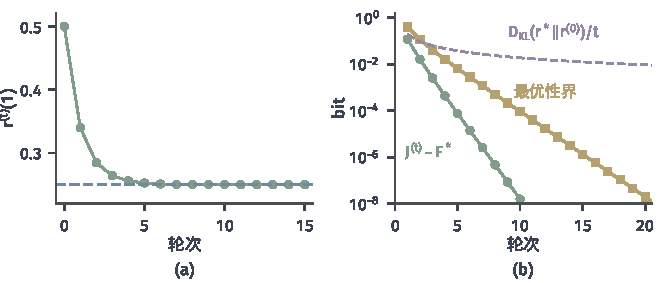
\includegraphics[width=112mm]{figures/07-probability/05-source-coding/matplotlib/rd-ba-iterations/figure.pdf}
  \caption{Blahut–Arimoto算法在例中的收敛，$s=\log_29$，$r^{(0)}=(0.5,0.5)$。(a)重构边缘$r^{(t)}(1)$（绿），蓝色虚线是极限$0.25$。(b)对数刻度下的目标误差$J^{(t)}-F_s^{\star}$（绿）、可计算的误差界$\epsilon^{(t)}=\max\log_2c$（黄）与定理~\ref{thm:rd-ba-convergence}的保证$D_{\mathrm{KL}}(r^{\star}\Vert r^{(0)})/t$（紫色虚线）。}
  \label{fig:rd-ba-iterations}
\end{BookInlineFigure}

\paragraph{改变乘子描出曲线}
每个$s$只给出曲线上的一个点$(D^{(t)},I^{(t)})$，失真不是事先指定的。要得到整条曲线，就对一列$s$分别运行；要求指定$D$处的$R(D)$，就利用$D_s$随$s$增大而不增，对$s$作二分。图~\ref{fig:rd-ba-curves}(a)对$24$个$s$运行算法，所得的点都落在式~\eqref{eq:rd-binary}的曲线上。

\begin{BookInlineFigure}
  \centering
  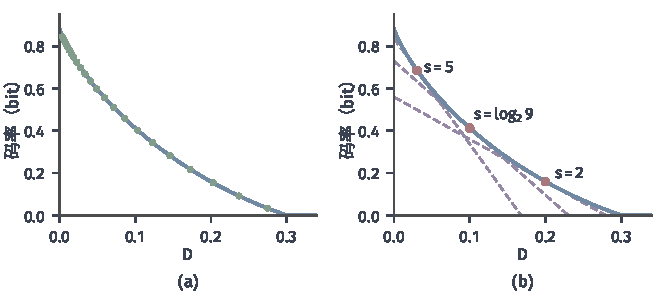
\includegraphics[width=112mm]{figures/07-probability/05-source-coding/matplotlib/rd-ba-curves/figure.pdf}
  \caption{改变乘子描出$\operatorname{Bern}(0.3)$与Hamming失真的率失真曲线。(a)$s$从$1.4$到$8$等距取$24$个值，算法的输出（绿点）落在闭式曲线$h_2(0.3)-h_2(D)$（蓝）上。(b)$s=2,\log_29,5$时目标的等值线$R=F_s^{\star}-sD$（紫色虚线）是曲线的支撑直线，红点是切点$D_s=1/(1+2^{s})$。}
  \label{fig:rd-ba-curves}
\end{BookInlineFigure}

$s$很小时，码率极贵，最优点停在零码率处。例中曲线在$D_{\max}=0.3$左侧的斜率是$-\log_2\frac{0.7}{0.3}\approx-1.222$，所以$s\leq1.222$时最小点是$(0.3,0)$；这时迭代中$r^{(t)}(1)$缓慢趋于零，收敛变慢。$s\to\infty$时切点趋于$D_{\min}$，但对有限的$s$一般到不了端点。$R(D_{\min})$可以另算：只允许把每个$x$送到使$d(x,\cdot)$最小的重构值，在这个子集上最小化互信息，这是同一类型、失真项消失的问题；第~\ref{sec:rd-feasible-range}节的三元例子就是这样算出$0.6$的。

\paragraph{线性区段}
若$R(D)$在某个区间$[D_1,D_2]$上是直线，斜率为$-s_0$，则$s=s_0$时这一段上的所有点都使式~\eqref{eq:rd-lagrangian}最小，算法收敛到哪一个取决于初值，改变$s$也只会在两个端点之间跳跃。这时先用略大和略小于$s_0$的乘子求出两个端点的测试信道，中间的点用它们的混合得到：由引理~\ref{lem:rd-mi-convex}，混合信道的互信息不超过弦的高度，而在线性区段上弦就是曲线本身。在块编码中，这对应于两种码的分时。反过来，曲线在某点有折角时，一段$s$都对应同一个点，二分得到的$D_s$会在这里停留。

\paragraph{计算代价}
每轮要算$Z$、$q$、$c$，各需$O(\lvert\mathcal{X}\rvert\lvert\hat{\mathcal{X}}\rvert)$次运算，存储$\bm{A}$与$q$需要同样大小的空间。数值上，$s$很大时$2^{-sd}$可能下溢，常把每行的指数减去该行的最小失真再计算，归一化后结果不变。还需注意算法求出的是信息率失真函数及其测试信道。它告诉我们极限是多少，以及随机码本应按什么边缘生成，但不给出有限块长的编码器。


\section{本章小结}
\label{sec:rd-summary}

本章回答了开头的两个问题。下雨概率为$0.3$的记录，允许错$10\%$时每天只需$R(0.1)=h_2(0.3)-h_2(0.1)\approx0.412$\,bit，不到无损所需的一半。标准高斯测量值每个$1$\,bit时，长块编码的均方误差极限是$0.25$，逐个量化的最好结果是$0.363$。两处都是“允许失真的最低渐近码率”与“有限方案实际做到的”之间的比较。

这个比较涉及三个层次的对象，它们回答不同的问题，使用的标准必须相同：同一个源分布、同一个失真函数、期望失真、以每个源符号的bit数计的码率。
\begin{itemize}
  \item 有限方案，如第~\ref{chap:quantization}章的量化器或第~\ref{sec:rd-block-model}节的小块长码，可以直接执行，性能可以精确计算，但只是可达区域中的一个点。
  \item 信息率失真函数$R(D)$是单个符号上的凸优化：在平均失真不超过$D$的测试信道中最小化互信息。它非增、凸，在$[D_{\min},D_{\max}]$上严格递减，可以解析或数值地求出。
  \item 操作率失真函数$R_{\mathrm{op}}(D)$是所有块长、所有码本的极限。编码定理说明，对有限字母表、无记忆信源与有界可分失真，它与$R(D)$相等。
\end{itemize}

编码定理的两半依赖不同的工具。下界从“编号只有$M$个值”出发，经数据处理、独立性与链式法则拆成单个符号，再用互信息对测试信道的凸性合并；无记忆性与可分失真在其中缺一不可。可达性用随机码本：按最优测试信道的重构边缘撒点，大数律使信息密度集中在$R(D)$附近，码字数略多于$2^{nR(D)}$就能以高概率覆盖源块，再由平均推出好码本存在。

\begin{BookInlineTable}
  \centering
  \caption{贯穿例子中几类方案的比较。上半部分为$\operatorname{Bern}(0.3)$信源与Hamming失真，下半部分为标准高斯信源与平方失真。}
  \label{tab:rd-summary}
  \begin{tabular}{lcc}
    \toprule
    方案 & 码率（bit/符号） & 平均失真 \\
    \midrule
    逐位照传 & $1$ & $0$ \\
    块长$3$，码本$\{000,100,010,001\}$ & $0.667$ & $0.081$ \\
    块长$4$，最优$4$码字码本 & $0.5$ & $0.136$ \\
    率失真极限$R(D)$ & $0.412$ & $0.1$ \\
    率失真极限$D(R)$ & $0.5$ & $0.074$ \\
    \midrule
    两点Lloyd–Max量化器 & $1$ & $0.363$ \\
    均匀量化加索引熵编码（步长$1$） & $2.105$ & $0.077$ \\
    率失真极限$D(R)=2^{-2R}$ & $1$ & $0.25$ \\
    \bottomrule
  \end{tabular}
\end{BookInlineTable}

解析解都来自同一个两步法：一个对所有测试信道成立的信息下界，加一个达到它的反向测试信道。二元信源的下界来自错误指示的熵，高斯信源的下界来自条件高斯参考与KL非负，后者与固定方差的熵上界是同一个论证。独立高斯分量的码率按反注水分配，方差低于水平的分量不描述；相关分量先按协方差的特征方向旋转，再对特征值反注水。

有限概率表用Blahut–Arimoto算法计算。乘子$s$把失真约束变成罚项，最小点是曲线上斜率为$-s$的切点；交替地用“当前边缘乘以失真的指数权重再归一化”更新测试信道、用输出边缘更新$r$，目标单调下降，误差界$\max\log_2c$可以随时计算，目标误差至少按$1/T$缩小。

求出$R(D)$还没有给出编码器。它给出的是标准：一个有限方案离极限还有多远，例如高分辨率下均匀量化加熵编码约差$0.254$\,bit，这一段只能靠联合处理多个值去缩小；以及若用随机码本，码字应按什么分布生成。有限块长的最优码与低复杂度的搜索不由本章的定理给出。

描述一个信源需要$R(D)$的码率，这些bit还要经过有噪声的信道传出去。下一部分研究信道每次使用能可靠传送多少bit，即信道容量，再把所需的描述资源与可用的传输资源放在一起比较。


